%aQGC results
All log-likelihood distributions are shown.

%FT0
\begin{figure}[ht]
    \centering
    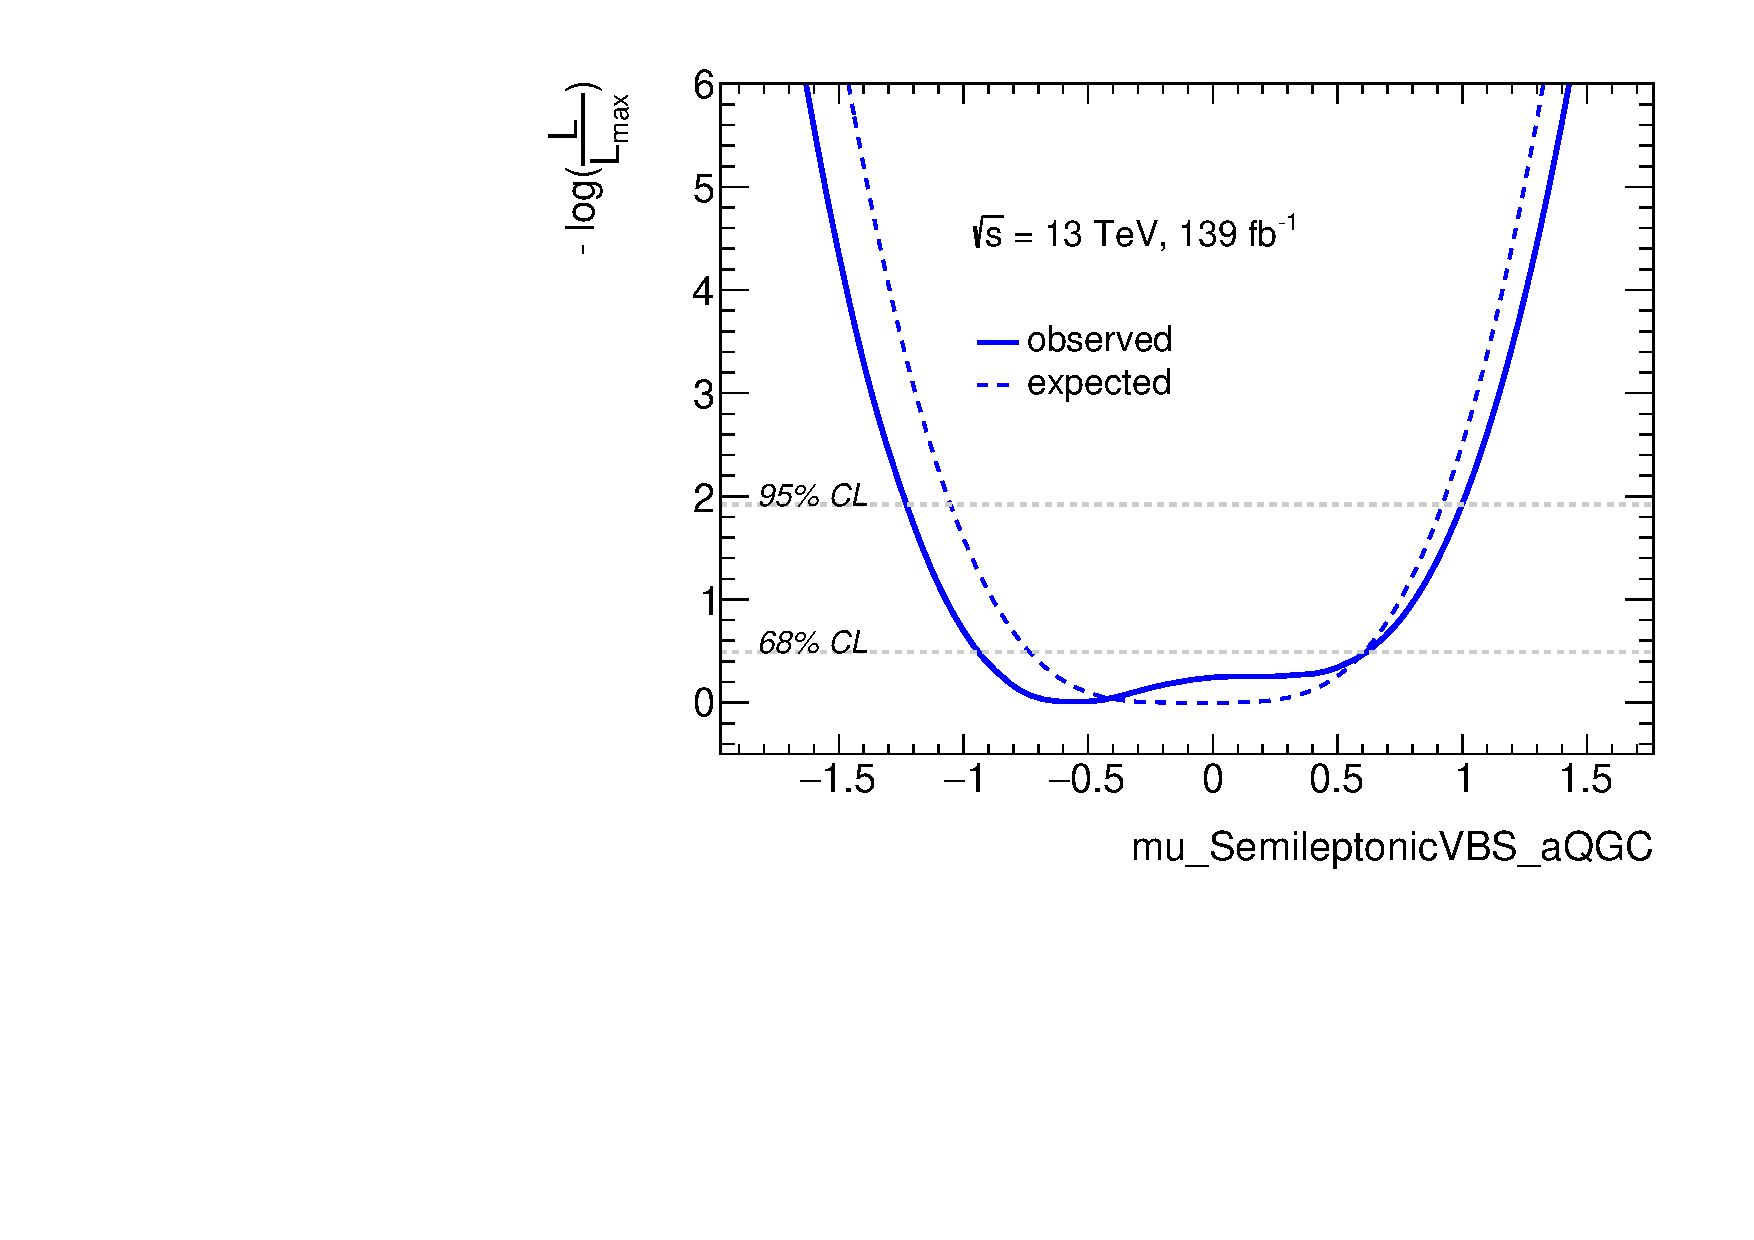
\includegraphics[width=0.32\textwidth]{figures/aQGC/profileFT01500}
    	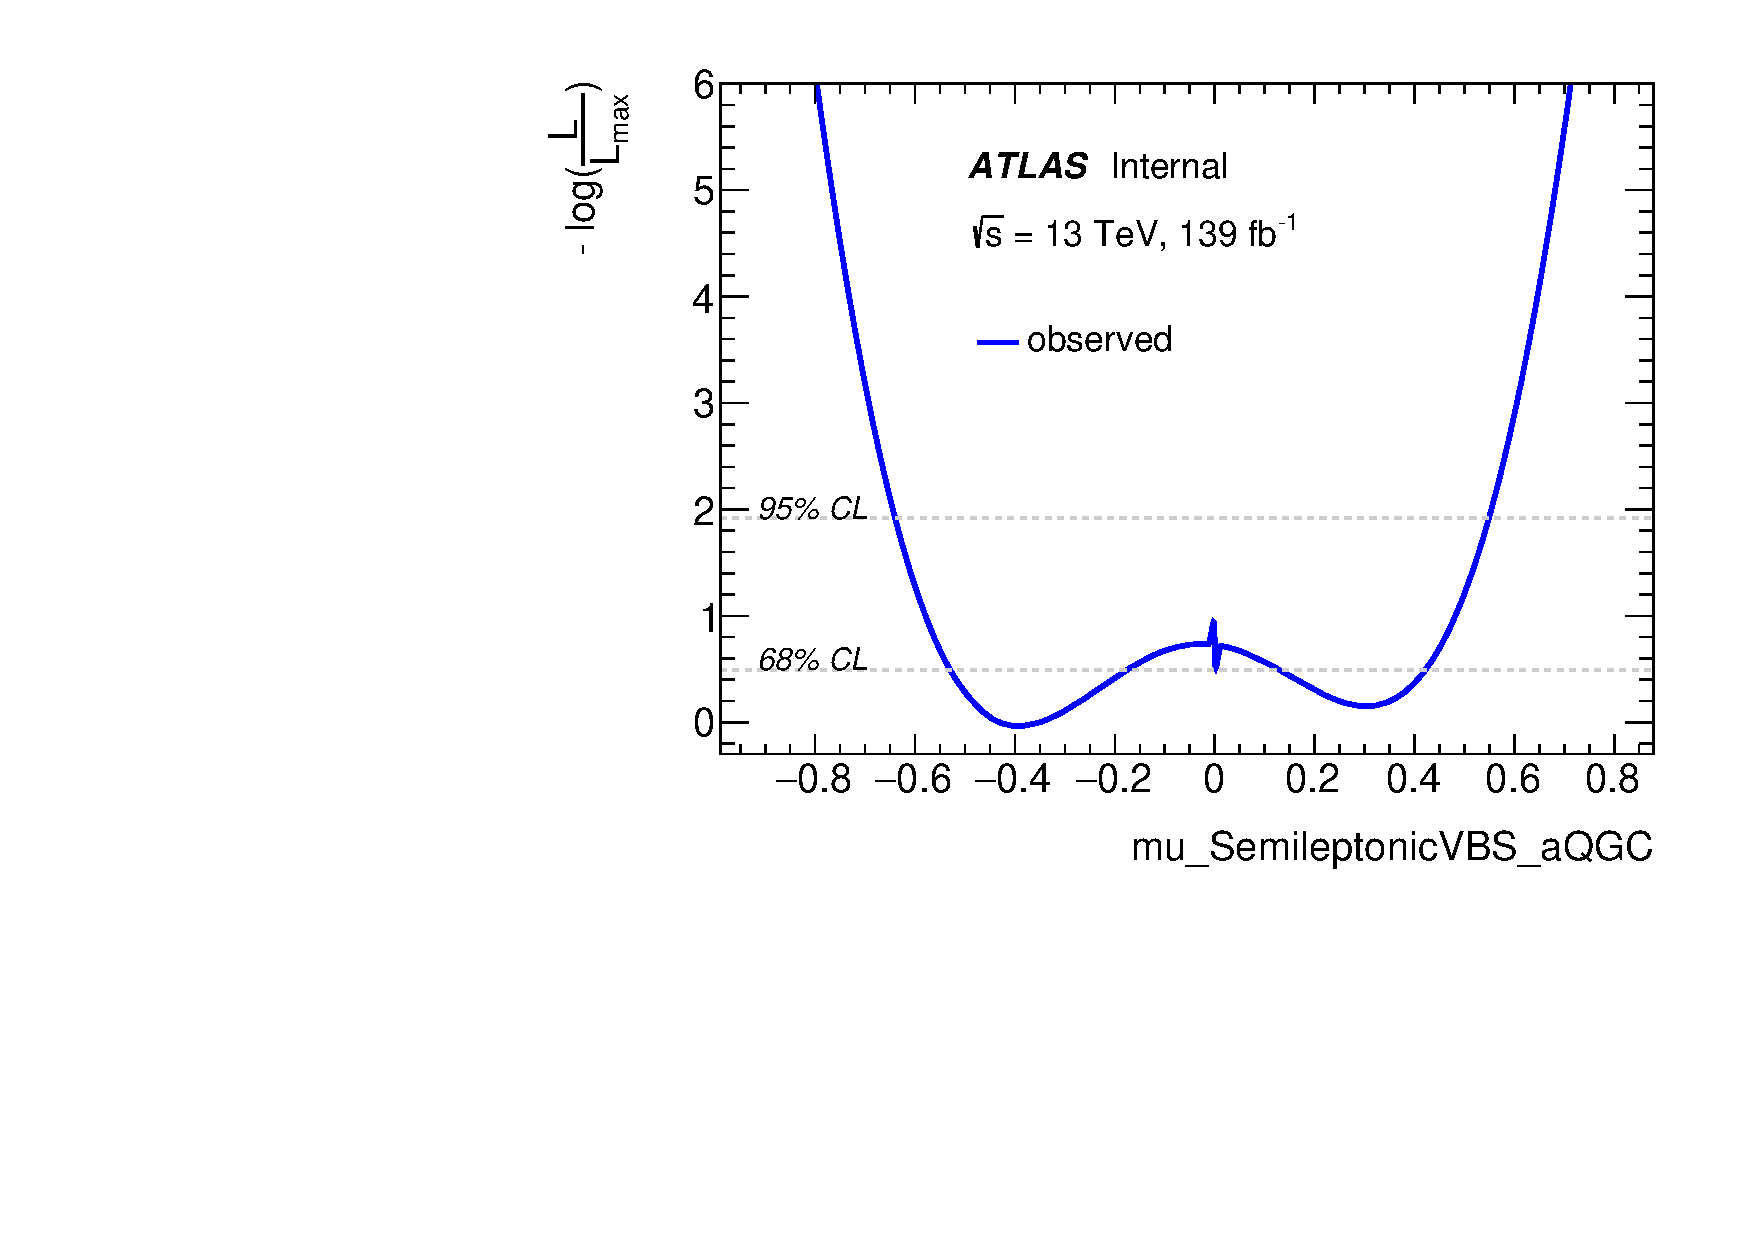
\includegraphics[width=0.32\textwidth]{figures/aQGC/profileFT02000}
    	%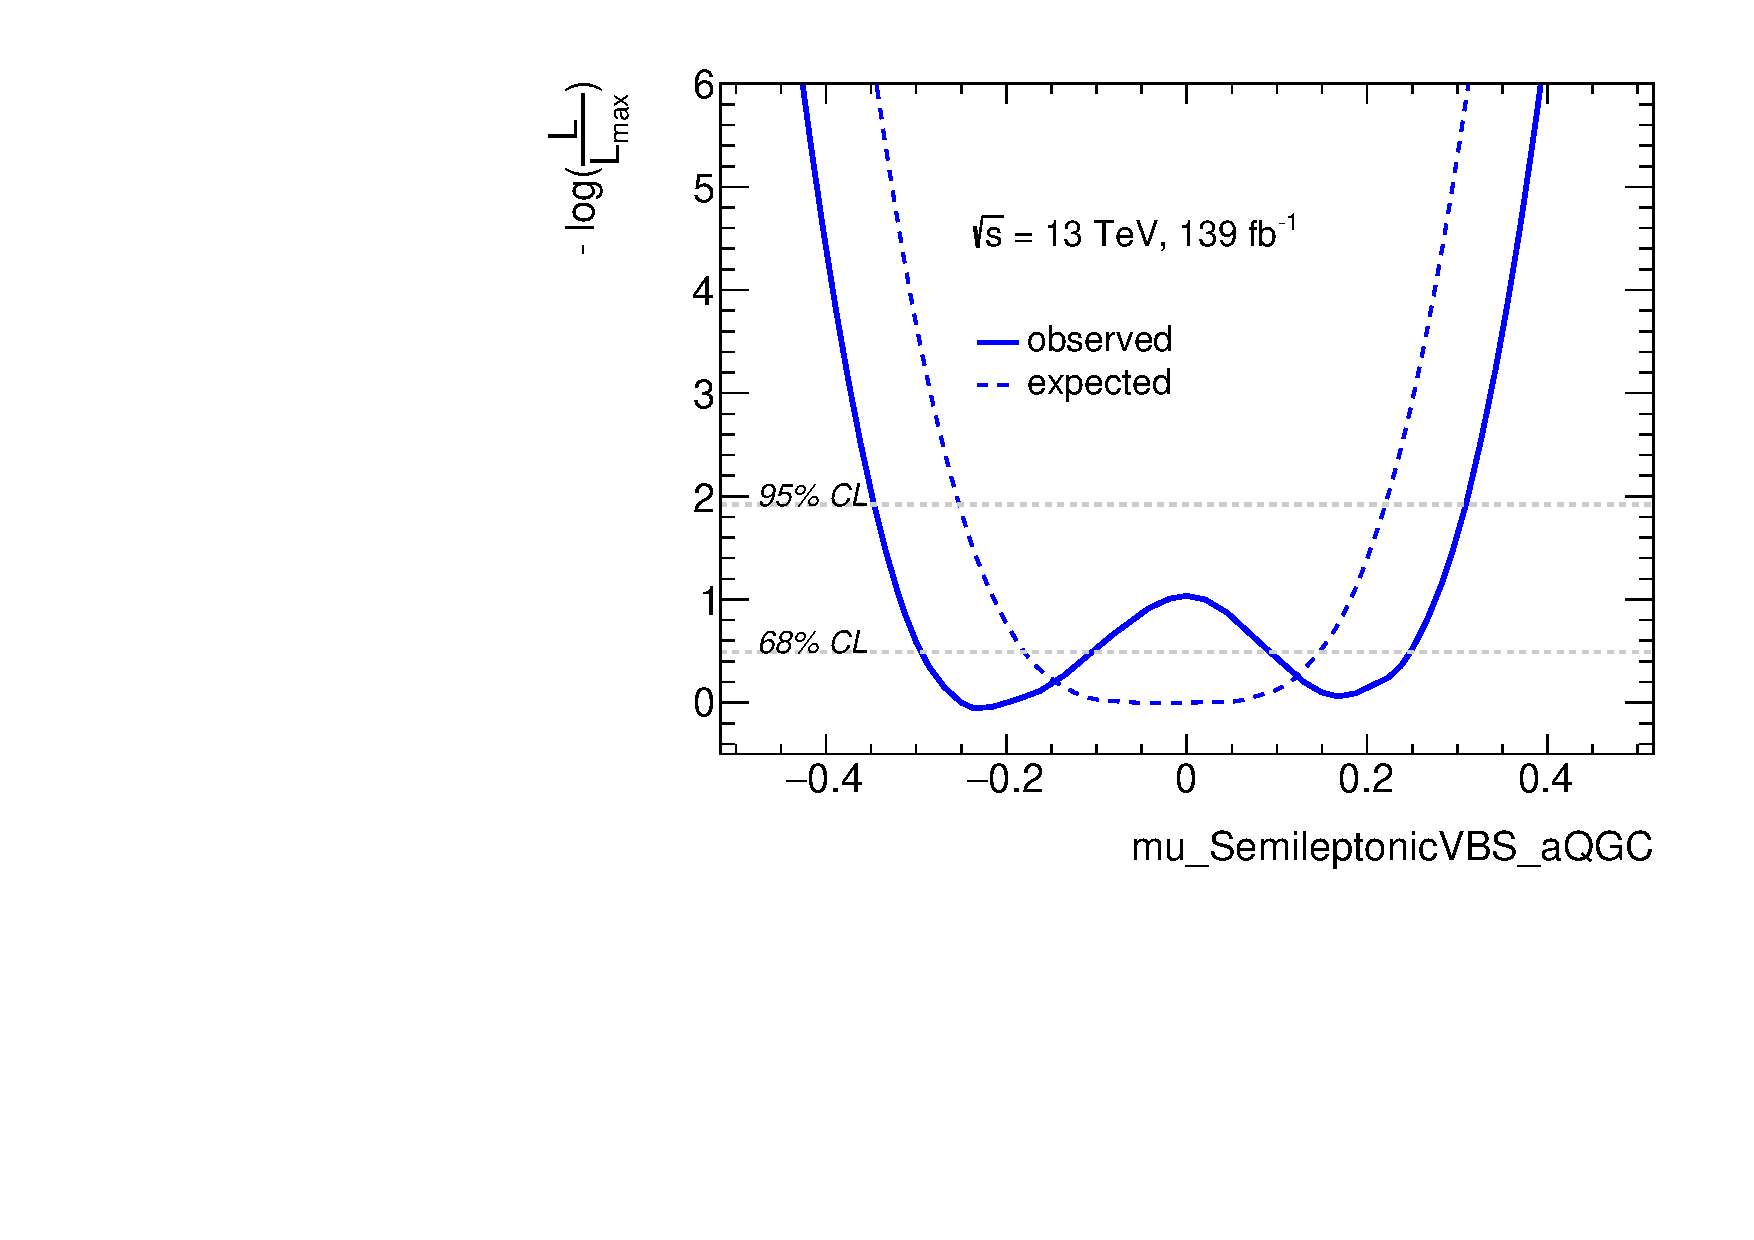
\includegraphics[width=0.38\textwidth]{figures/aQGC/profileFT03000}
        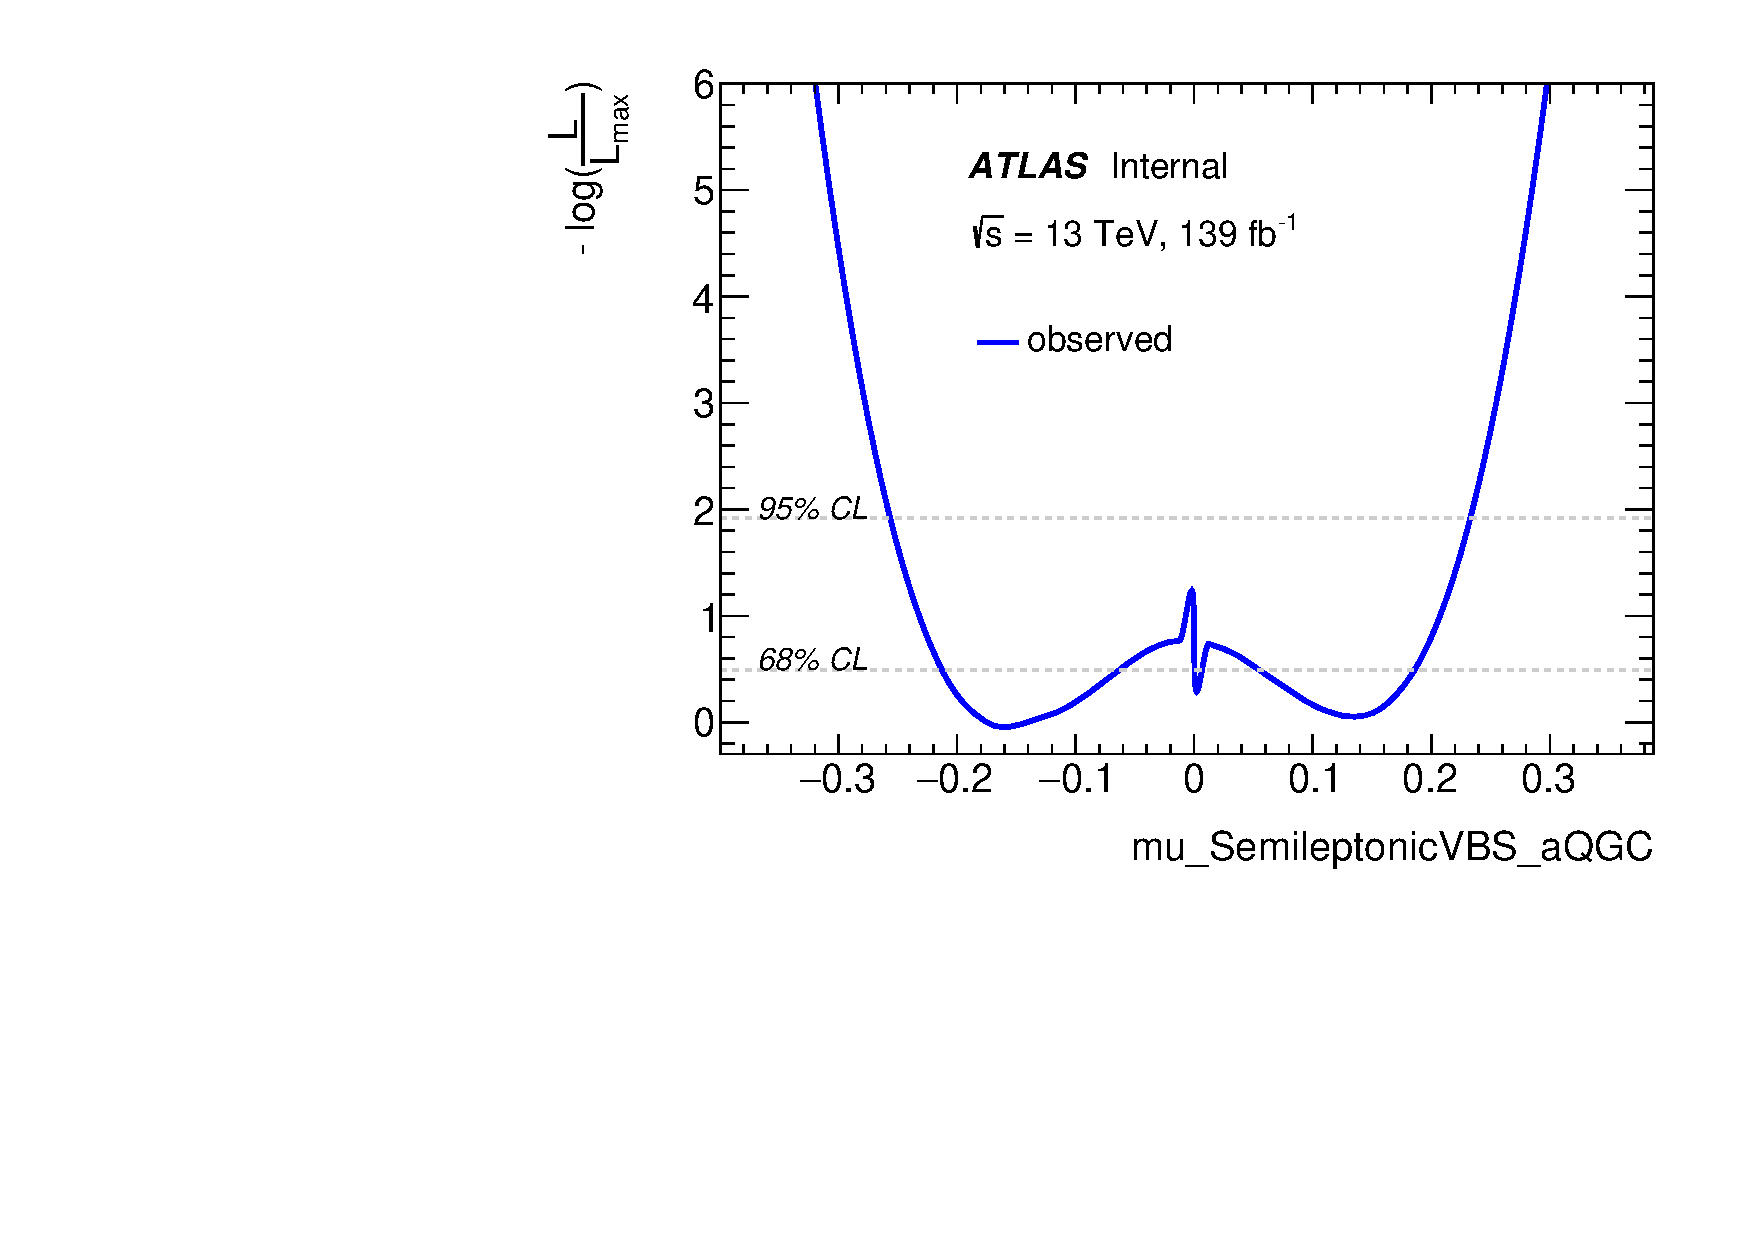
\includegraphics[width=0.32\textwidth]{figures/aQGC/profileFT0inf}
        \caption{The observed log-likelihood curves of FT0 Wilson coefficient where the clipping energy is 1.5~TeV (left), 2.0~TeV (middle), $\infty$ (right).}
        \label{fig:ProfileLL}
\end{figure}
\begin{figure}[ht]
    \centering
    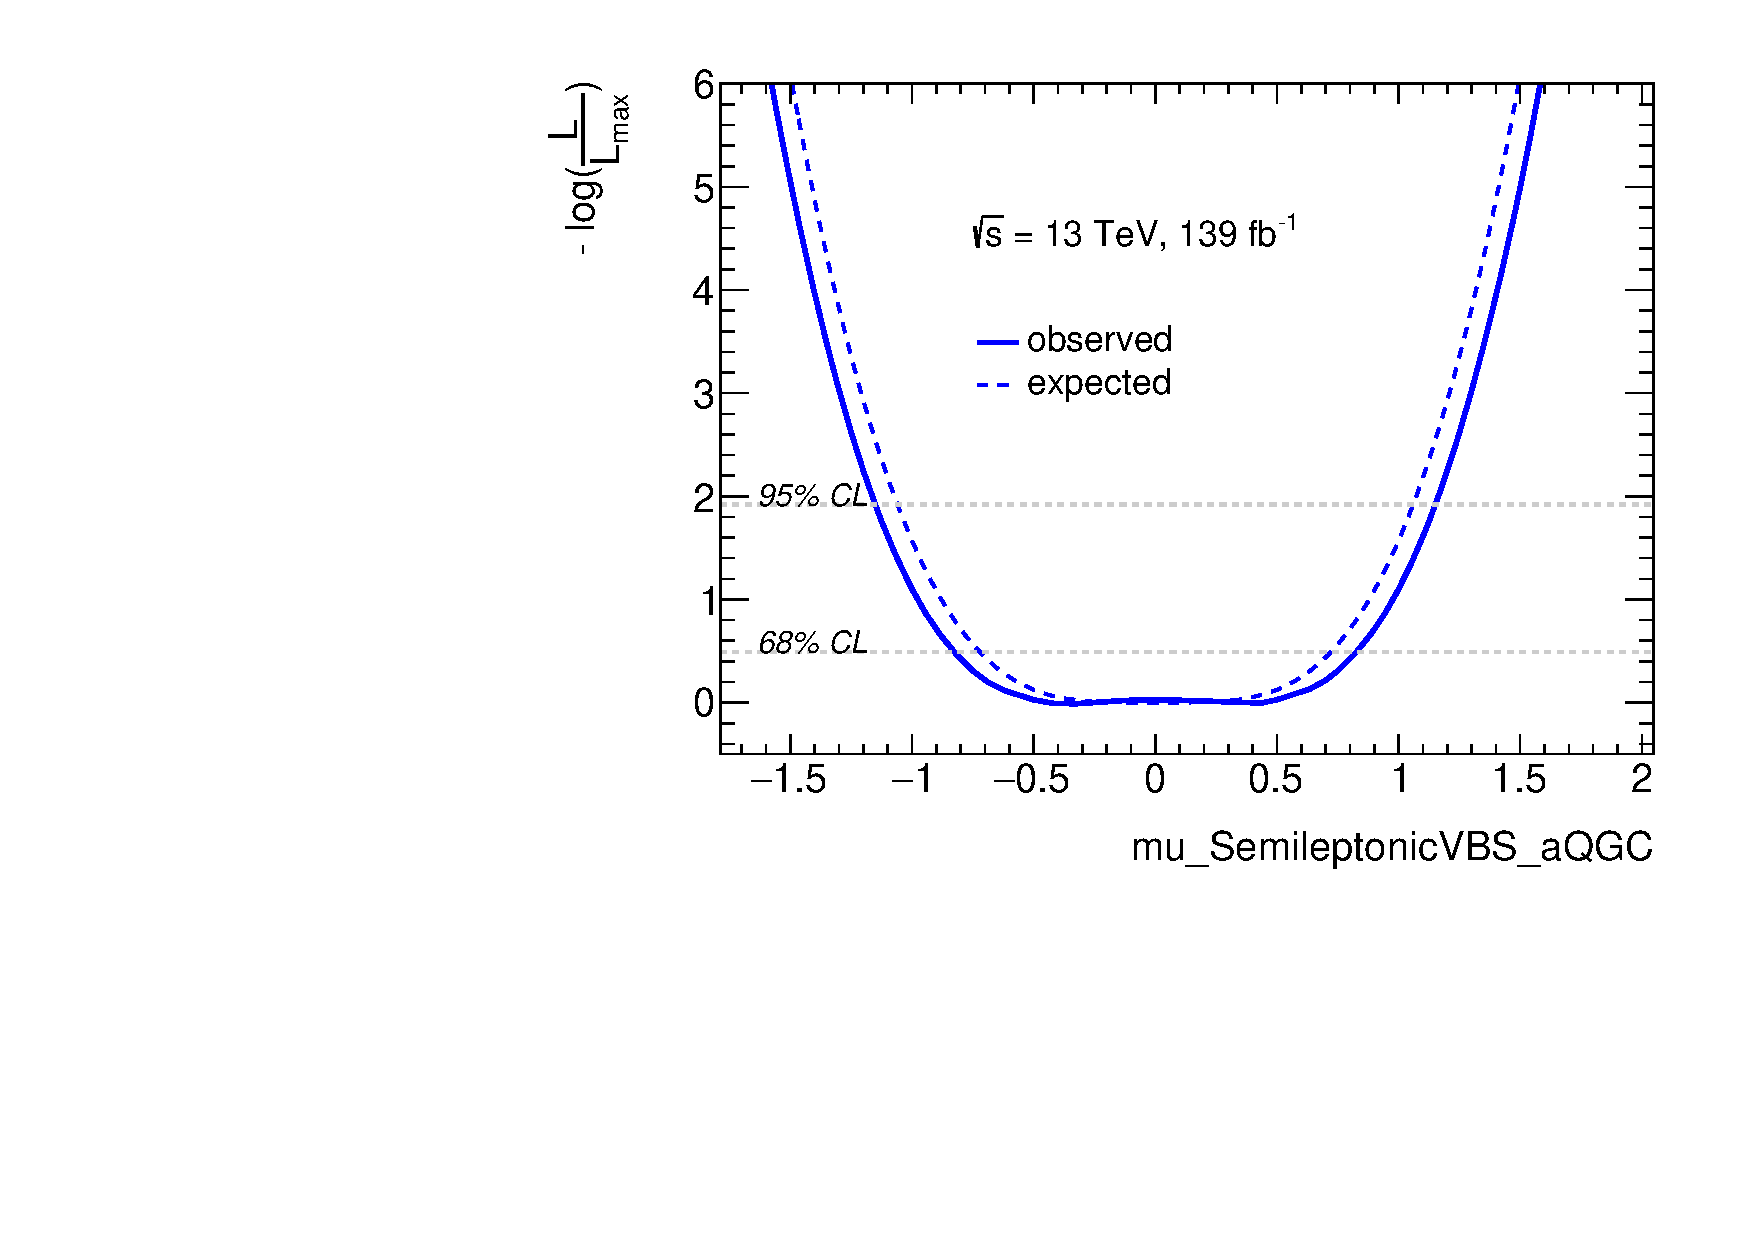
\includegraphics[width=0.32\textwidth]{figures/aQGC/profileFT11500}
    	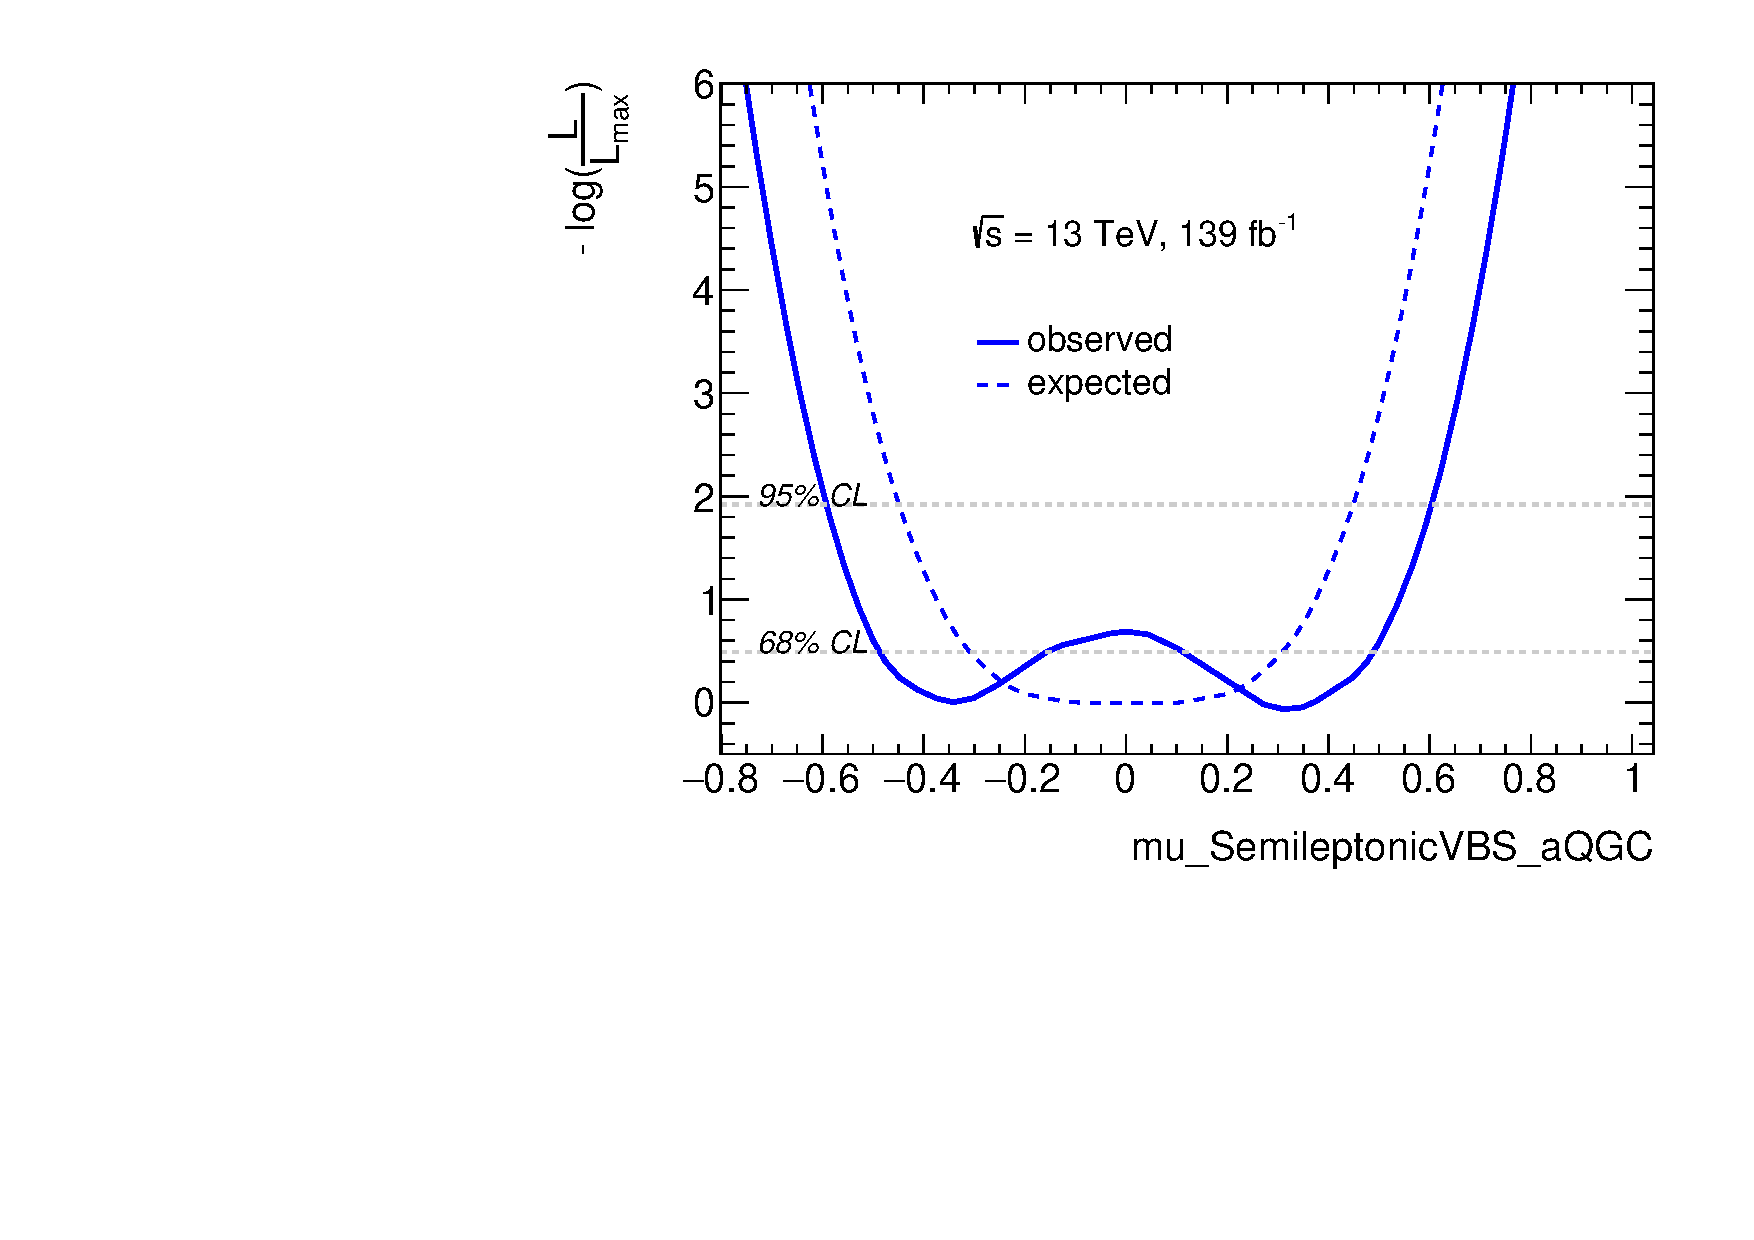
\includegraphics[width=0.32\textwidth]{figures/aQGC/profileFT12000}
    	%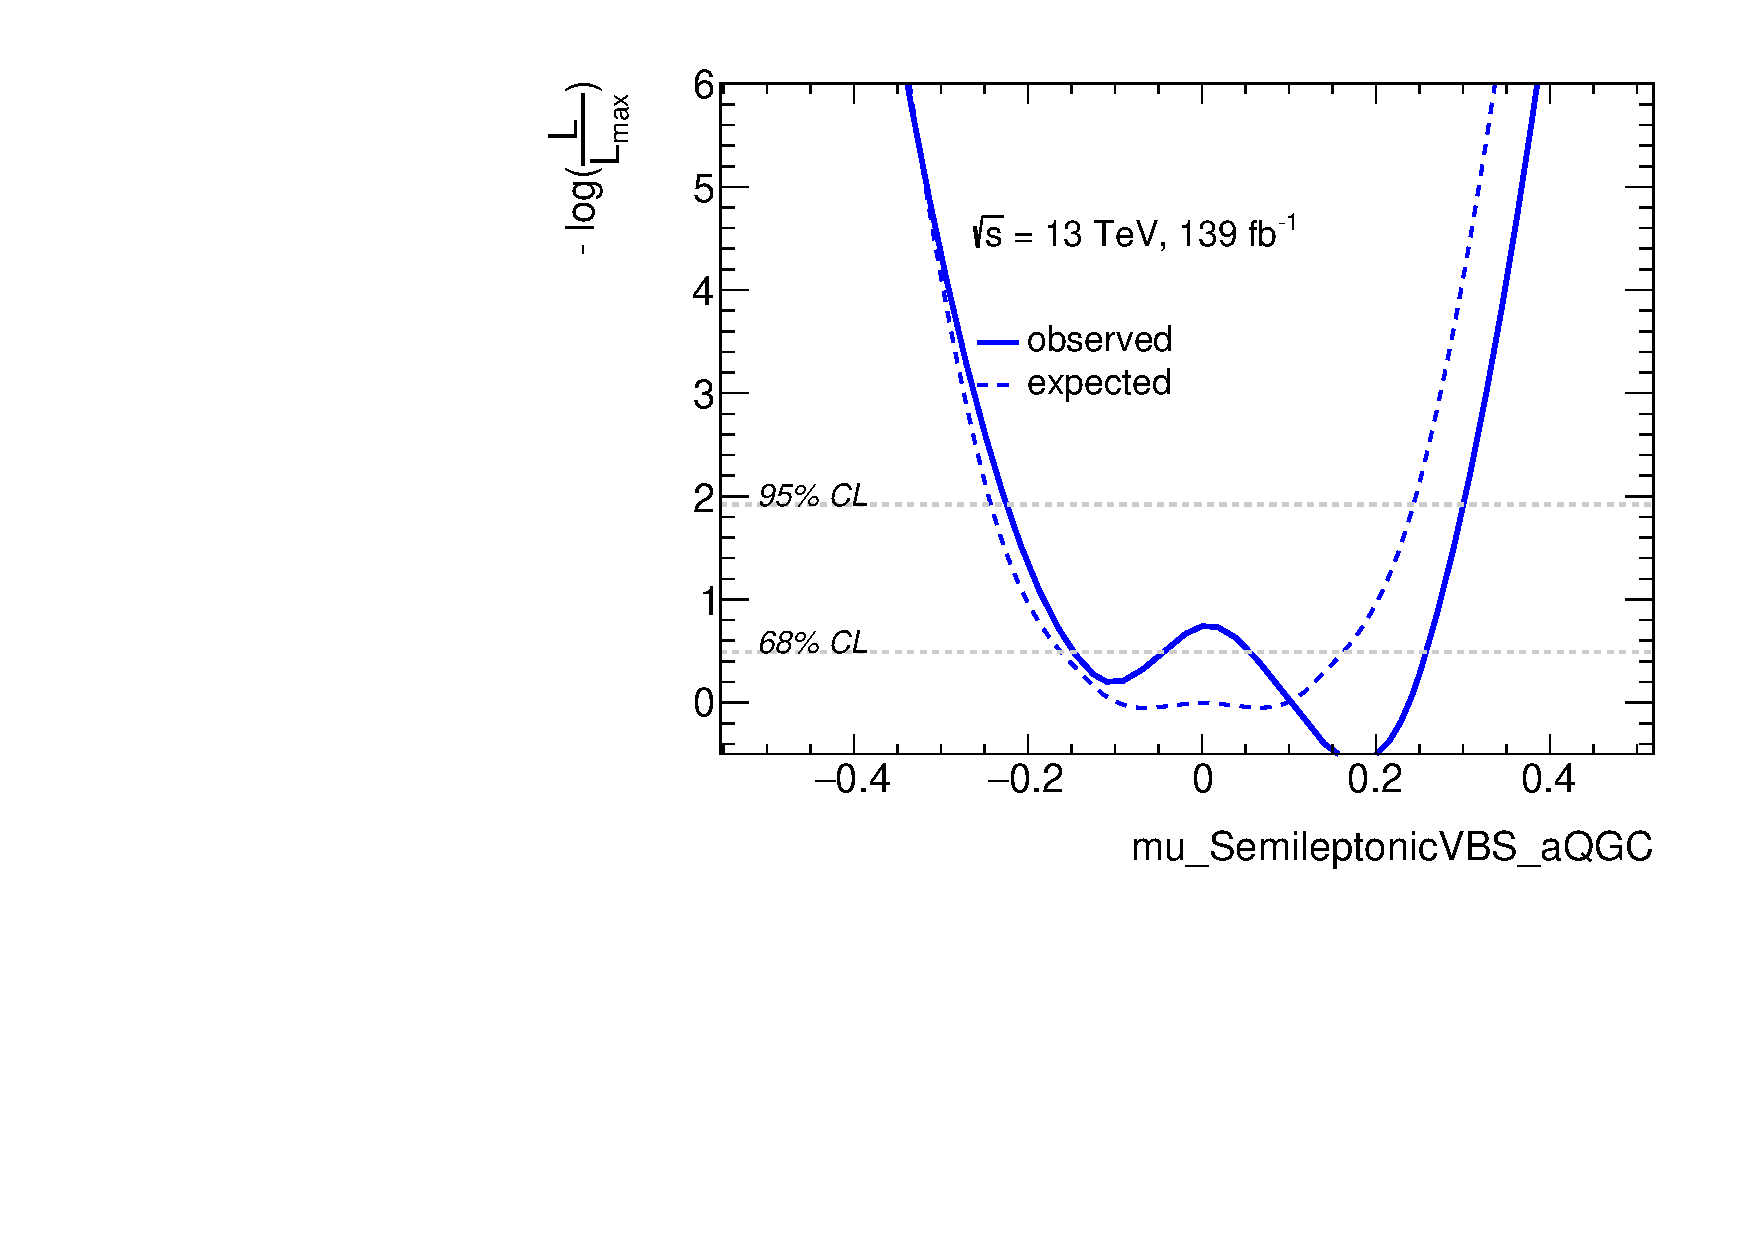
\includegraphics[width=0.38\textwidth]{figures/aQGC/profileFT13000}
        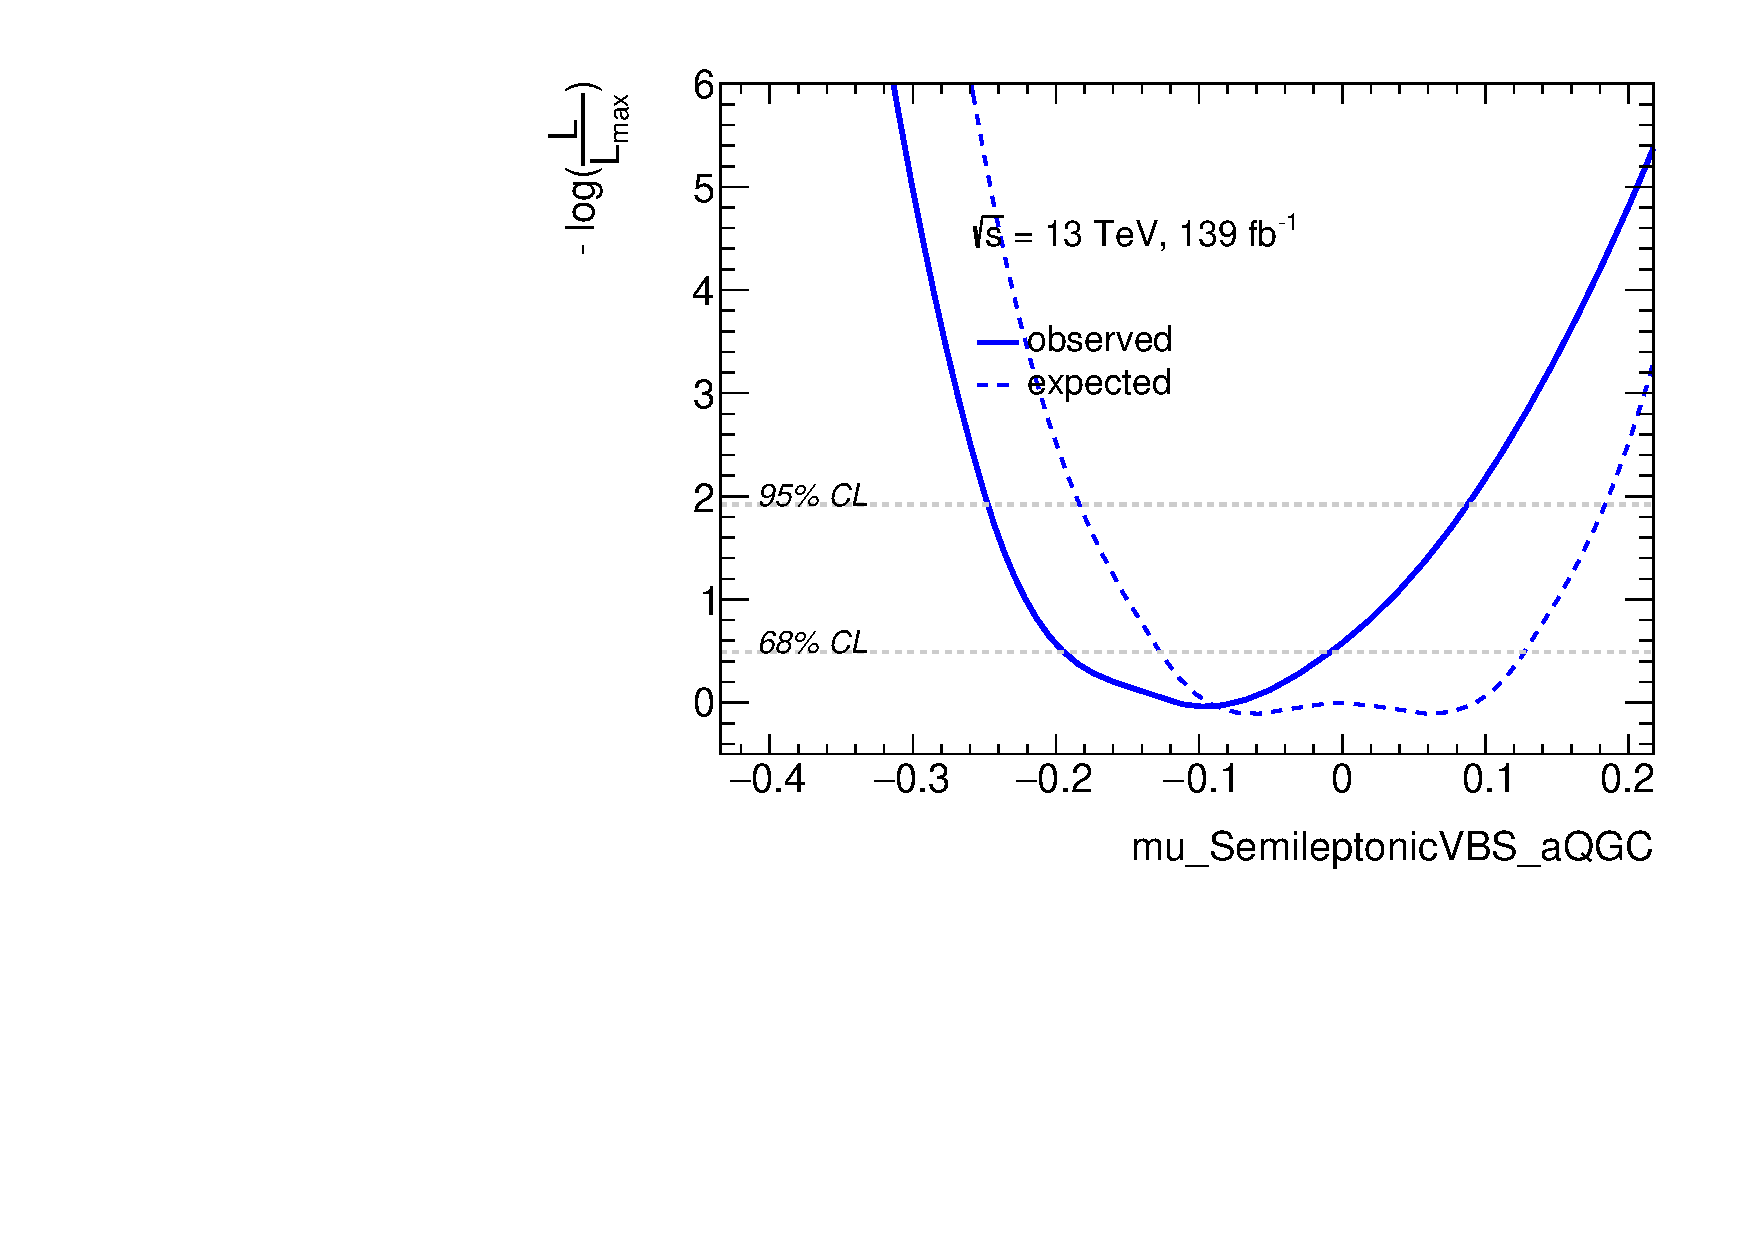
\includegraphics[width=0.32\textwidth]{figures/aQGC/profileFT1inf}
        \caption{The observed log-likelihood curves of FT1 Wilson coefficient where the clipping energy is 1.5~TeV (left), 2.0~TeV (middle), $\infty$ (right).}
        \label{fig:ProfileLL}
\end{figure}
\begin{figure}[ht]
    \centering
    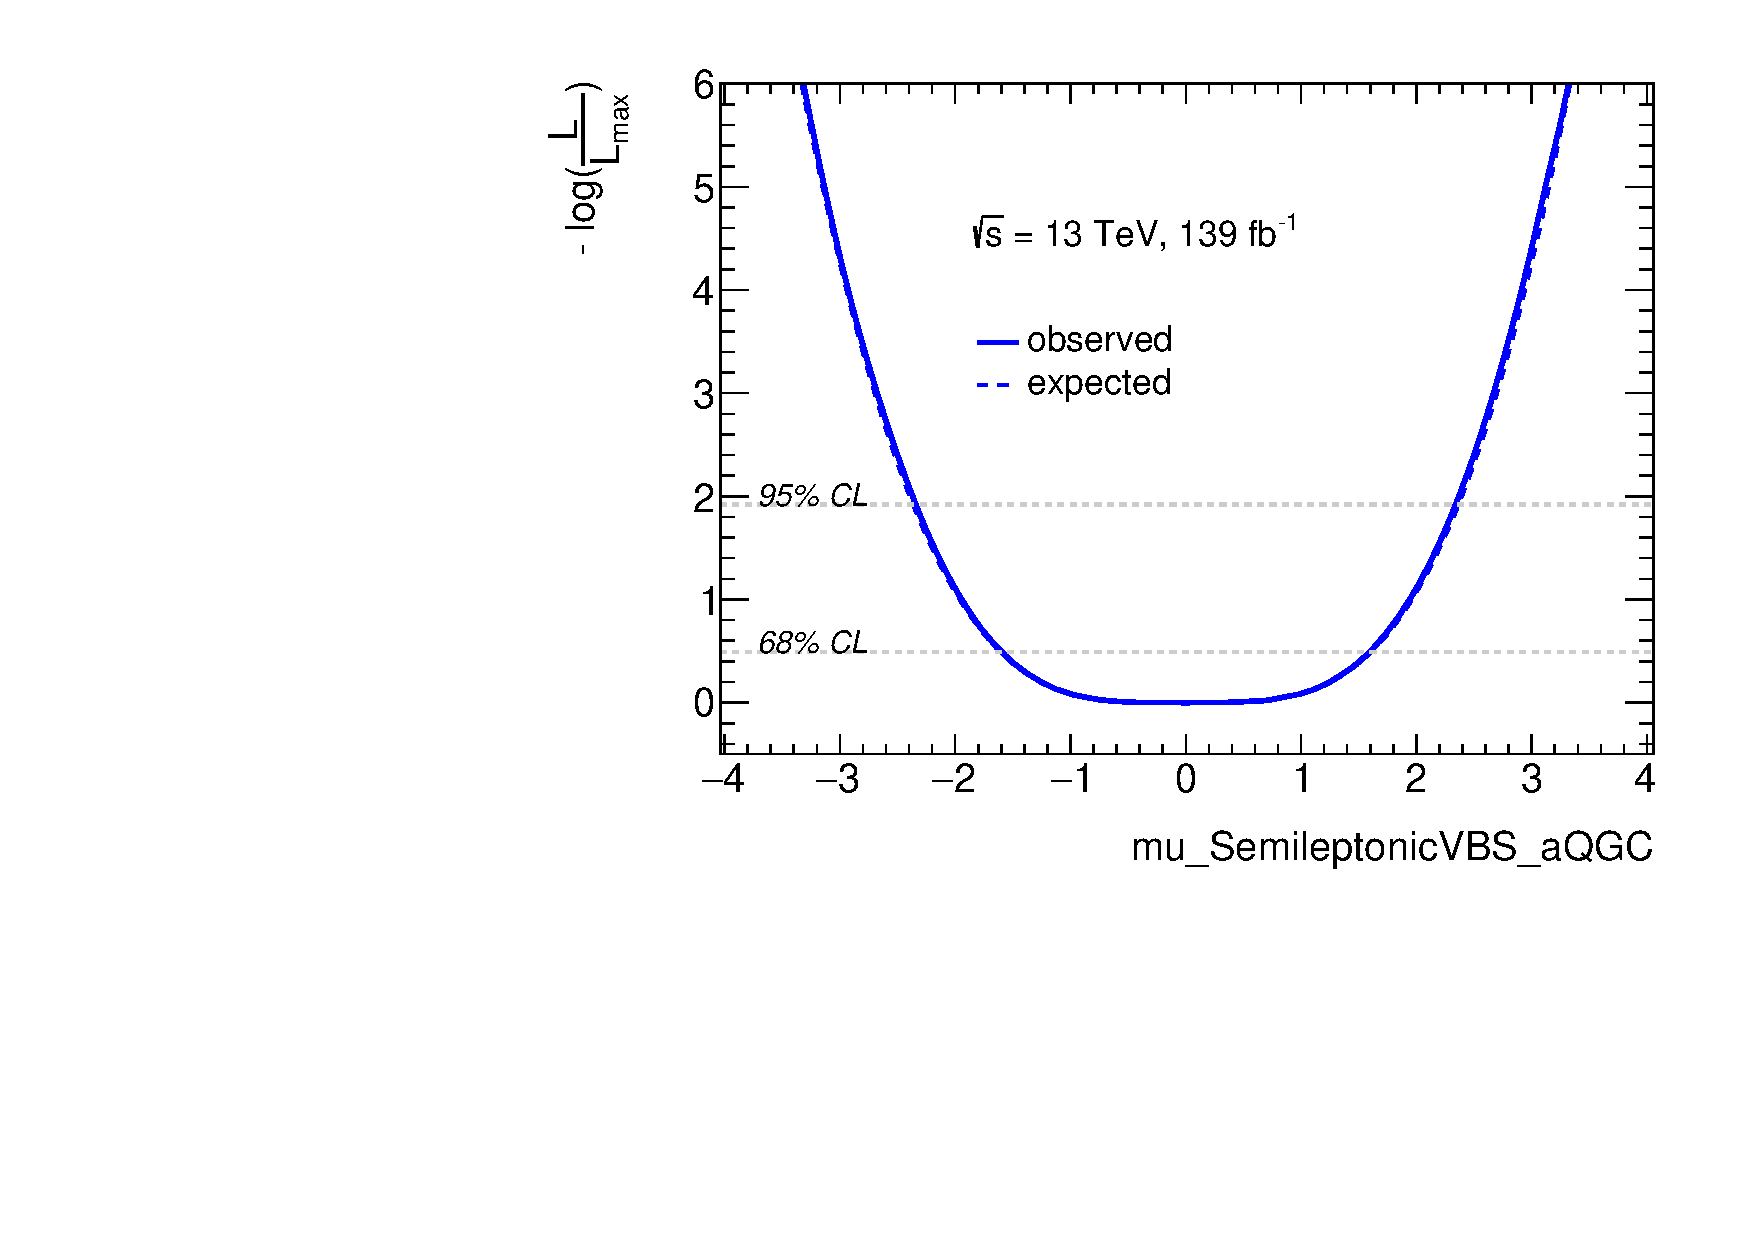
\includegraphics[width=0.32\textwidth]{figures/aQGC/profileFT21500}
    	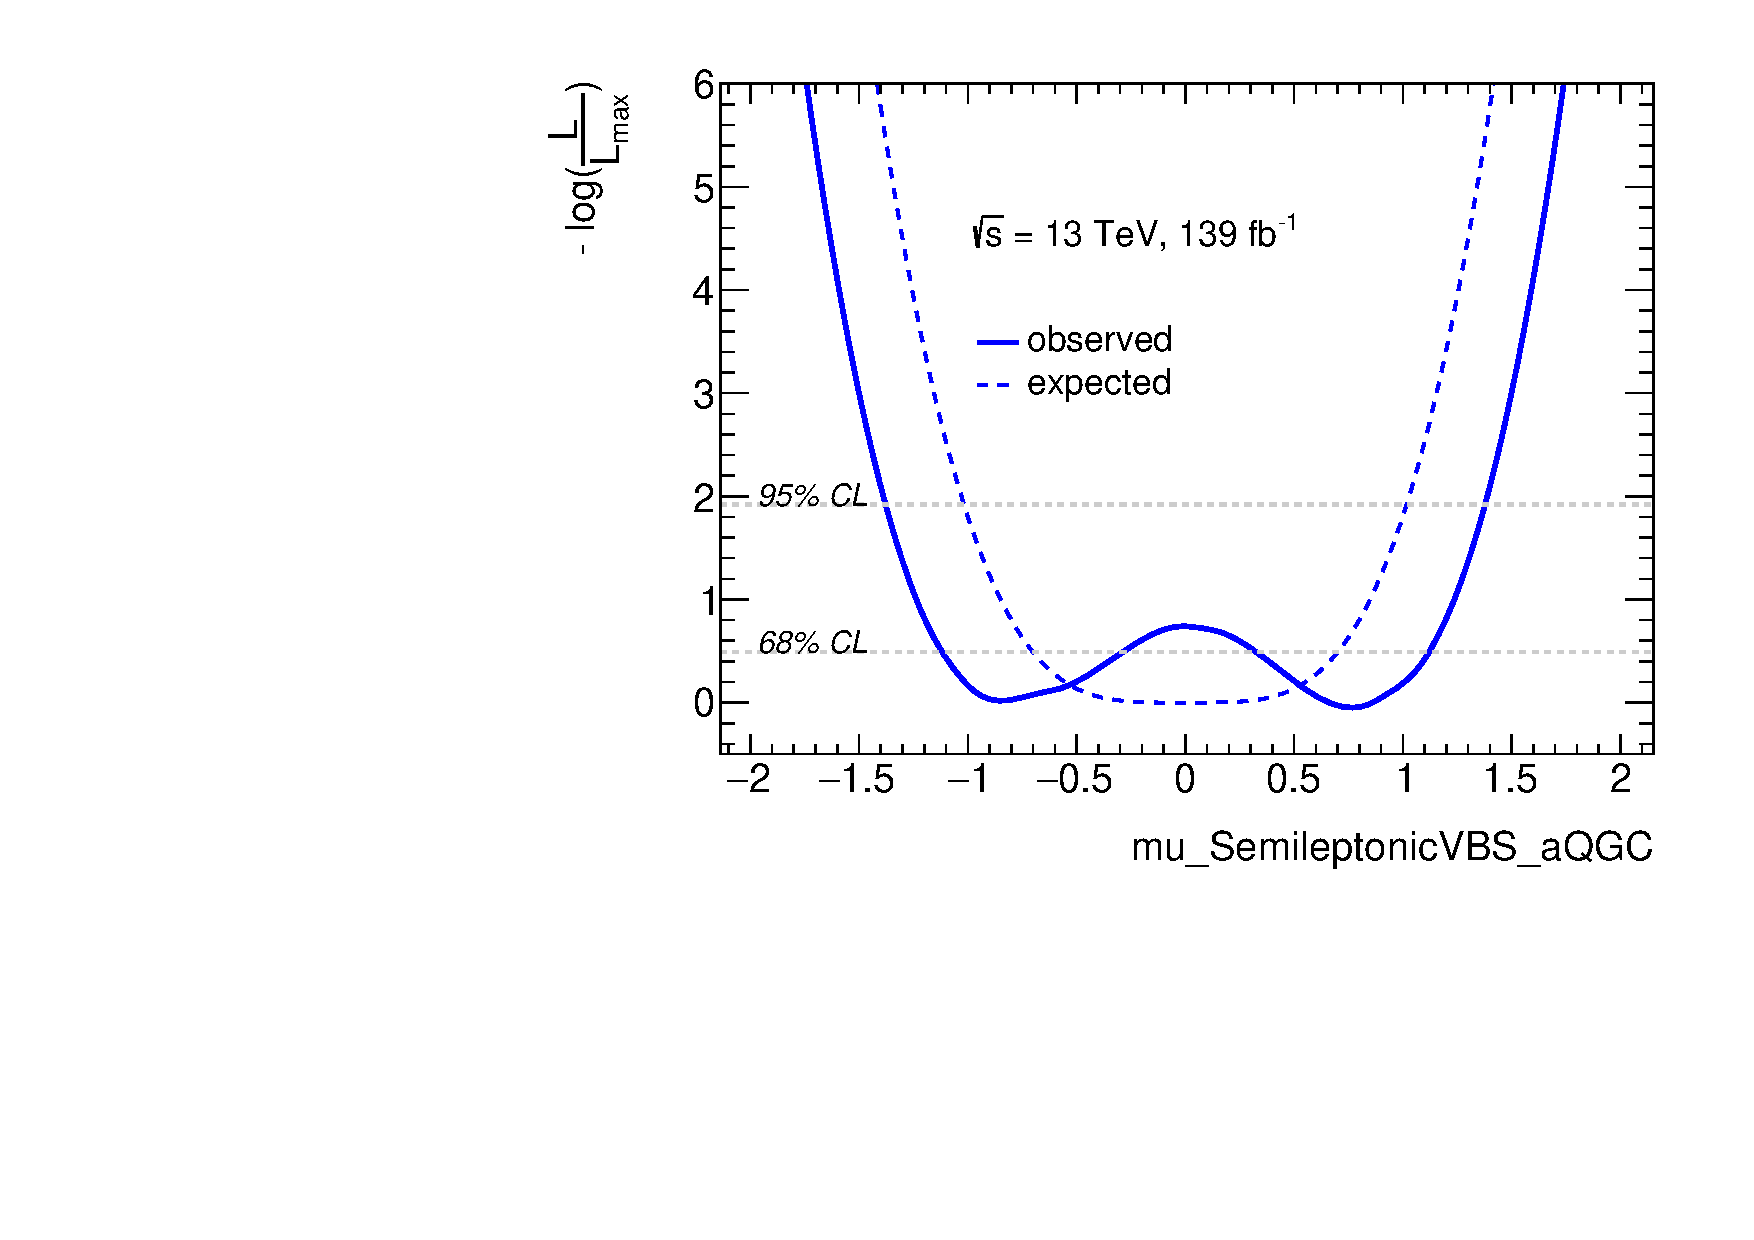
\includegraphics[width=0.32\textwidth]{figures/aQGC/profileFT22000}
    	%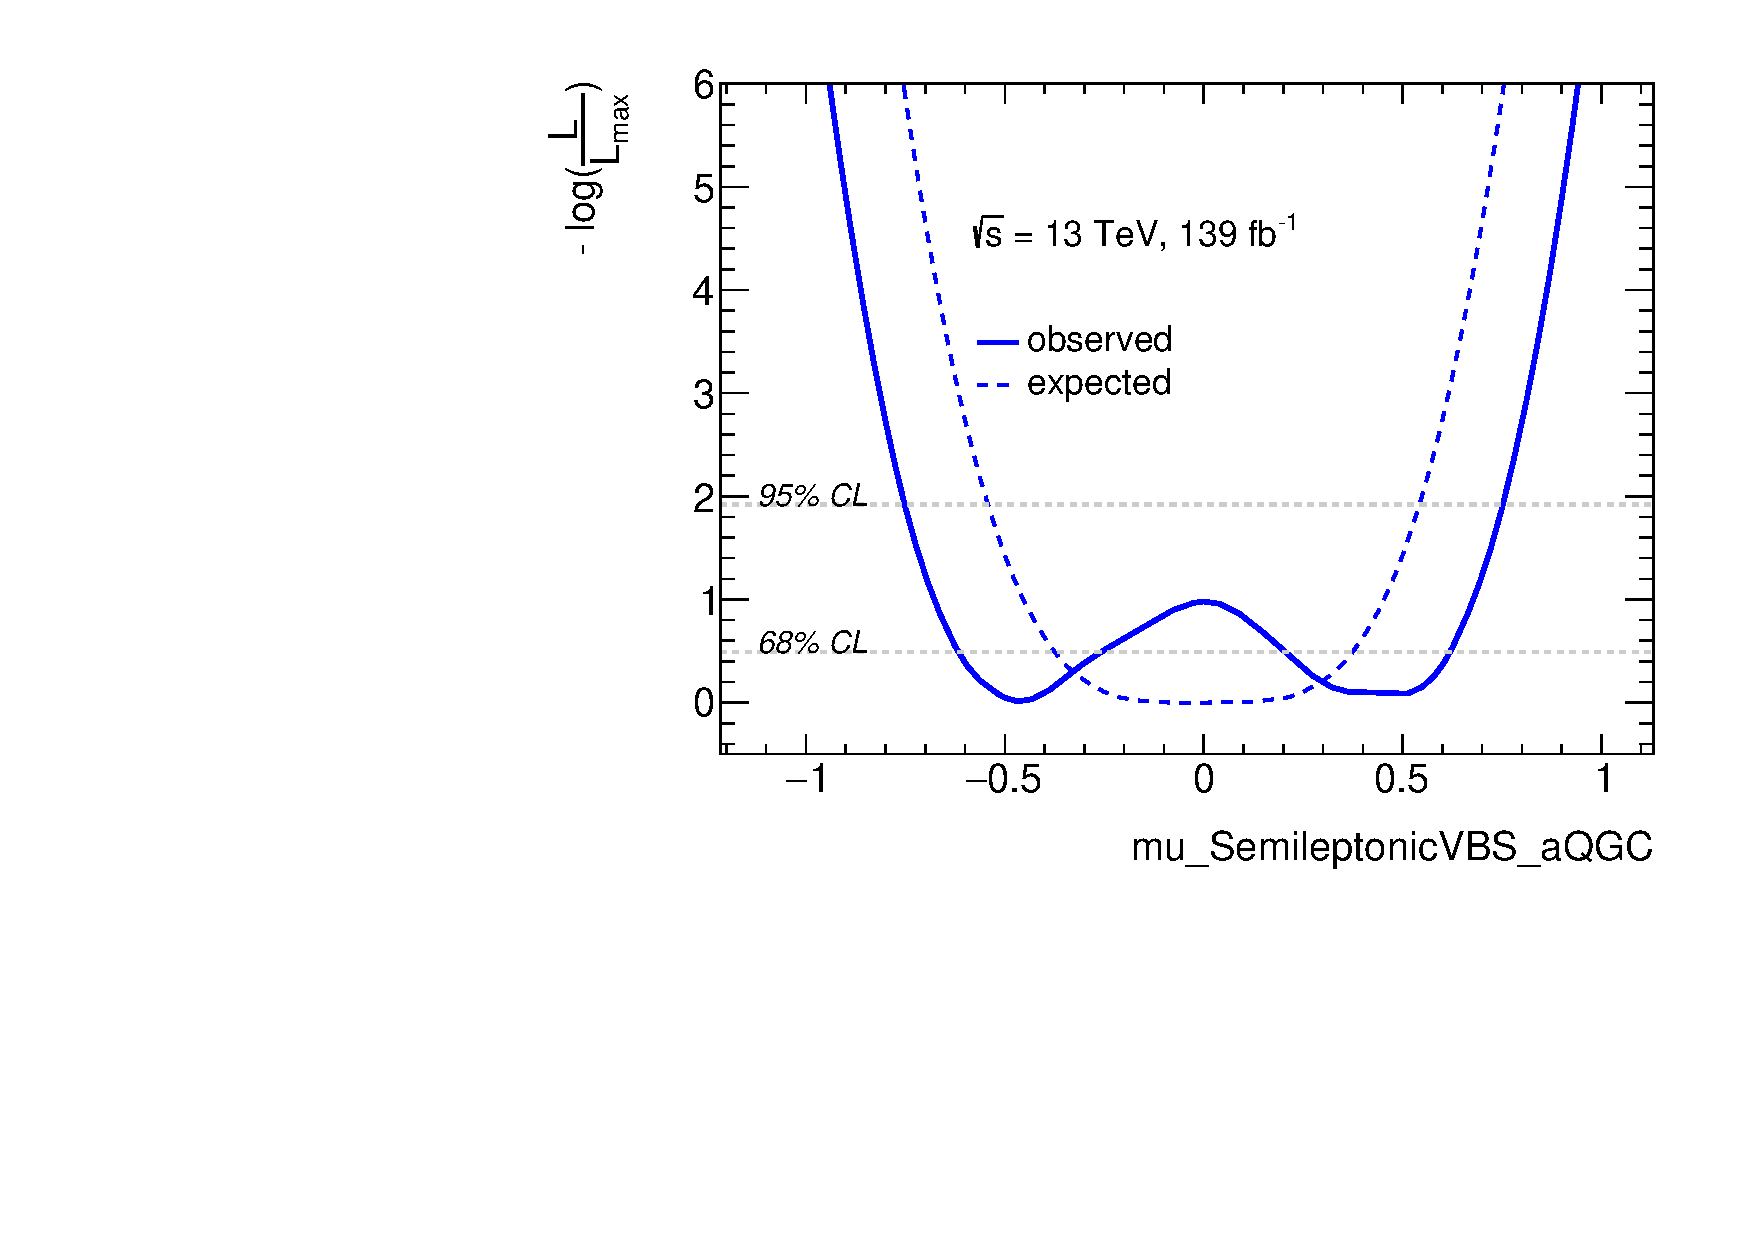
\includegraphics[width=0.38\textwidth]{figures/aQGC/profileFT23000}
        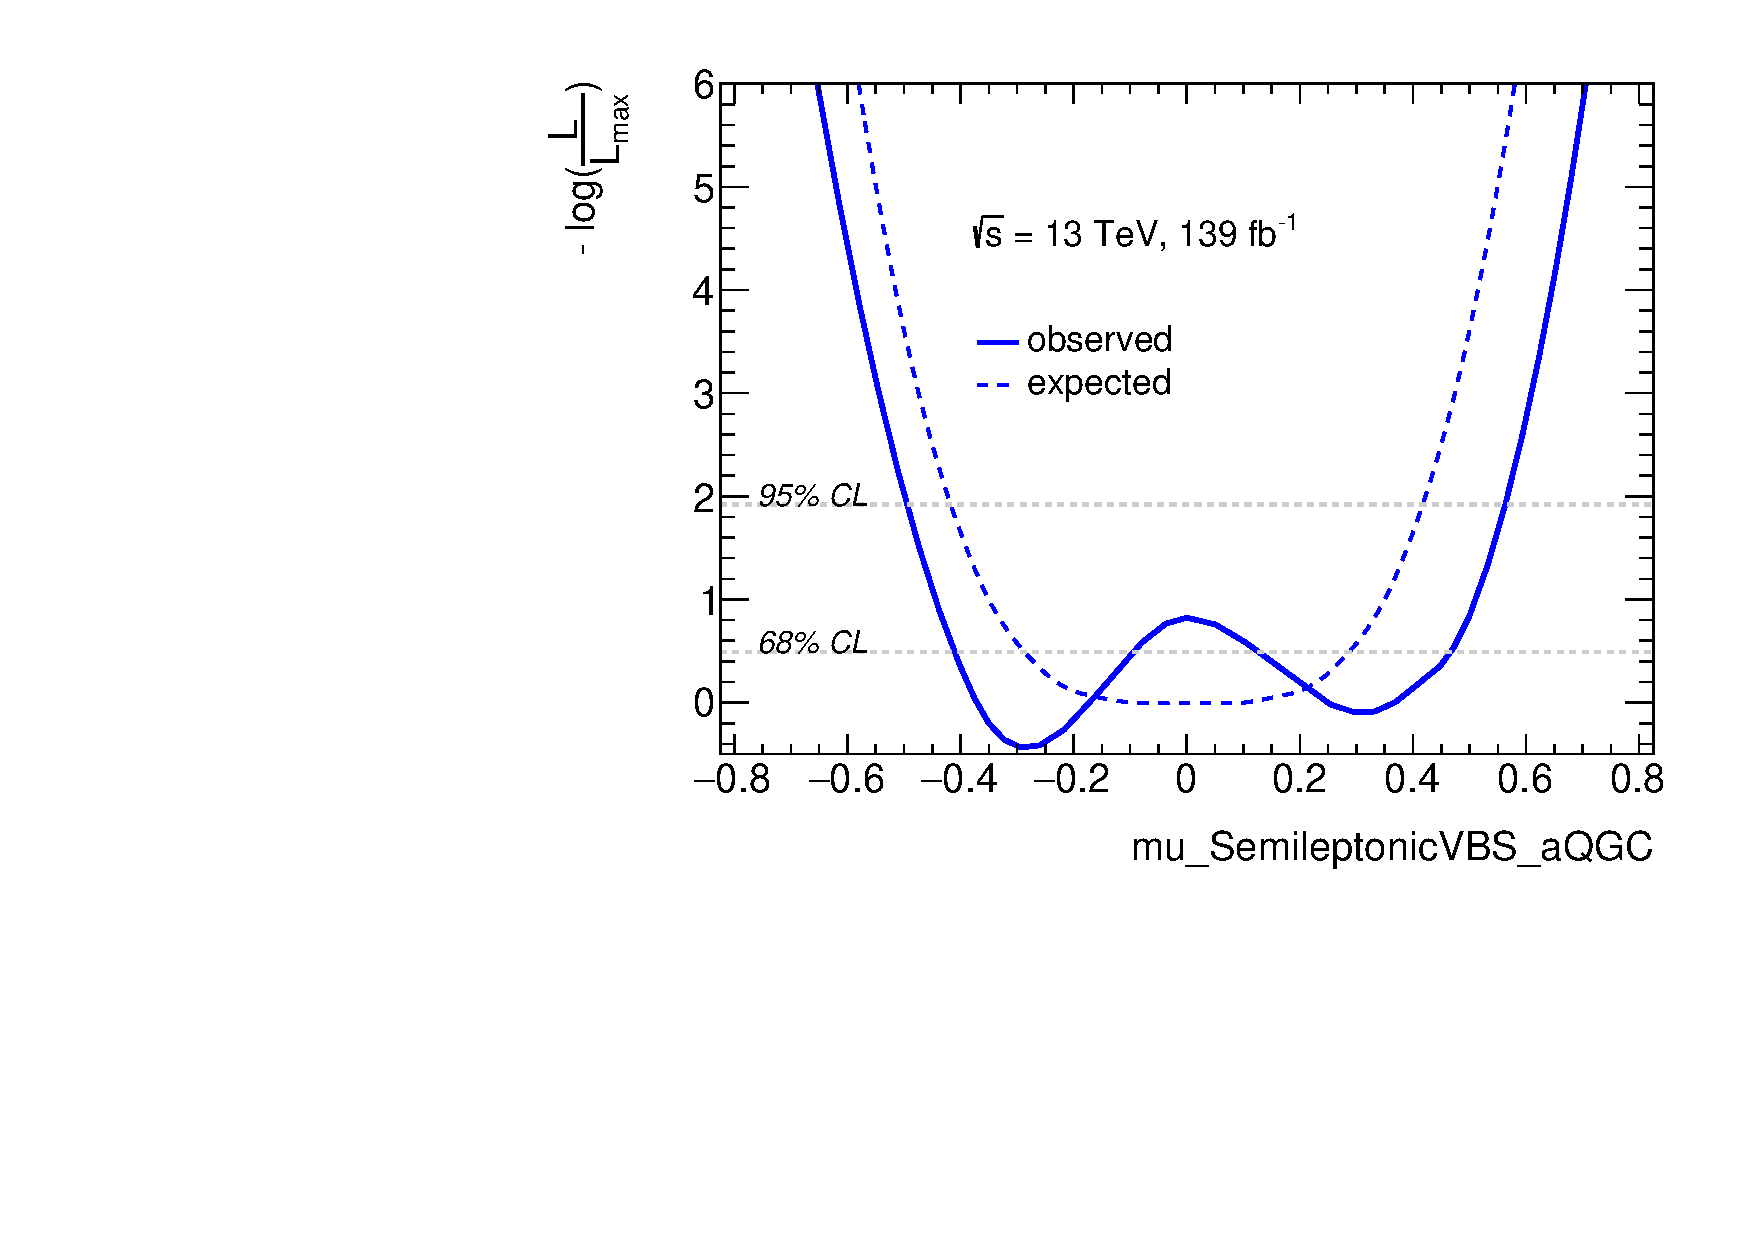
\includegraphics[width=0.32\textwidth]{figures/aQGC/profileFT2inf}
        \caption{The observed log-likelihood curves of FT2 Wilson coefficient where the clipping energy is 1.5~TeV (left), 2.0~TeV (middle), $\infty$ (right).}
        \label{fig:ProfileLL}
\end{figure}
\begin{figure}[ht]
    \centering
    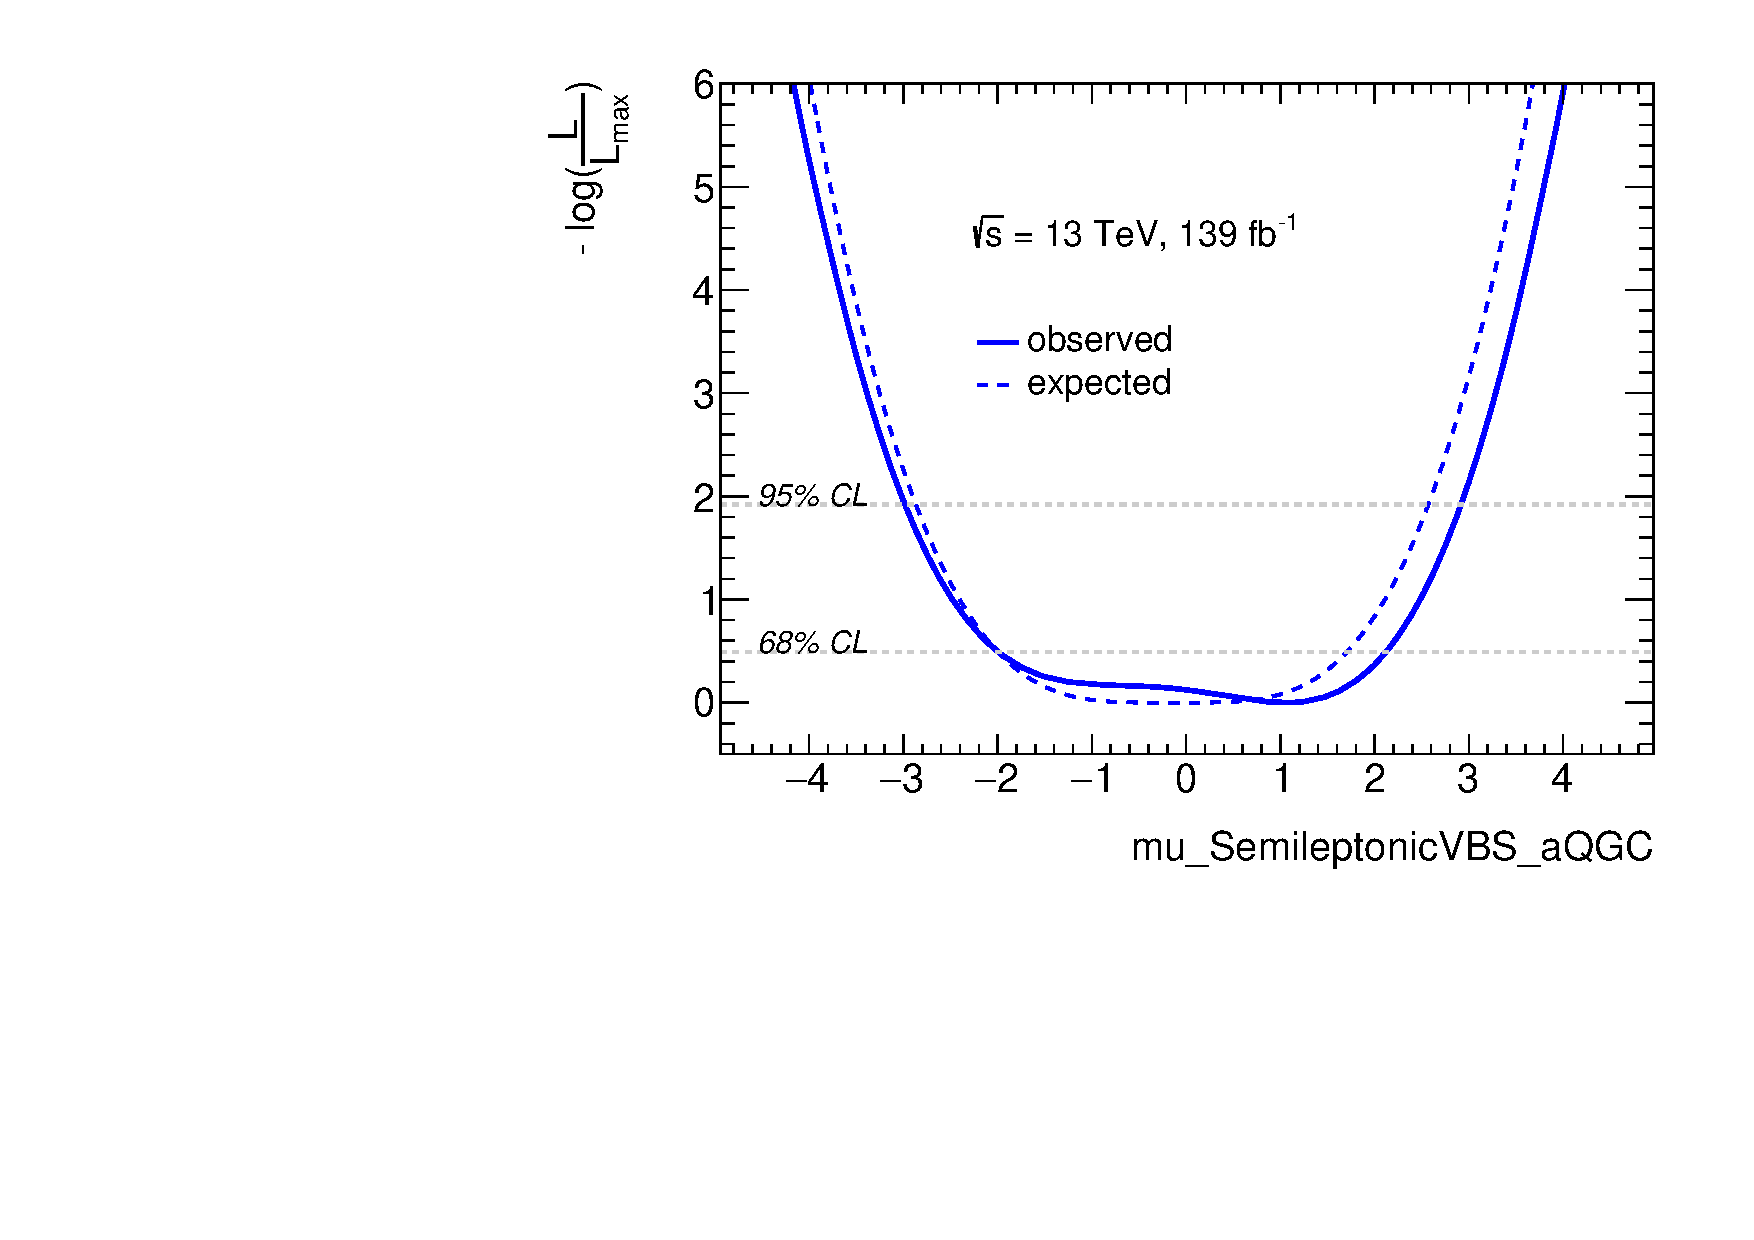
\includegraphics[width=0.32\textwidth]{figures/aQGC/profileFT51500}
    	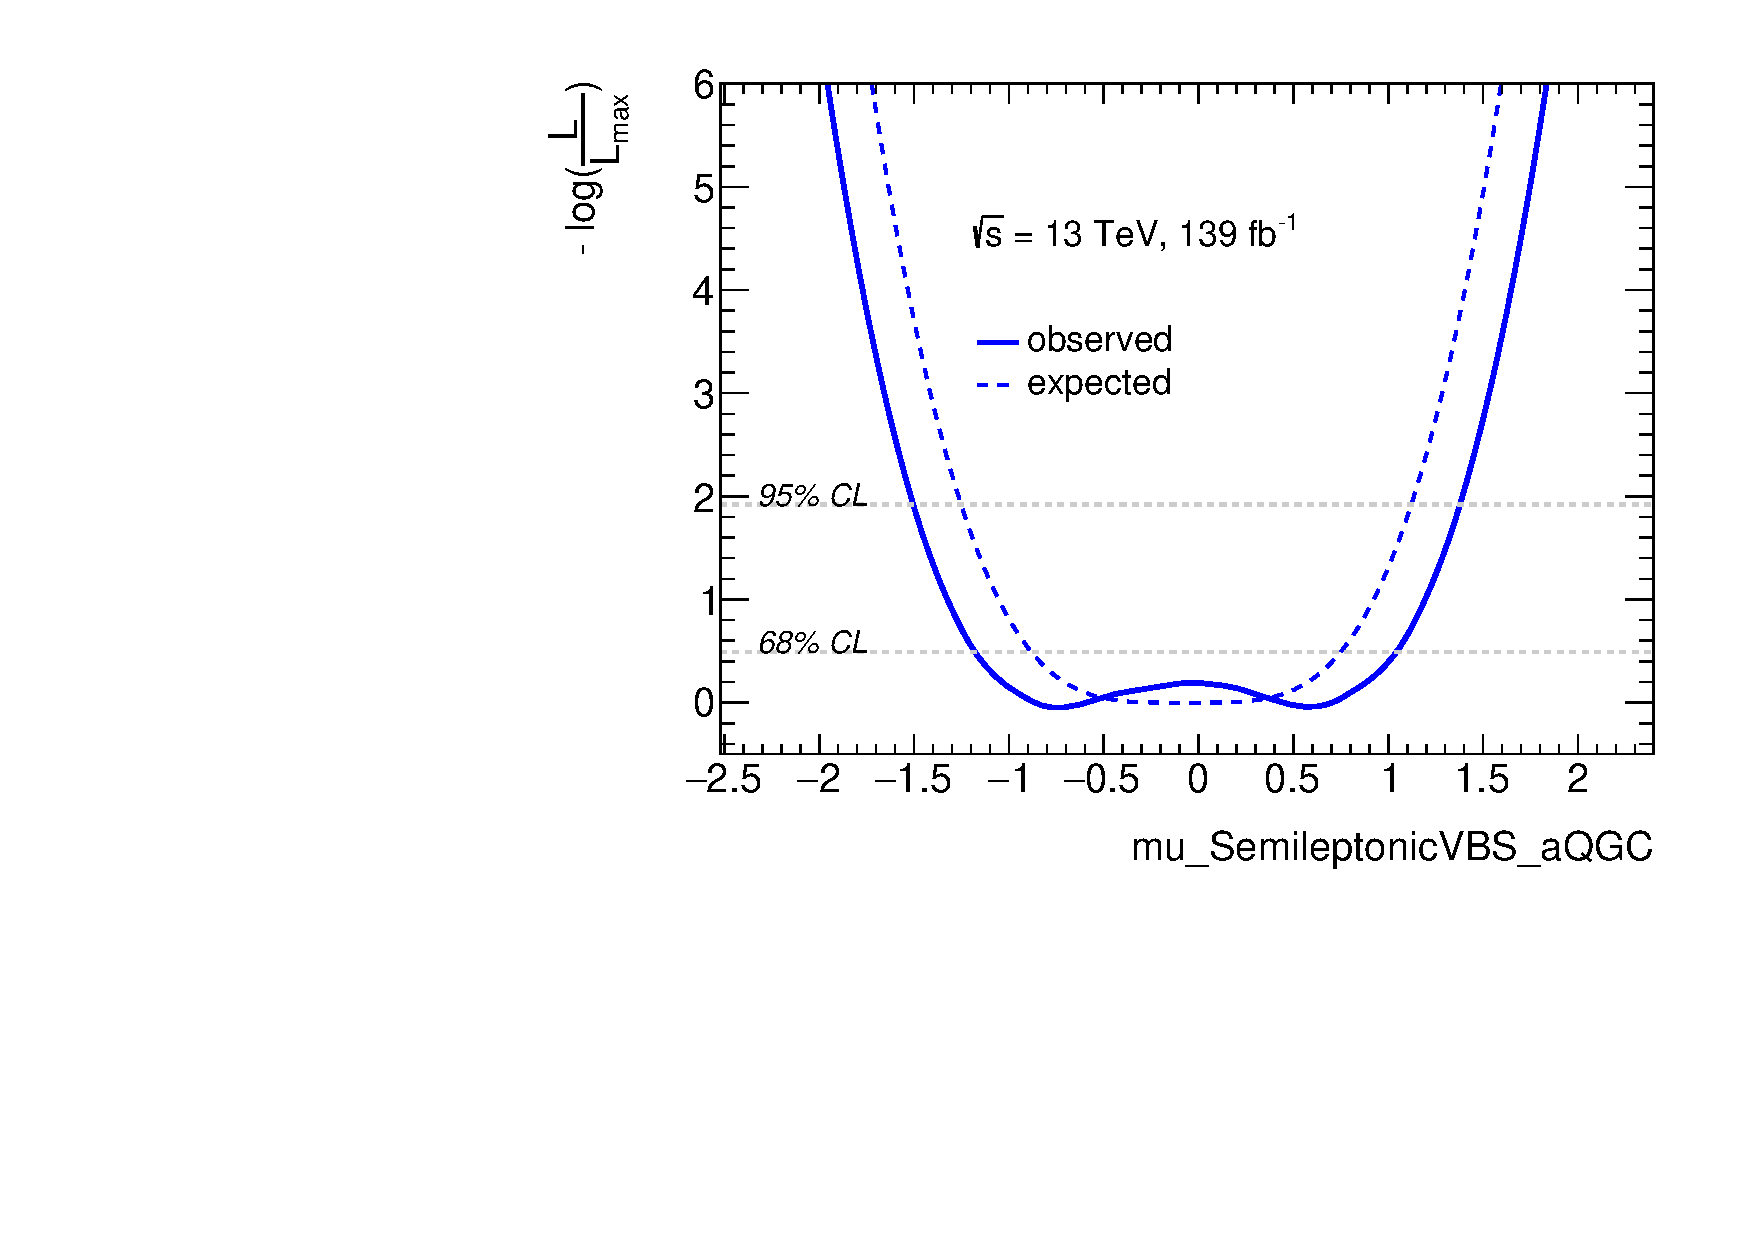
\includegraphics[width=0.32\textwidth]{figures/aQGC/profileFT52000}
    	%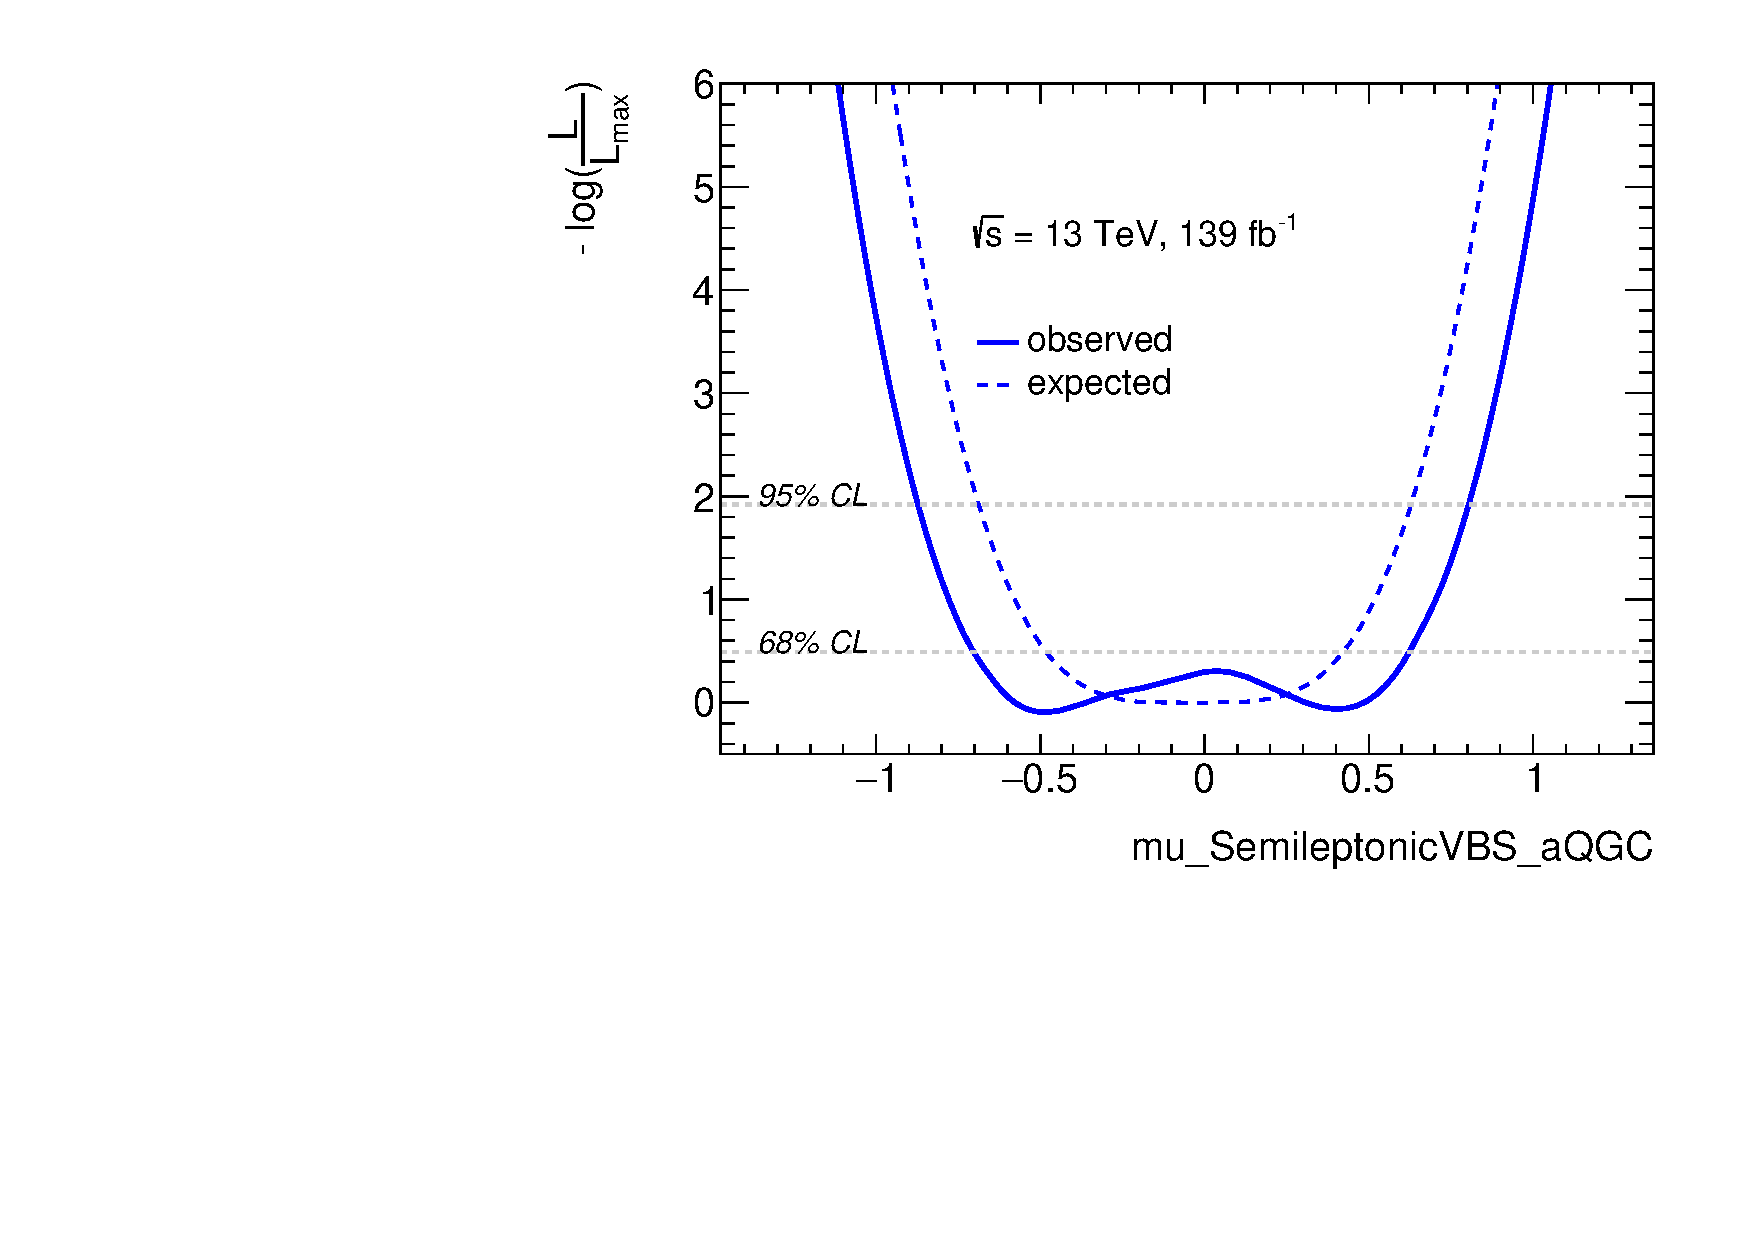
\includegraphics[width=0.38\textwidth]{figures/aQGC/profileFT53000}
        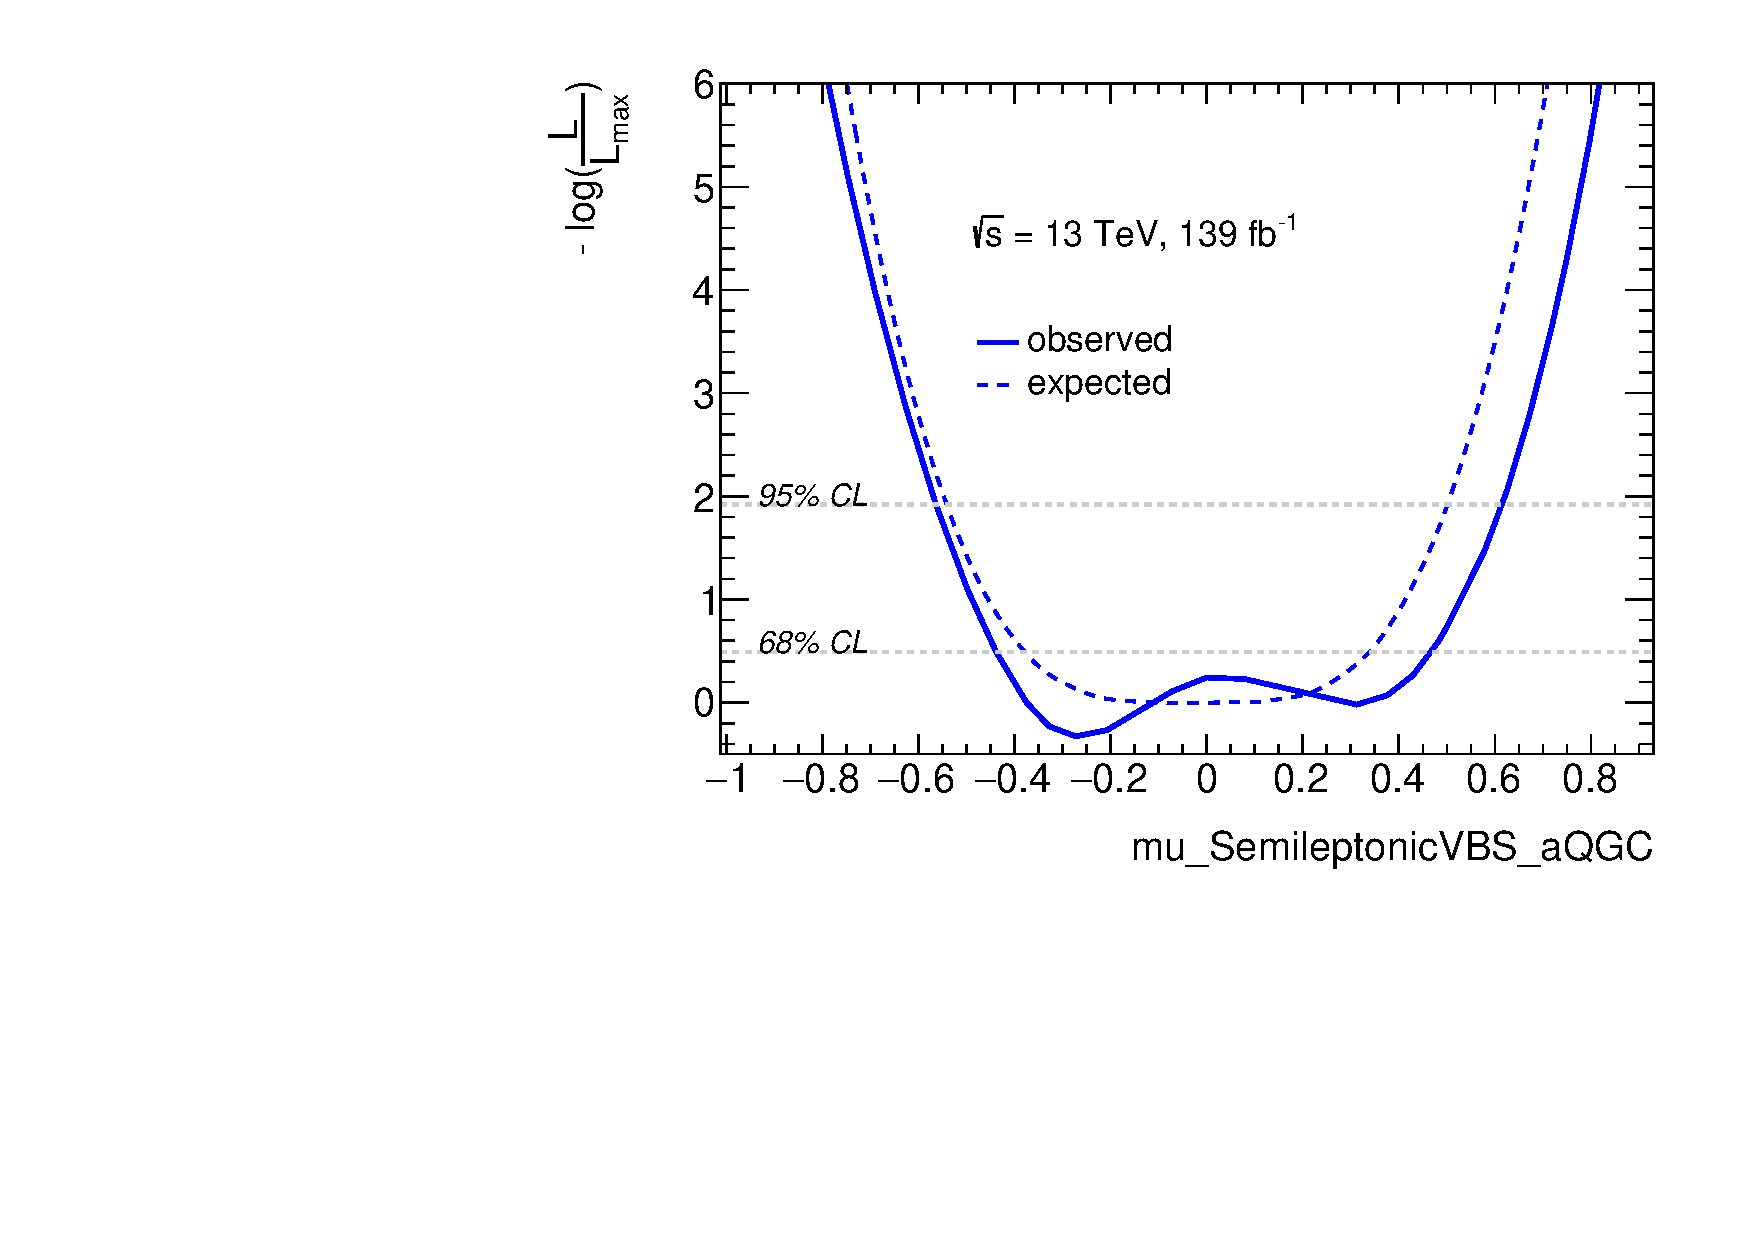
\includegraphics[width=0.32\textwidth]{figures/aQGC/profileFT5inf}
        \caption{The observed log-likelihood curves of FT5 Wilson coefficient where the clipping energy is 1.5~TeV (left), 2.0~TeV (middle), $\infty$ (right).}
        \label{fig:ProfileLL}
\end{figure}
\begin{figure}[ht]
    \centering
    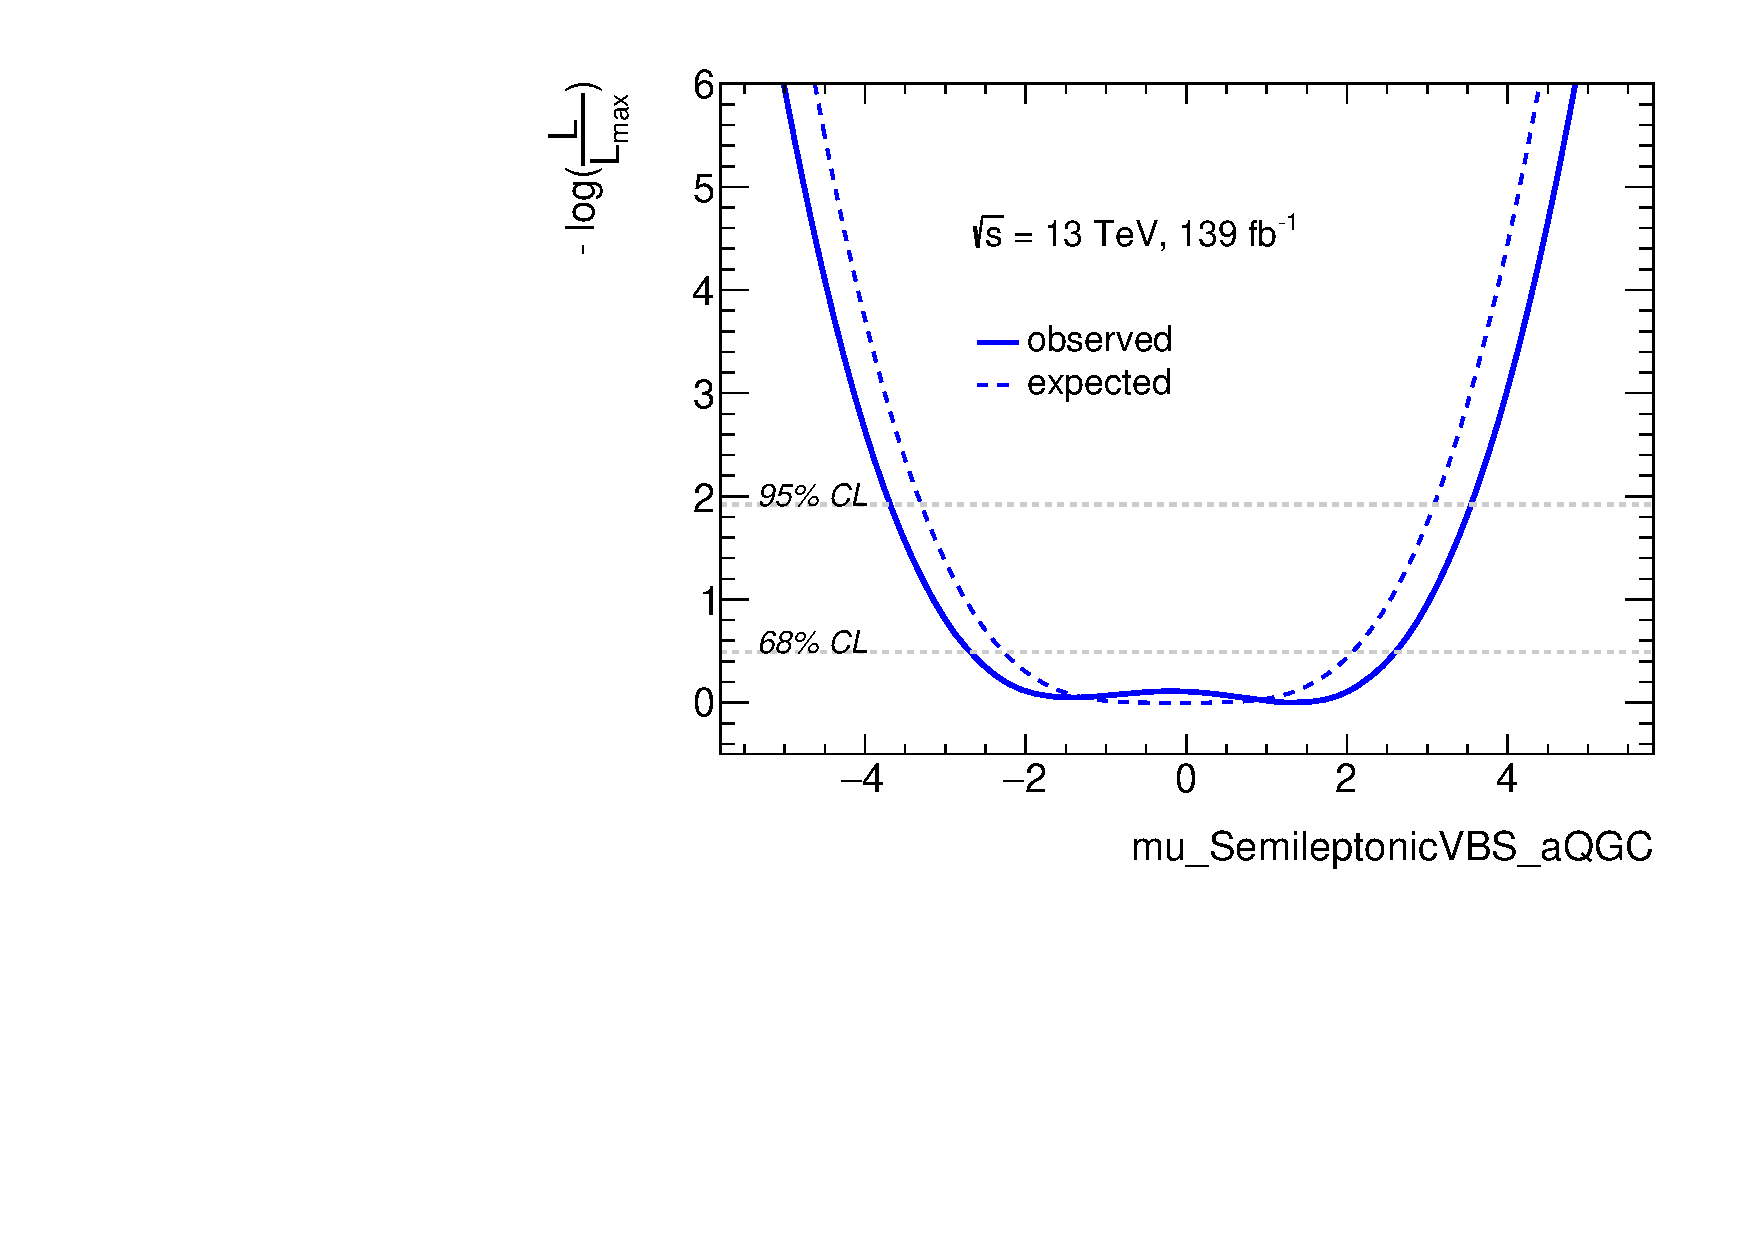
\includegraphics[width=0.32\textwidth]{figures/aQGC/profileFT61500}
    	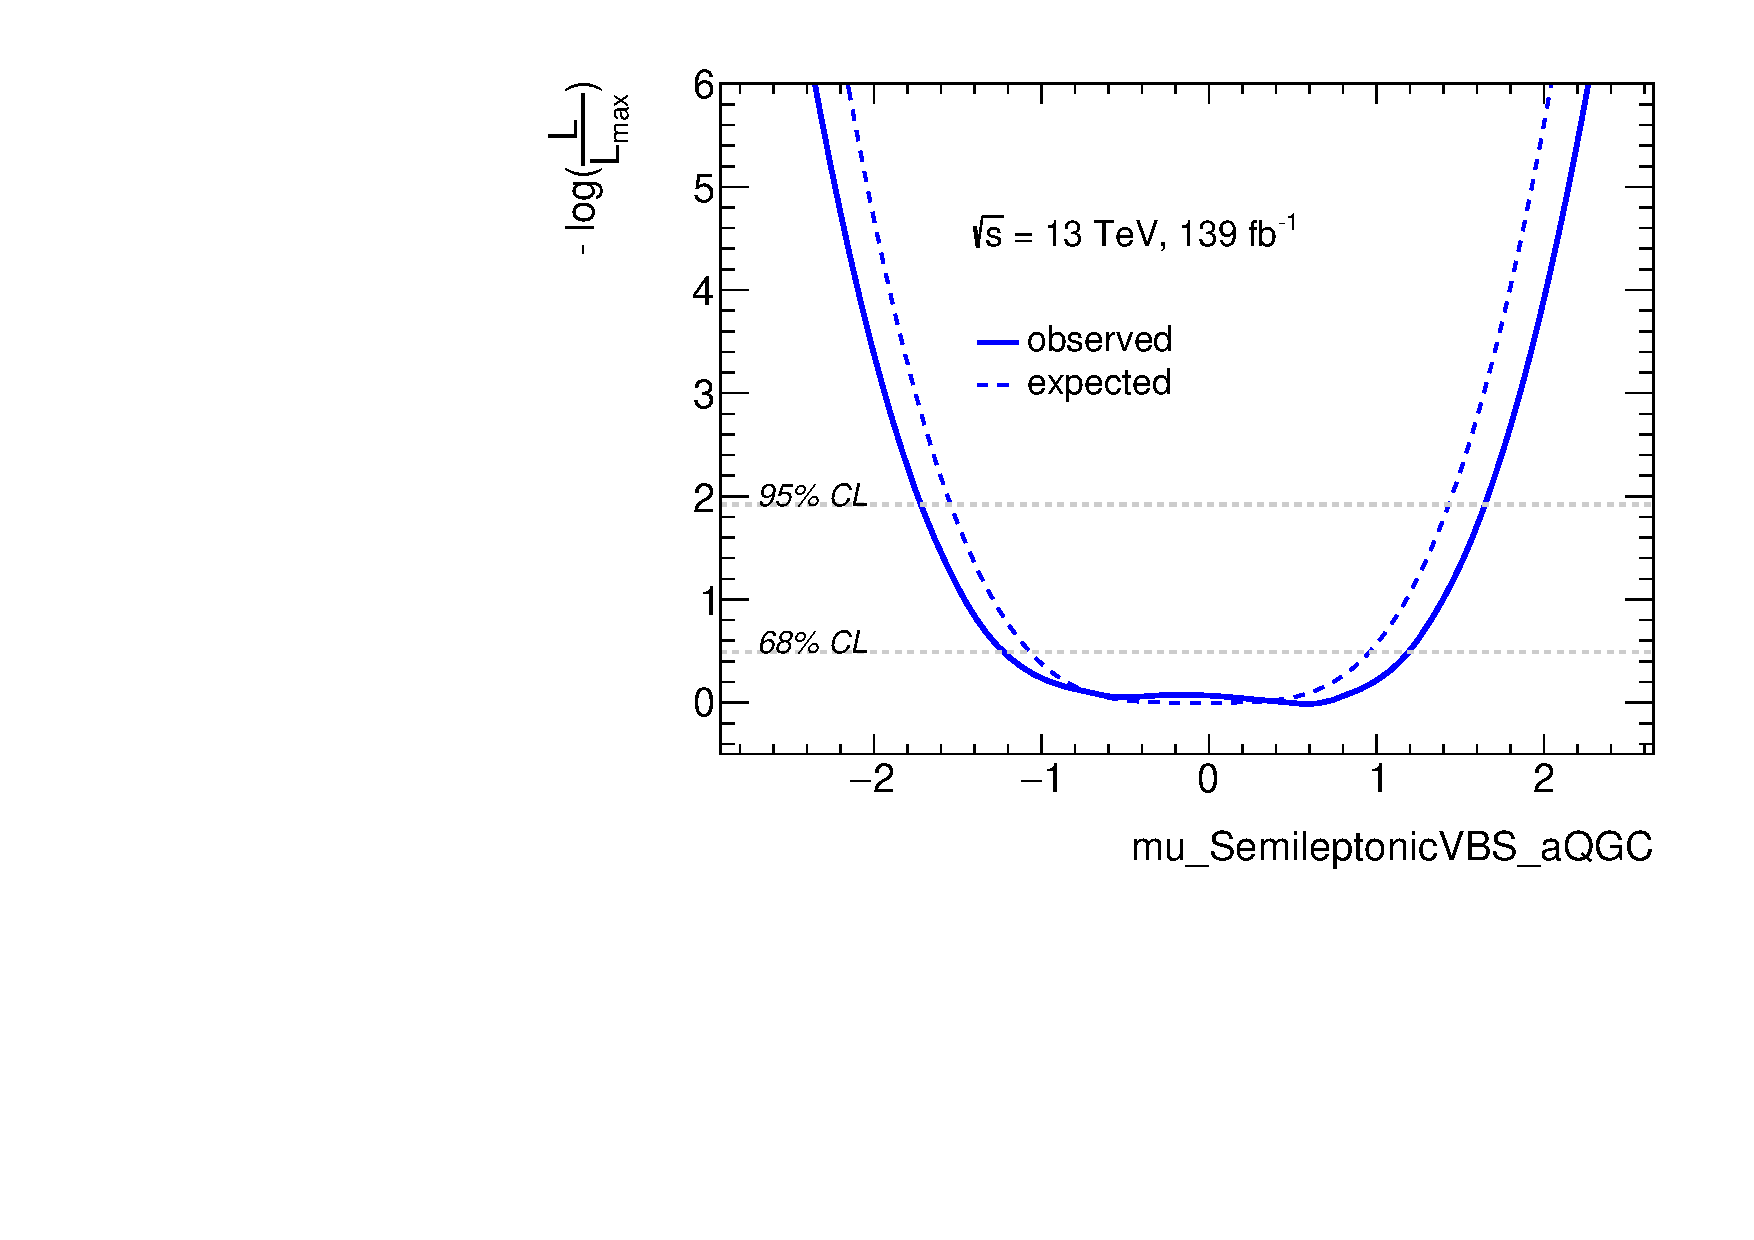
\includegraphics[width=0.32\textwidth]{figures/aQGC/profileFT62000}
    	%\includegraphics[width=0.38\textwidth]{figures/aQGC/profileFT63000}
        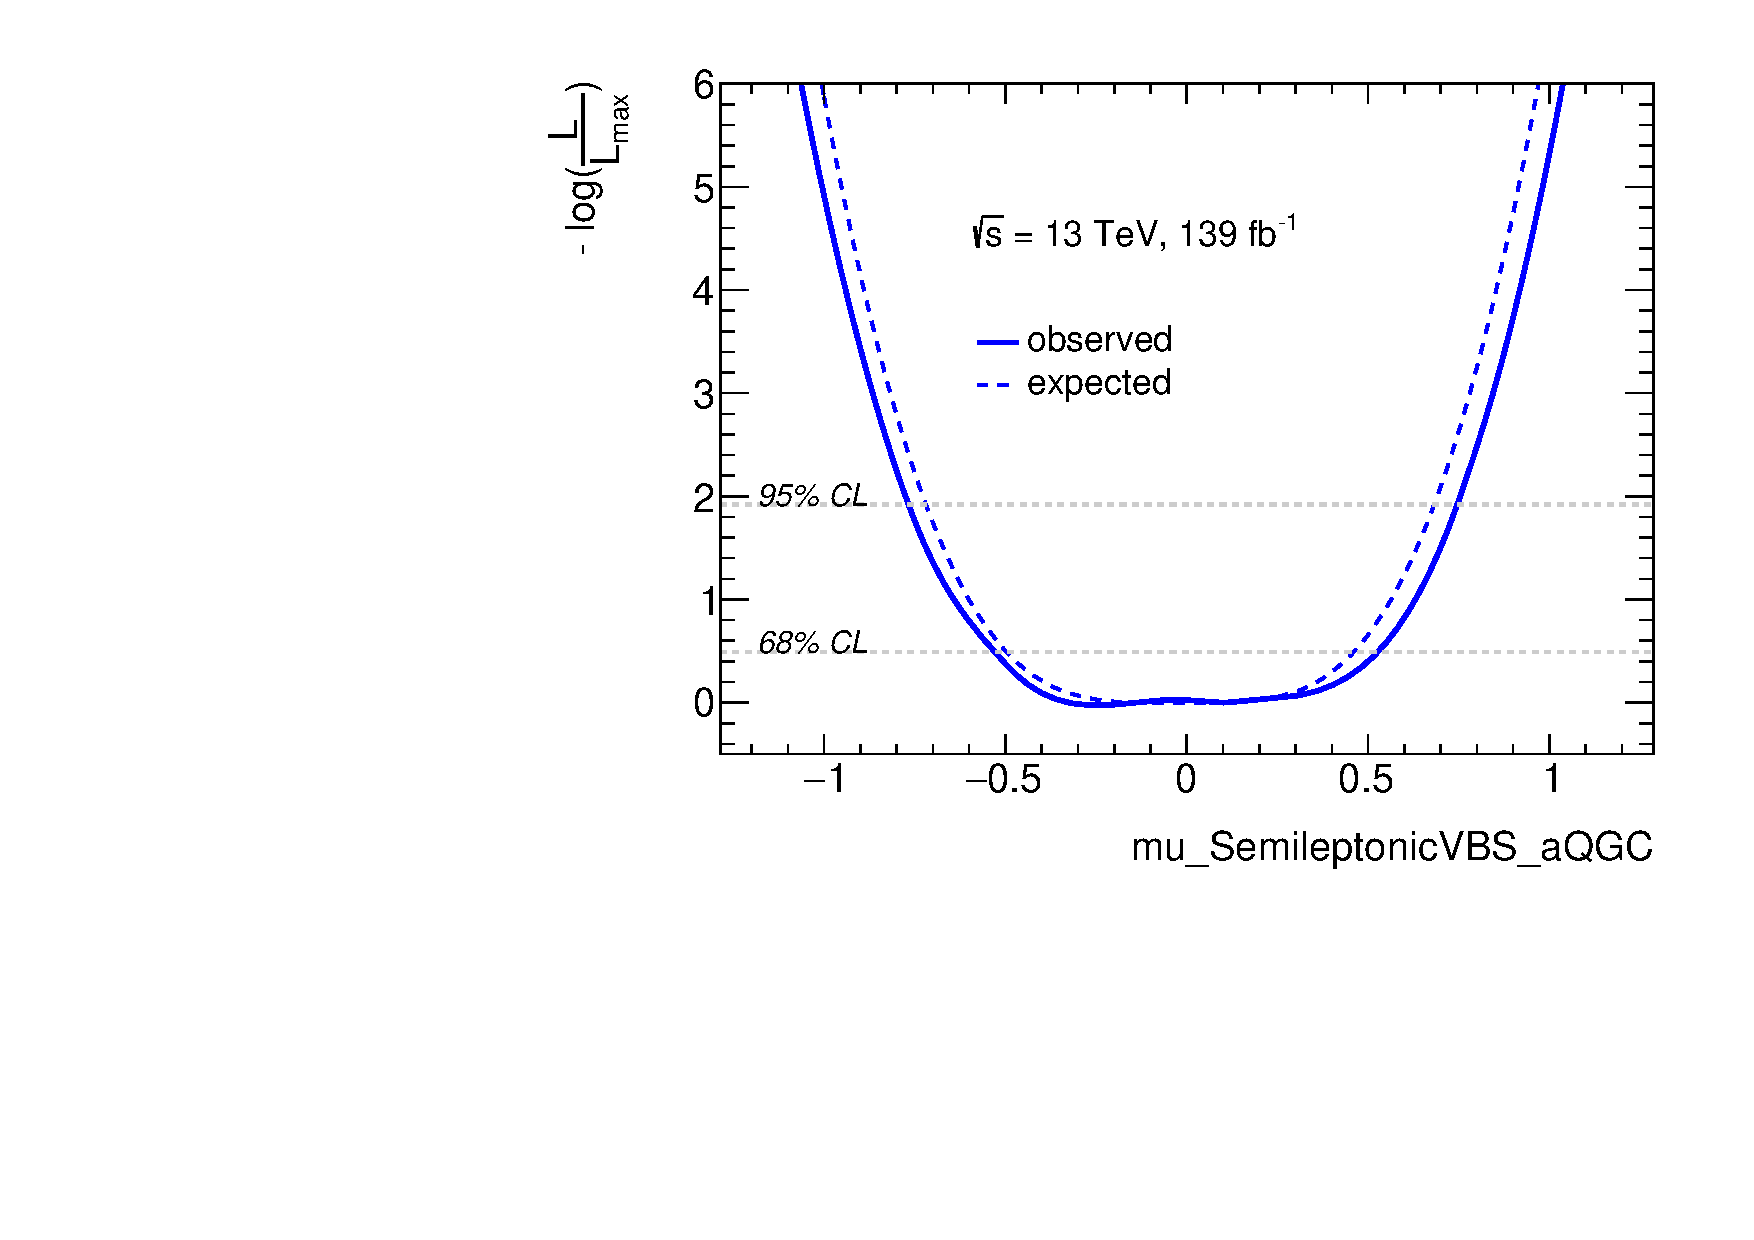
\includegraphics[width=0.32\textwidth]{figures/aQGC/profileFT6inf}
        \caption{The observed log-likelihood curves of FT6 Wilson coefficient where the clipping energy is 1.5~TeV (left), 2.0~TeV (middle), $\infty$ (right).}
        \label{fig:ProfileLL}
\end{figure}
\begin{figure}[ht]
    \centering
    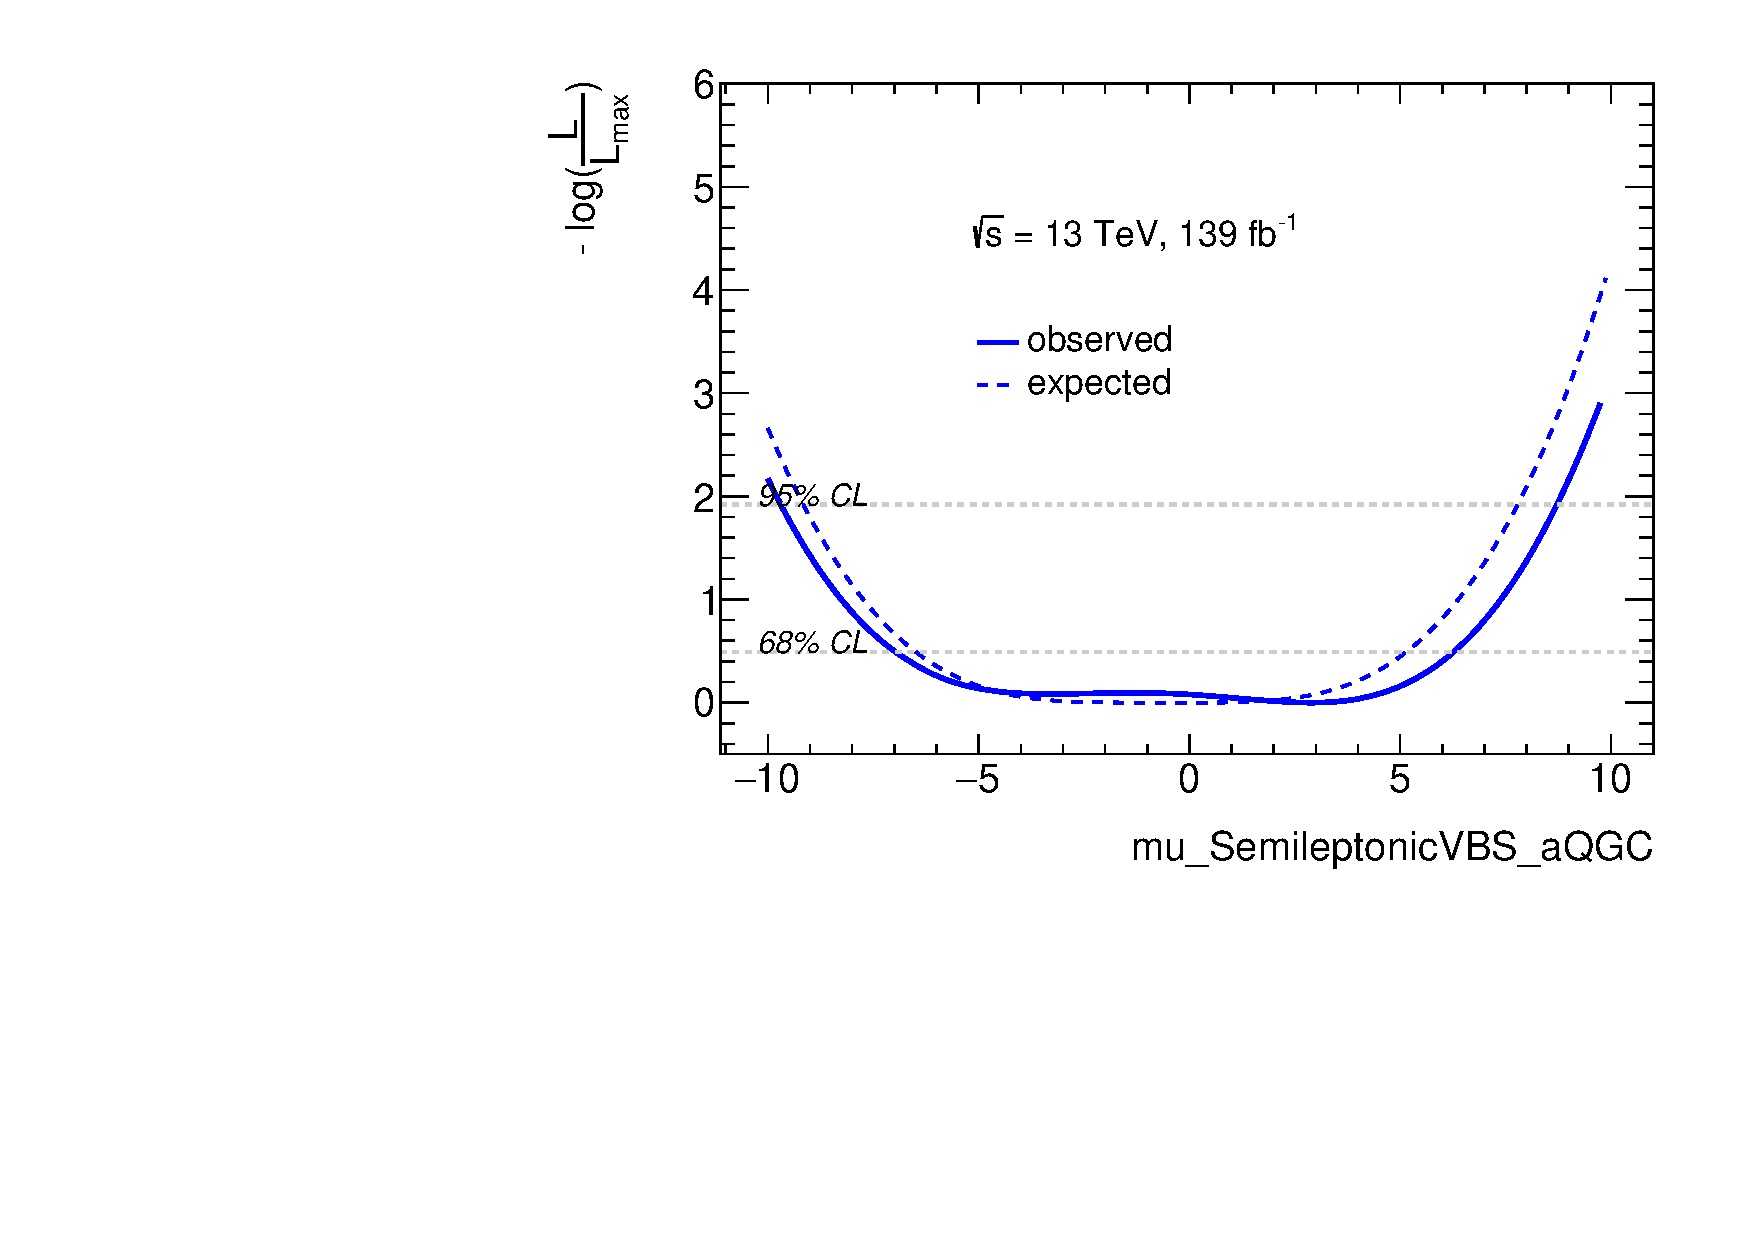
\includegraphics[width=0.32\textwidth]{figures/aQGC/profileFT71500}
    	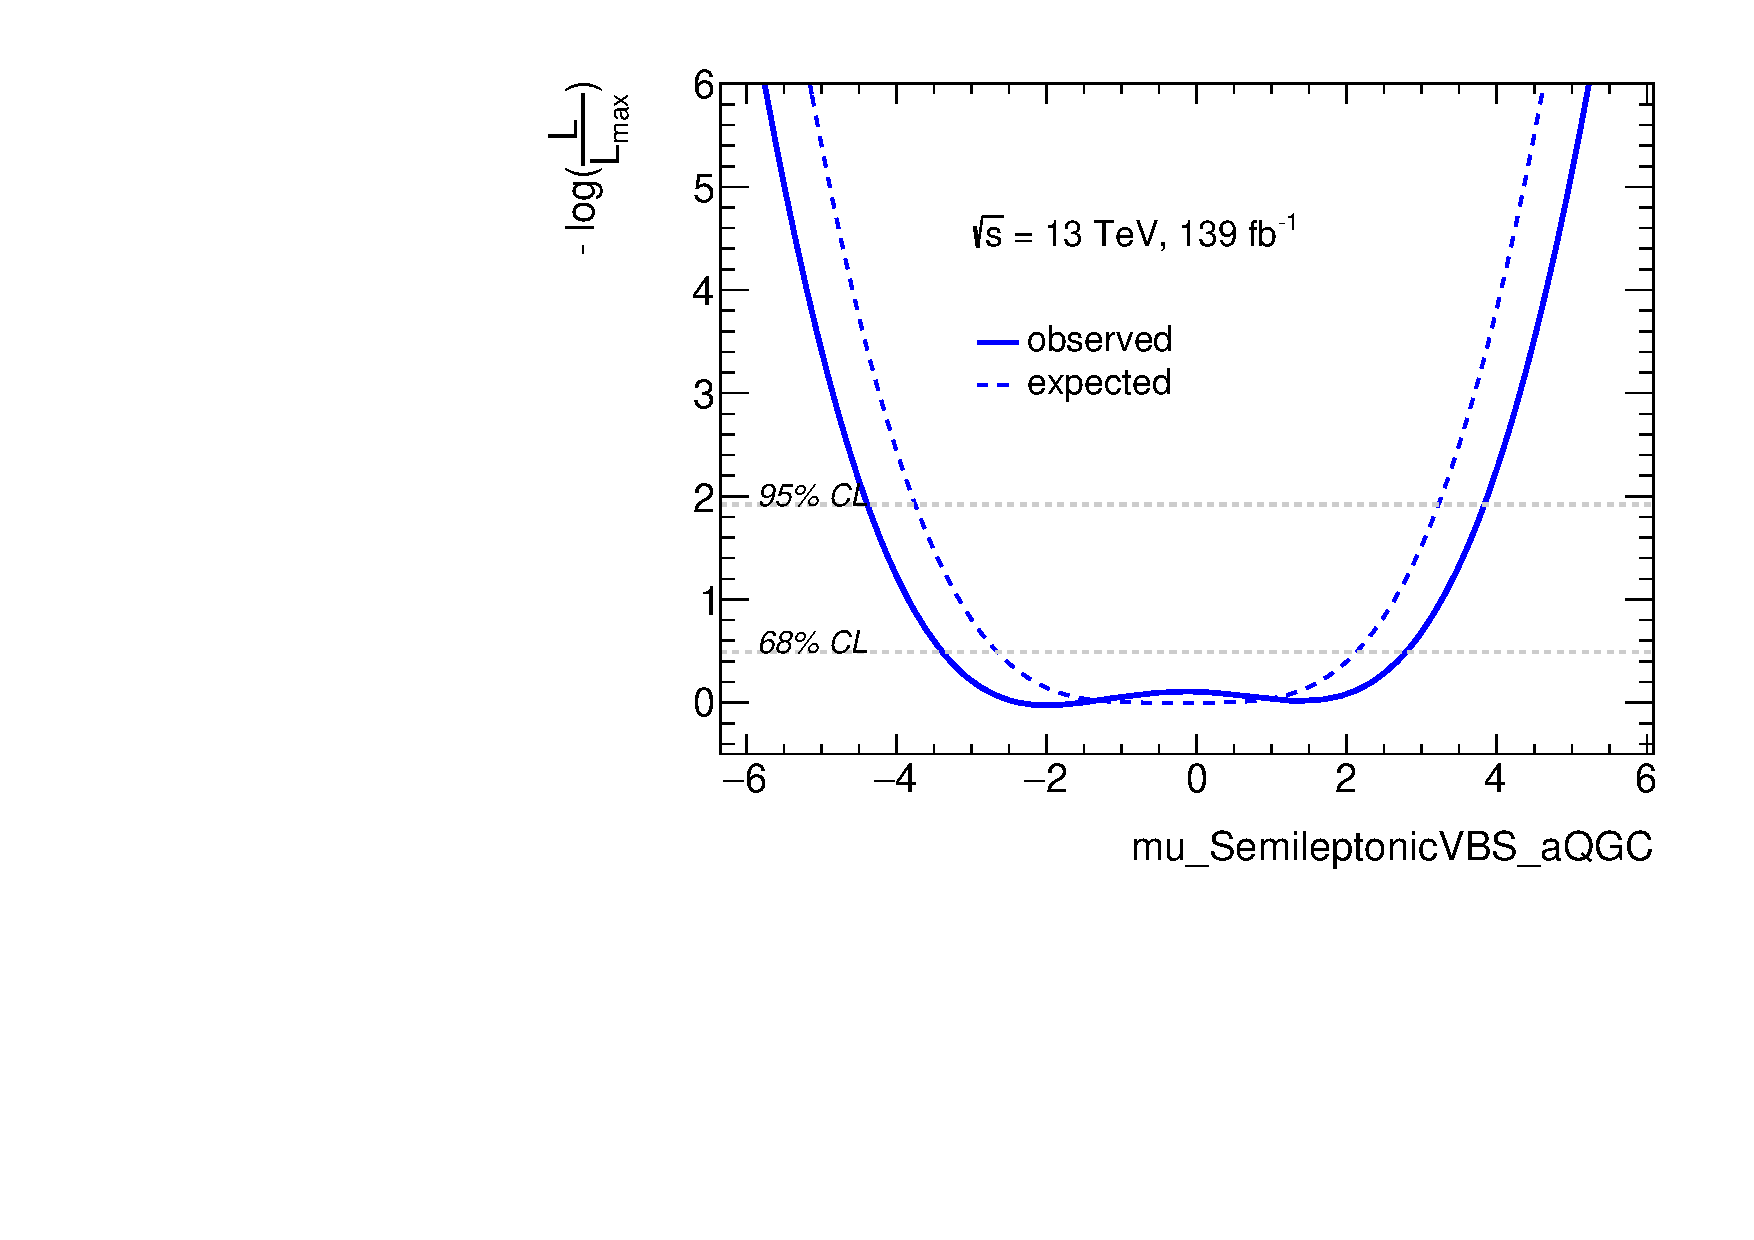
\includegraphics[width=0.32\textwidth]{figures/aQGC/profileFT72000}
    	%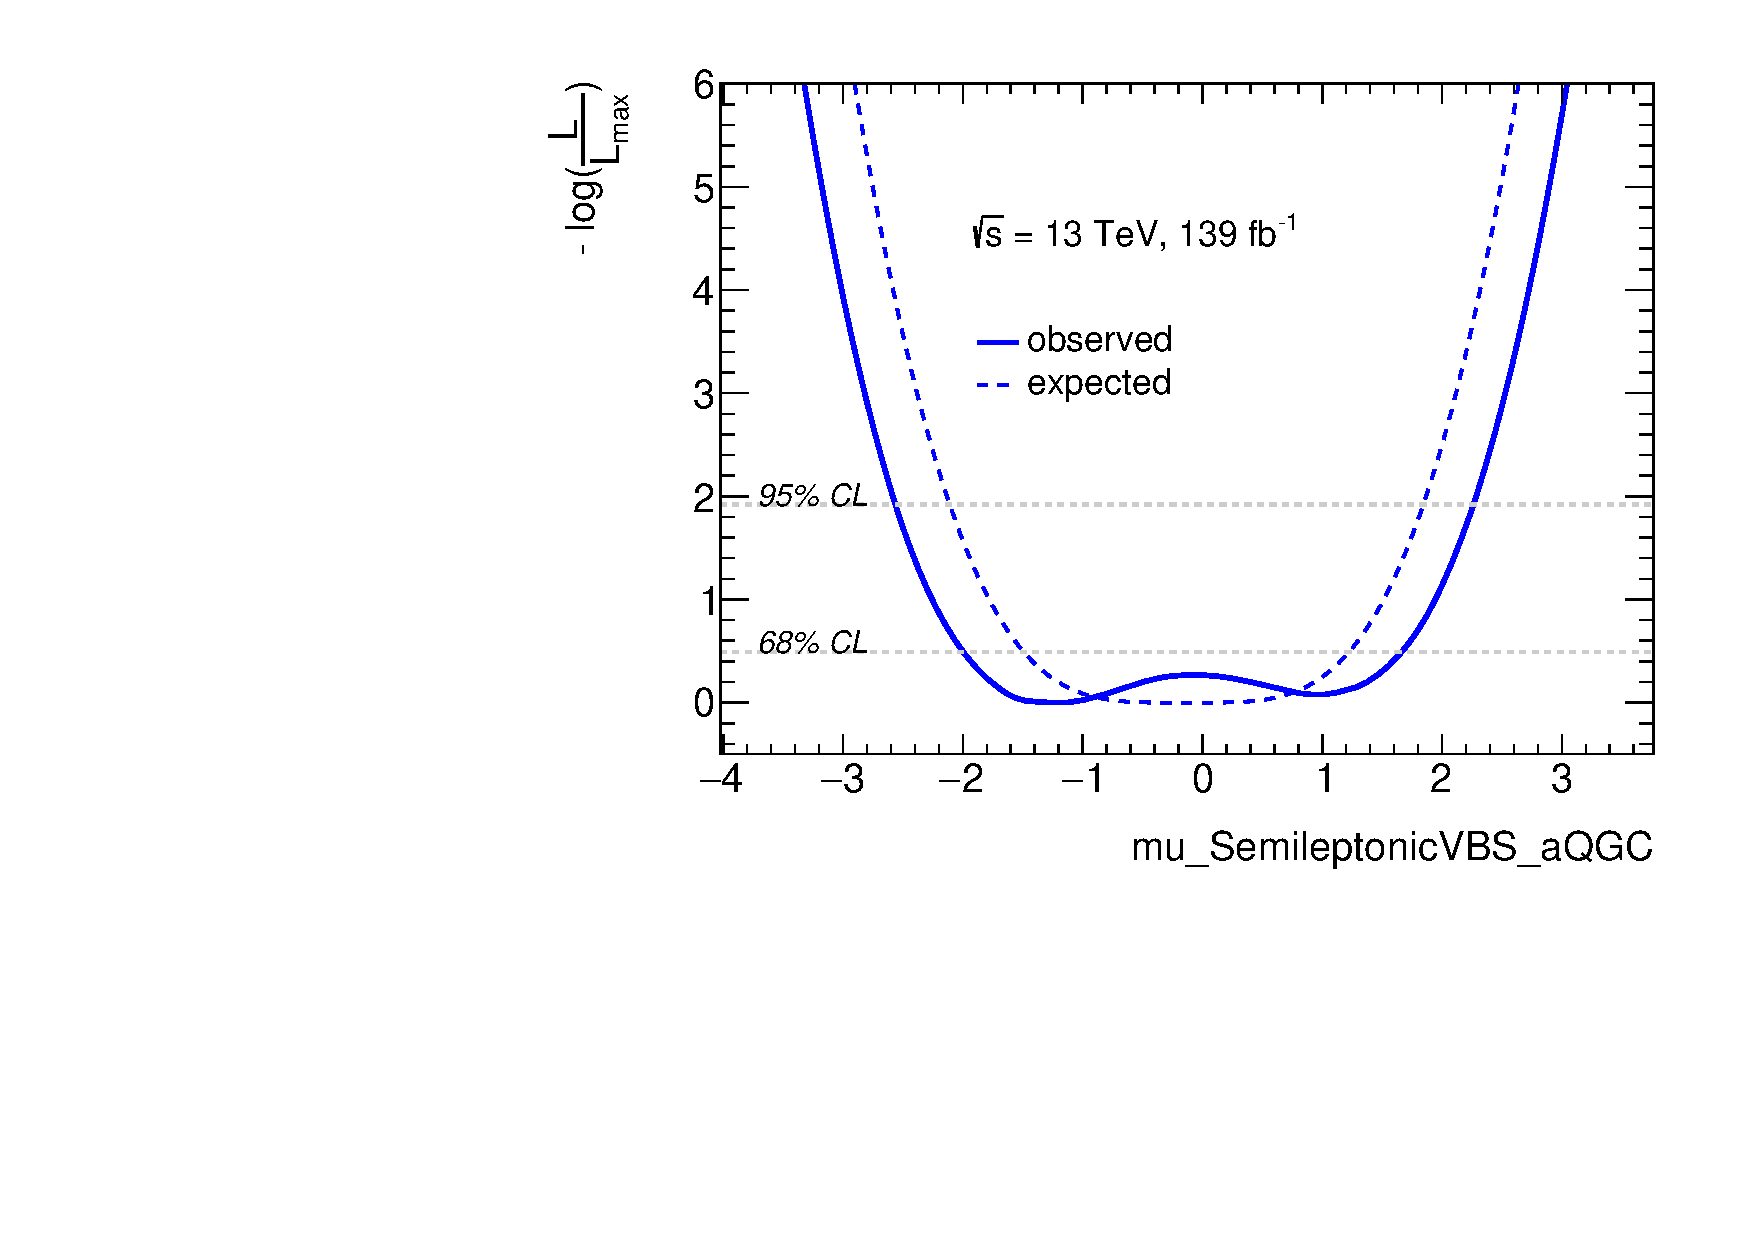
\includegraphics[width=0.38\textwidth]{figures/aQGC/profileFT73000}
        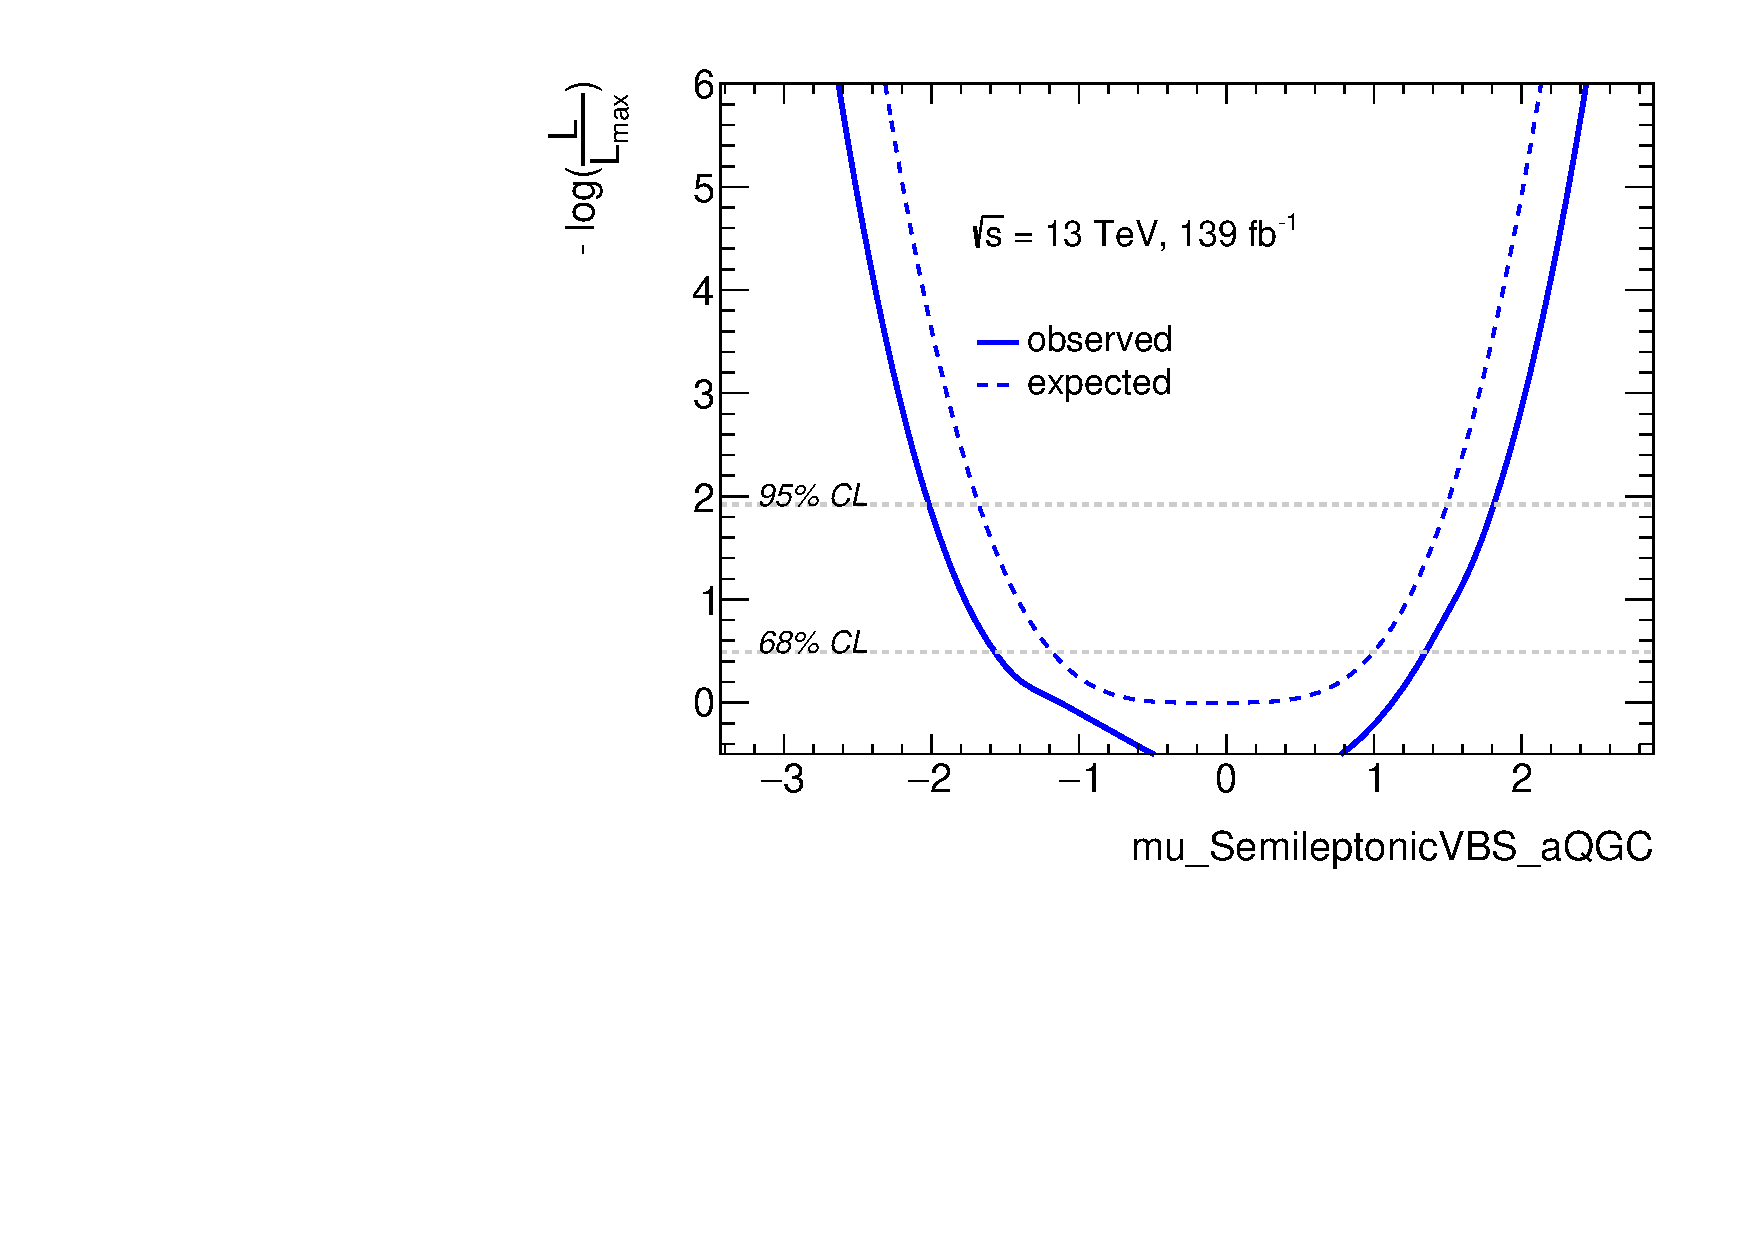
\includegraphics[width=0.32\textwidth]{figures/aQGC/profileFT7inf}
        \caption{The observed log-likelihood curves of FT7 Wilson coefficient where the clipping energy is 1.5~TeV (left), 2.0~TeV (middle), $\infty$ (right).}
        \label{fig:ProfileLL}
\end{figure}
\begin{figure}[ht]
    \centering
    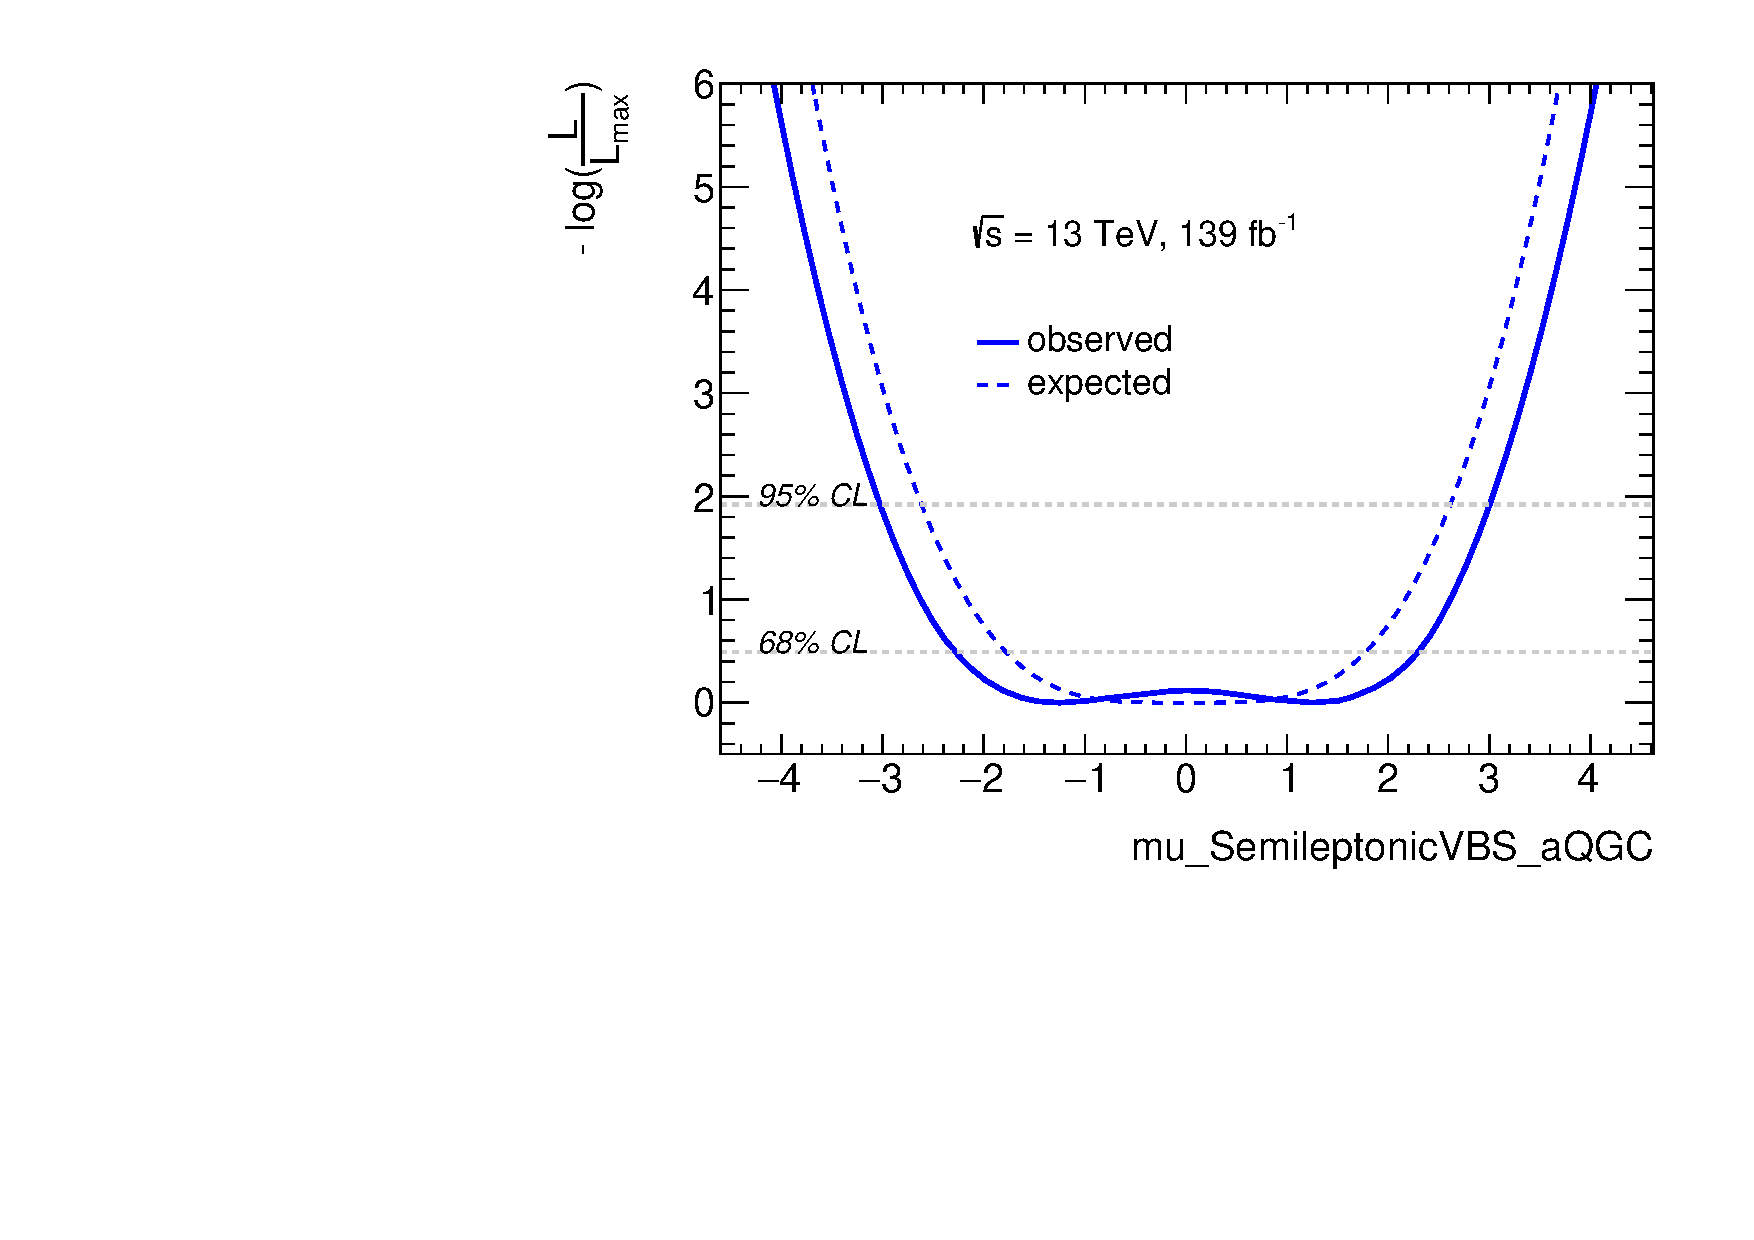
\includegraphics[width=0.32\textwidth]{figures/aQGC/profileFT81500}
    	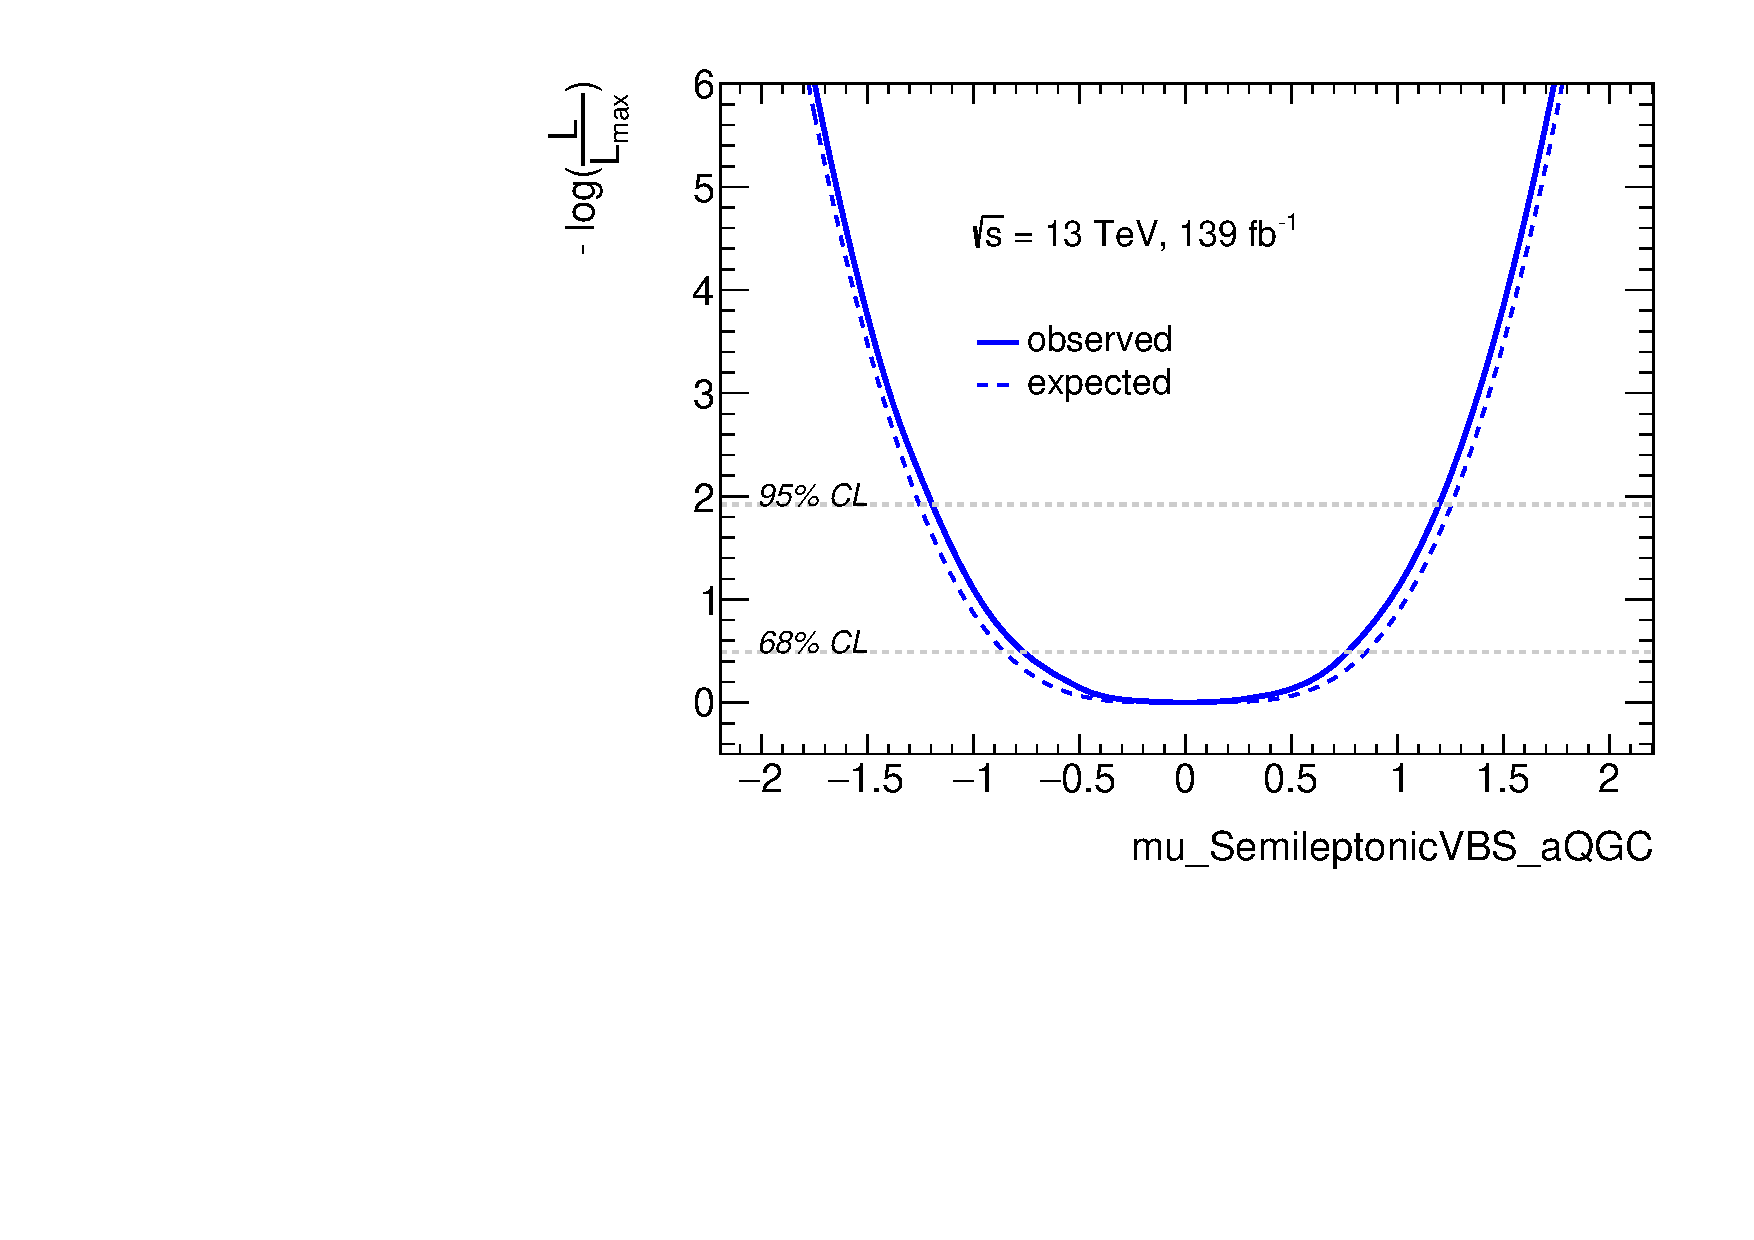
\includegraphics[width=0.32\textwidth]{figures/aQGC/profileFT82000}
    	%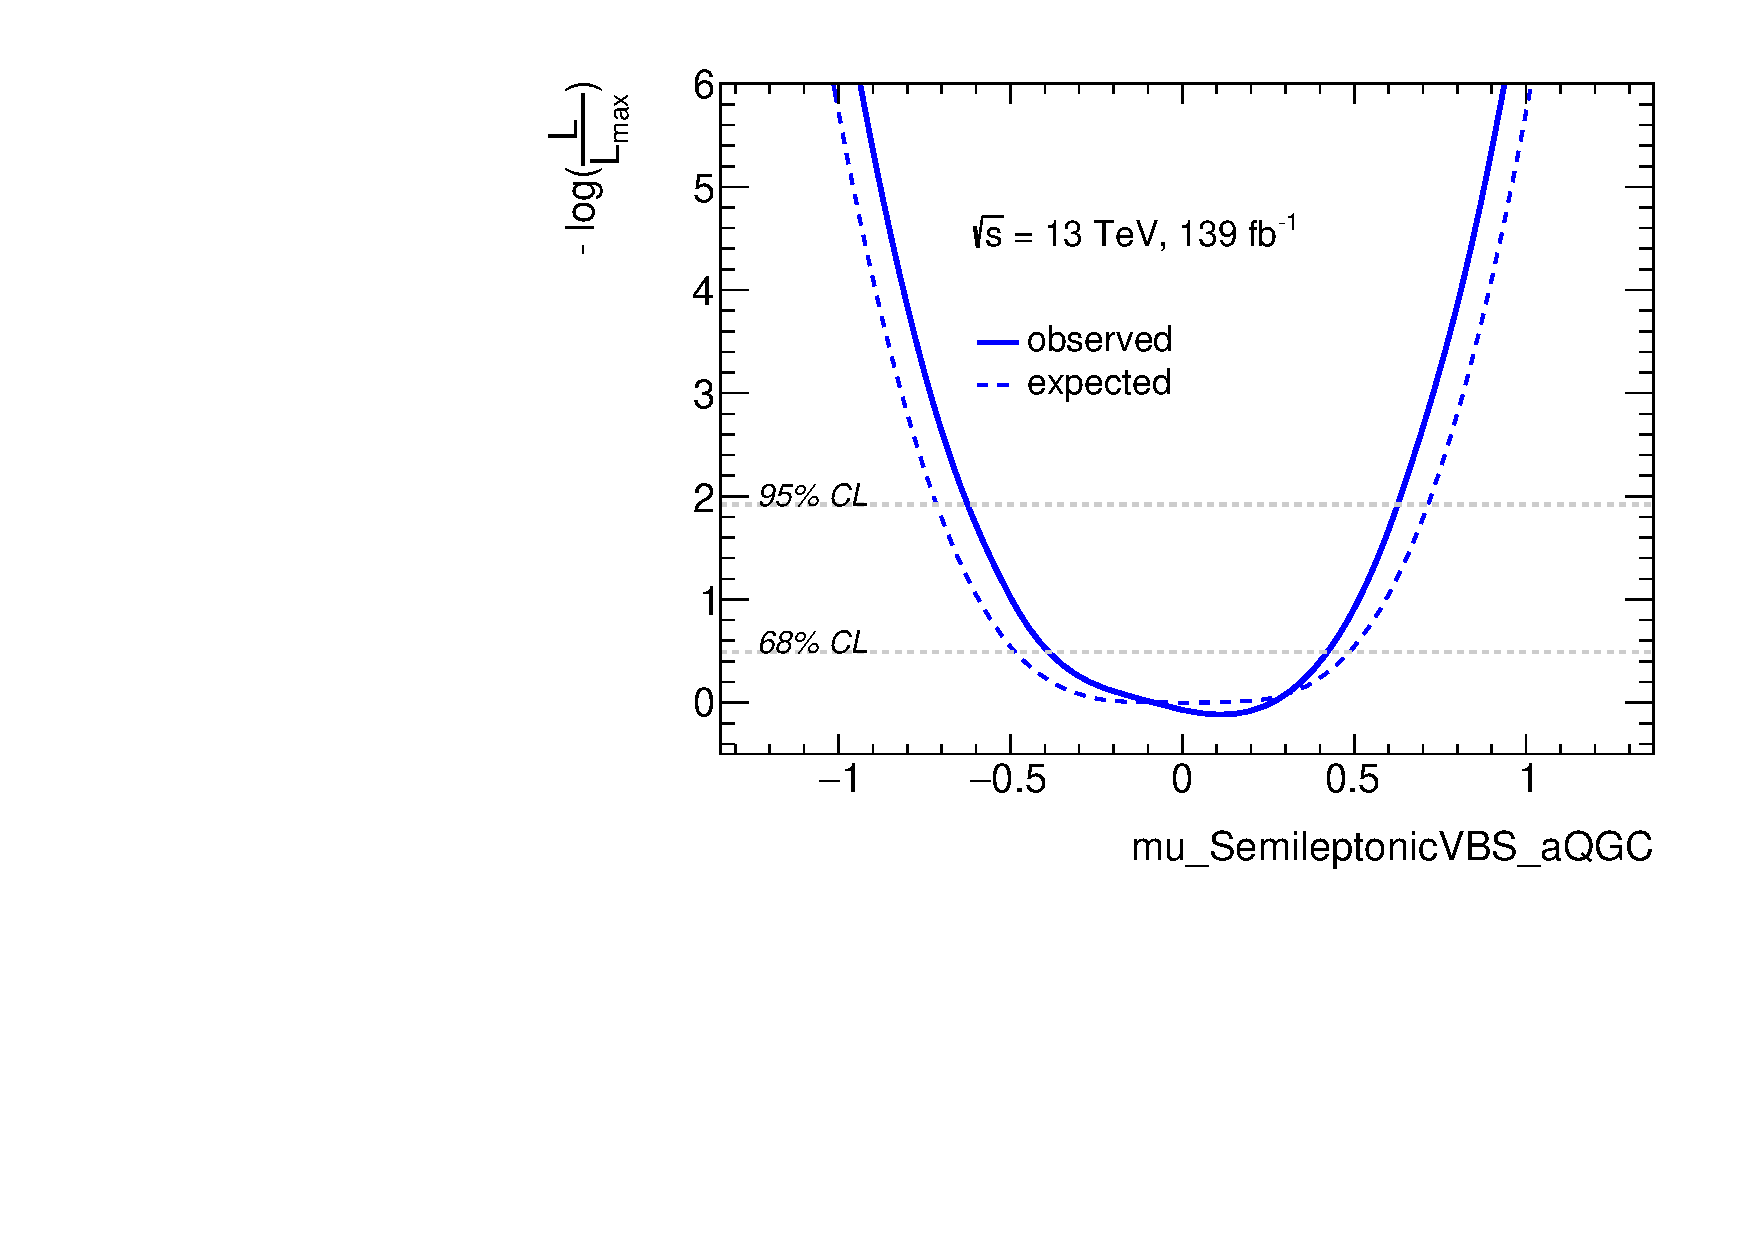
\includegraphics[width=0.38\textwidth]{figures/aQGC/profileFT83000}
        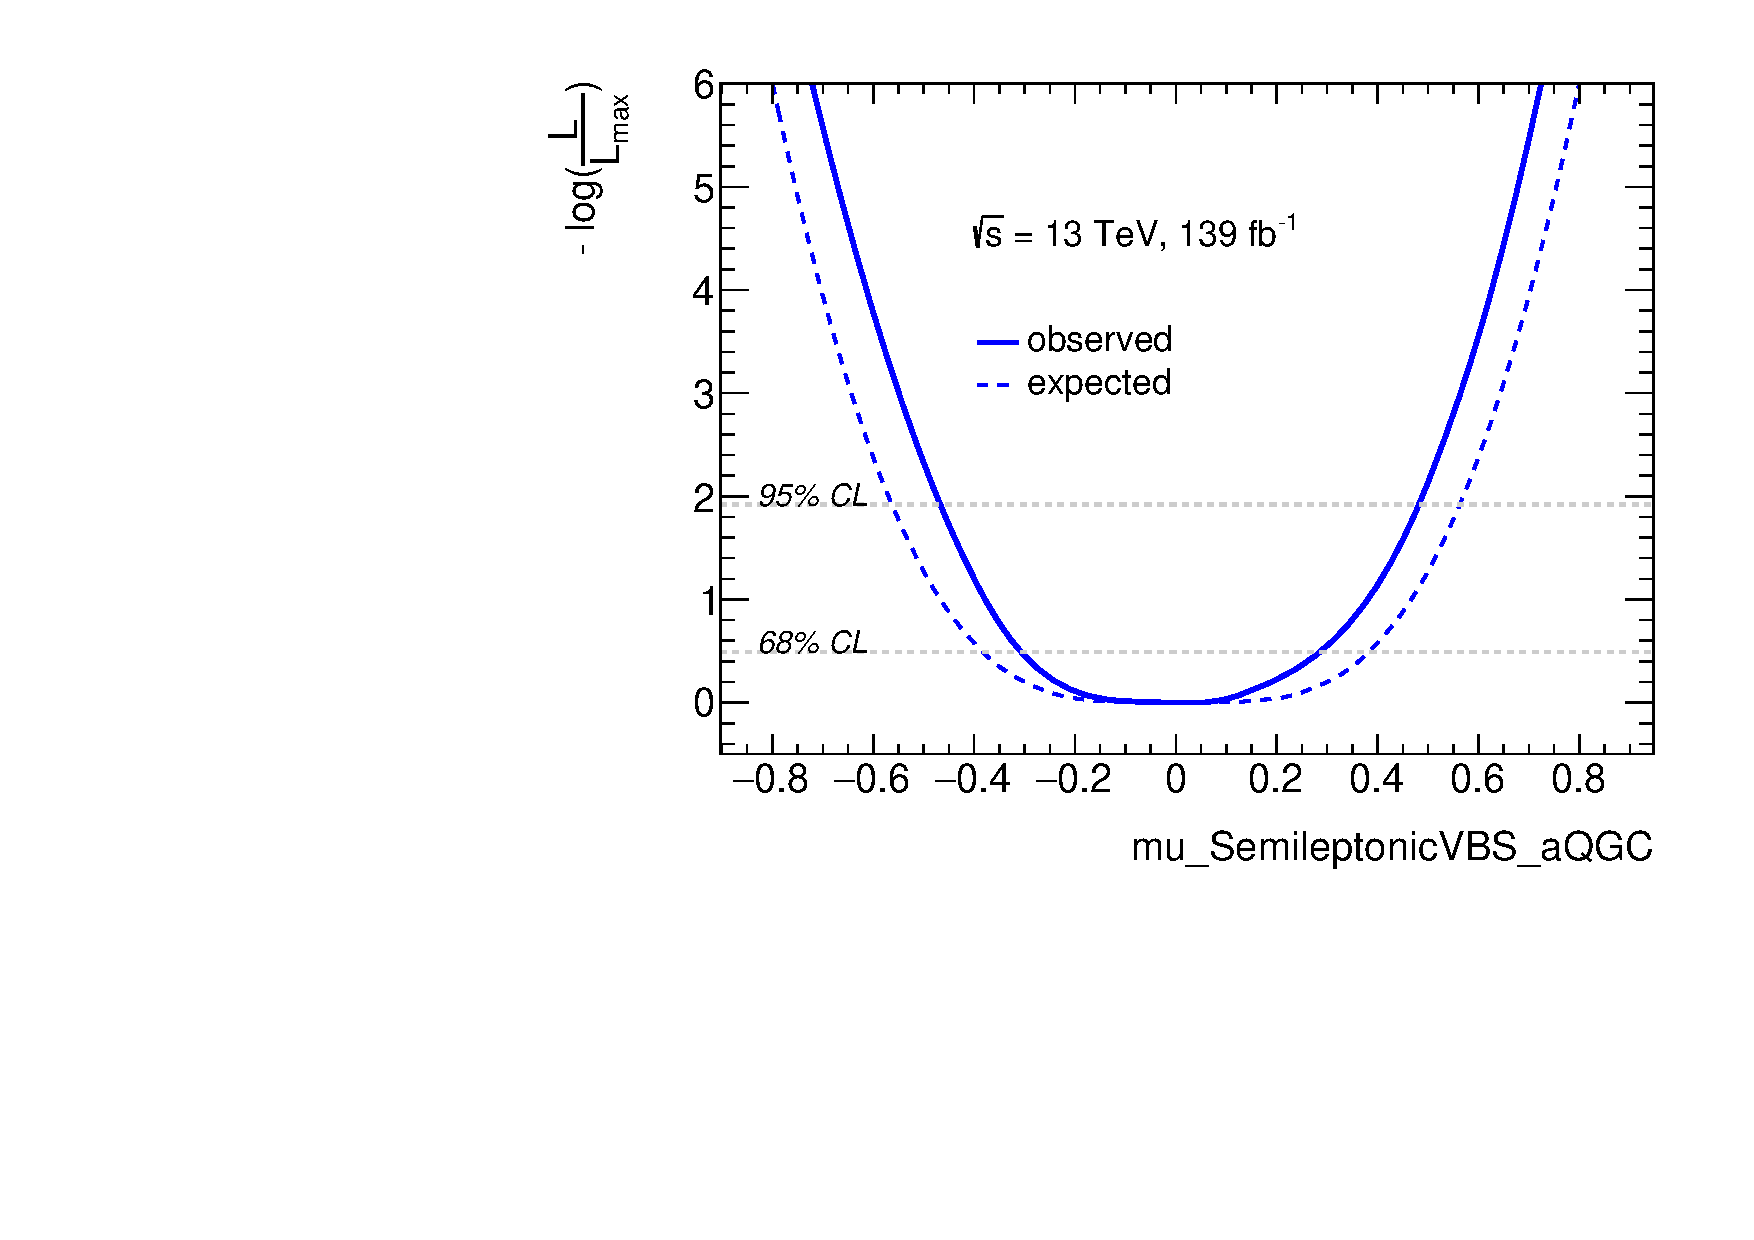
\includegraphics[width=0.32\textwidth]{figures/aQGC/profileFT8inf}
        \caption{The observed log-likelihood curves of FT8 Wilson coefficient where the clipping energy is 1.5~TeV (left), 2.0~TeV (middle), $\infty$ (right).}
        \label{fig:ProfileLL}
\end{figure}

%FS
\begin{figure}[ht]
    \centering
    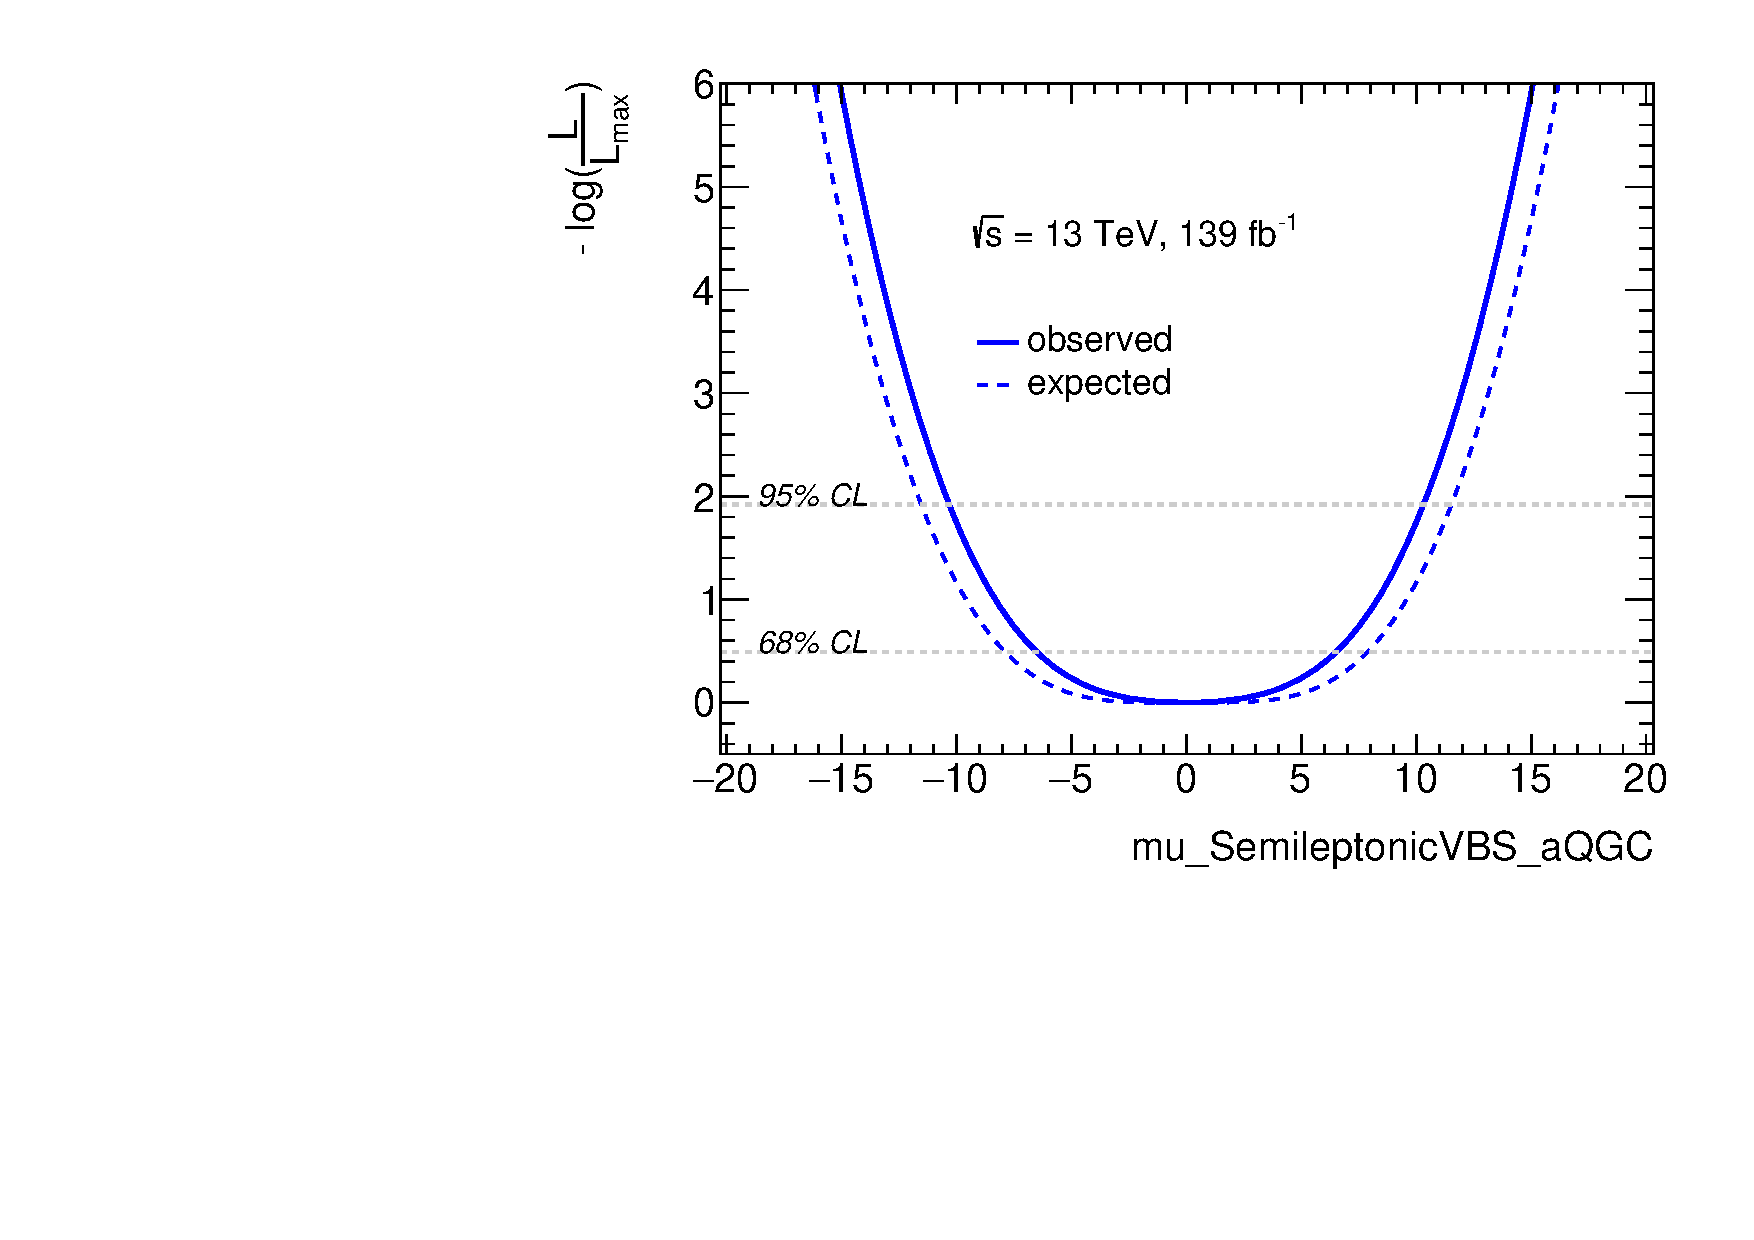
\includegraphics[width=0.32\textwidth]{figures/aQGC/profileFS021500}
    	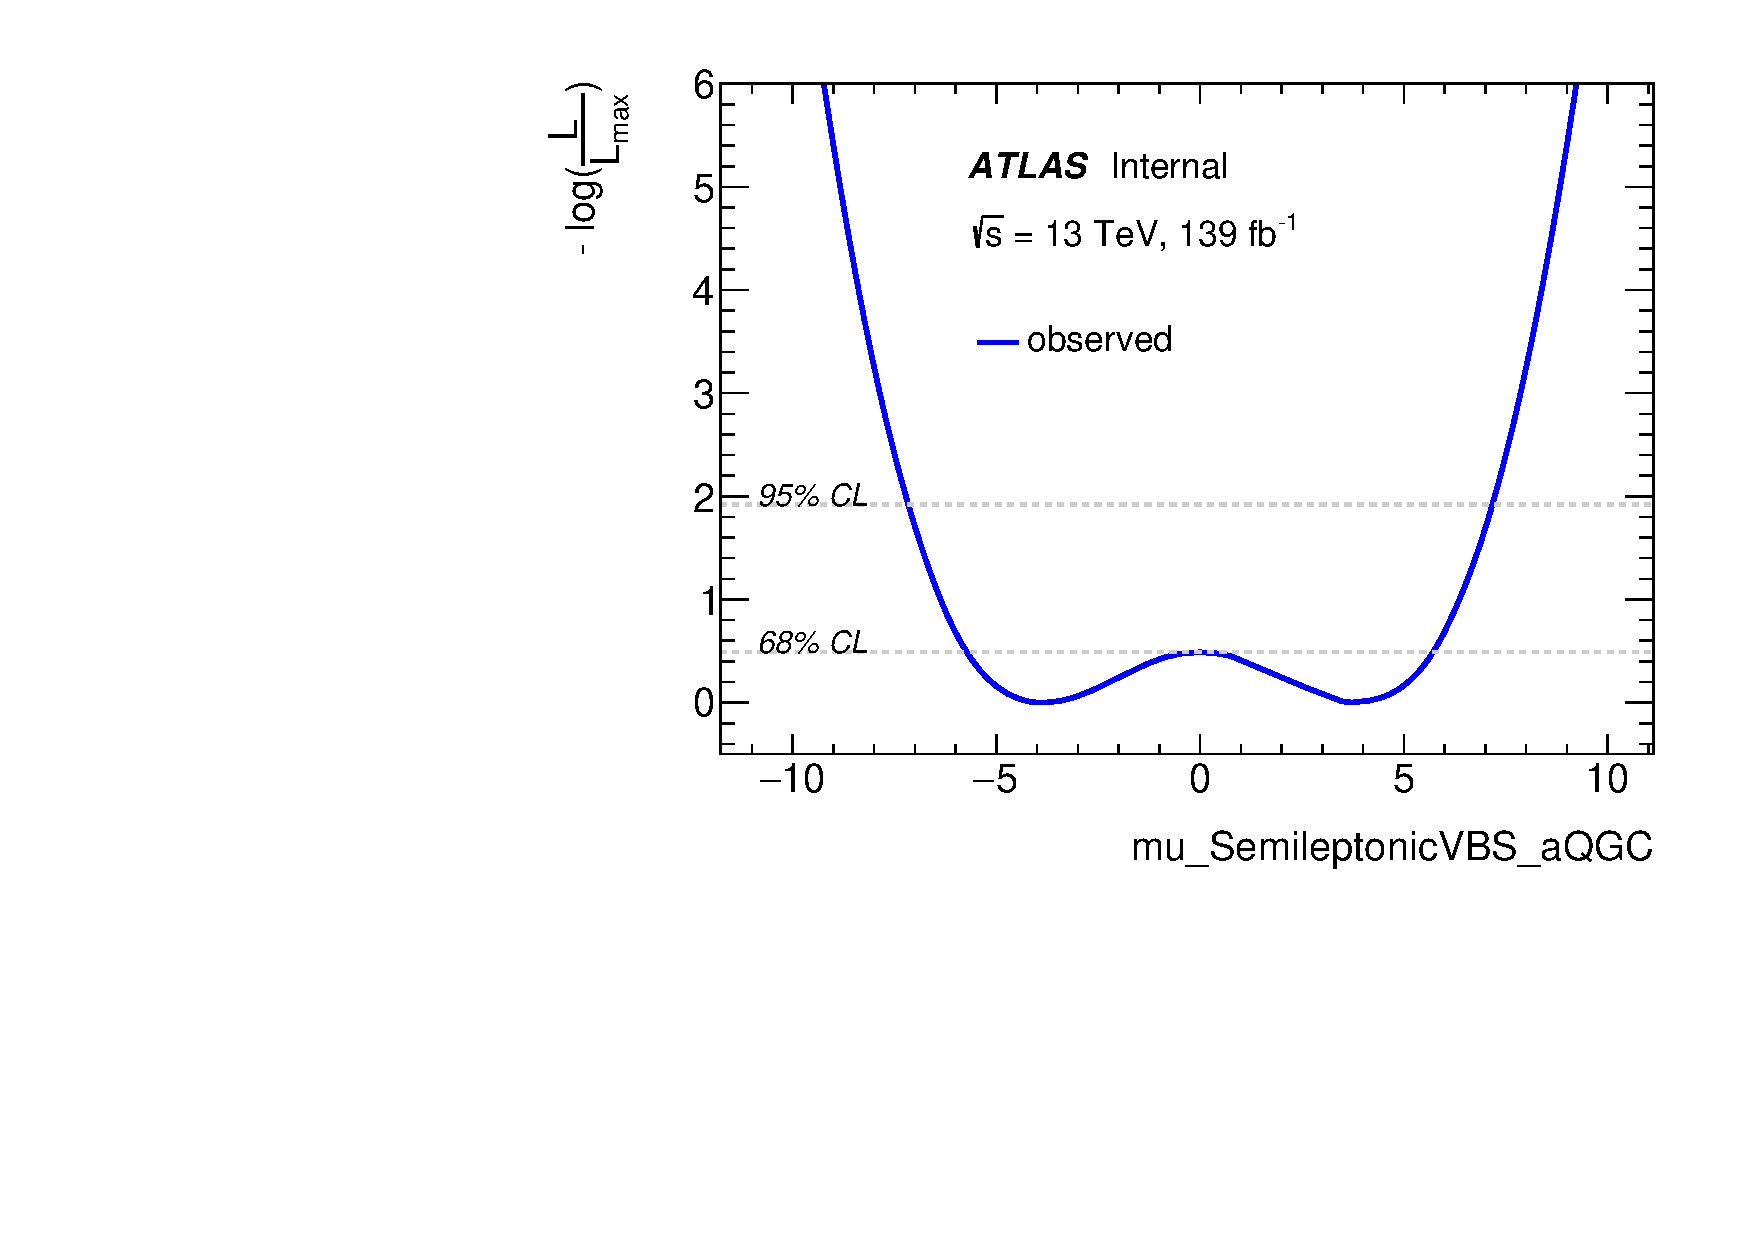
\includegraphics[width=0.32\textwidth]{figures/aQGC/profileFS022000}
    	%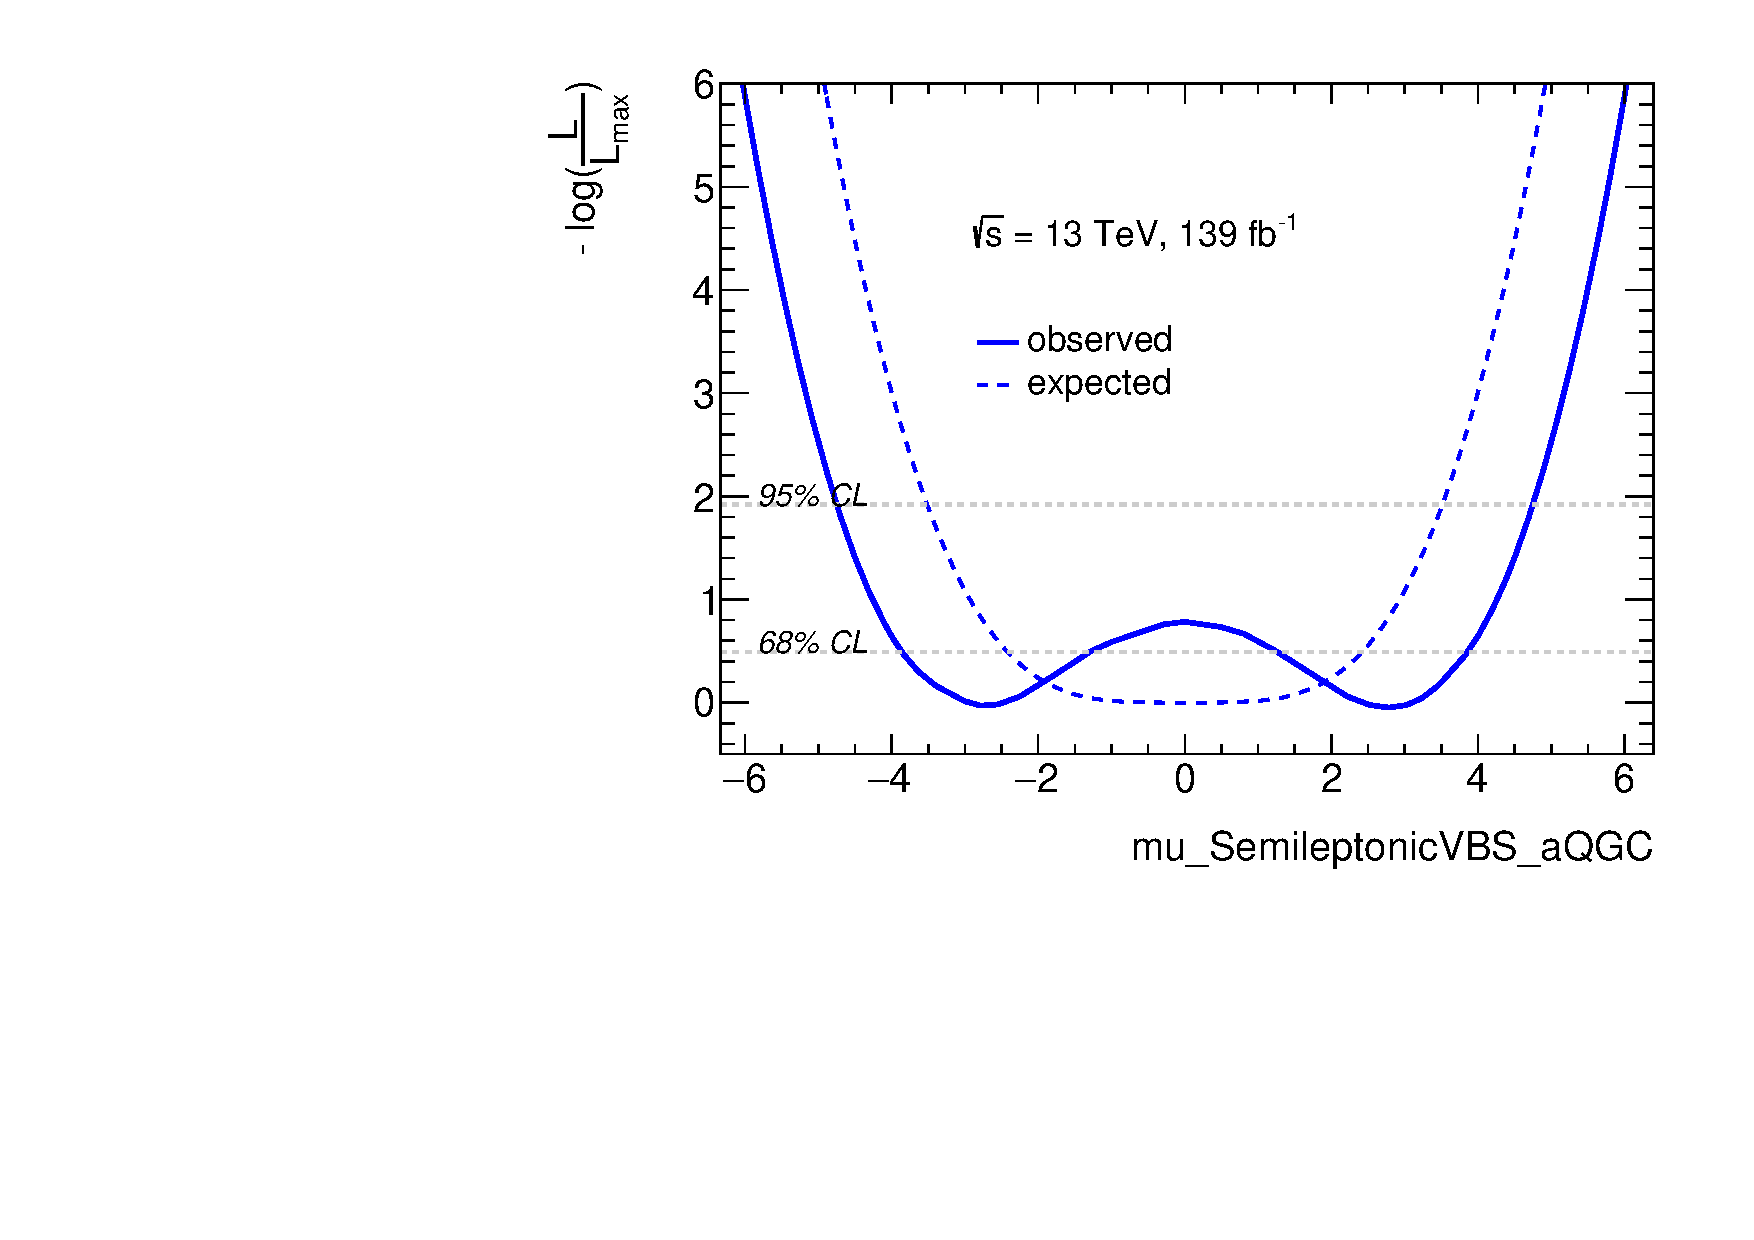
\includegraphics[width=0.38\textwidth]{figures/aQGC/profileFS023000}
        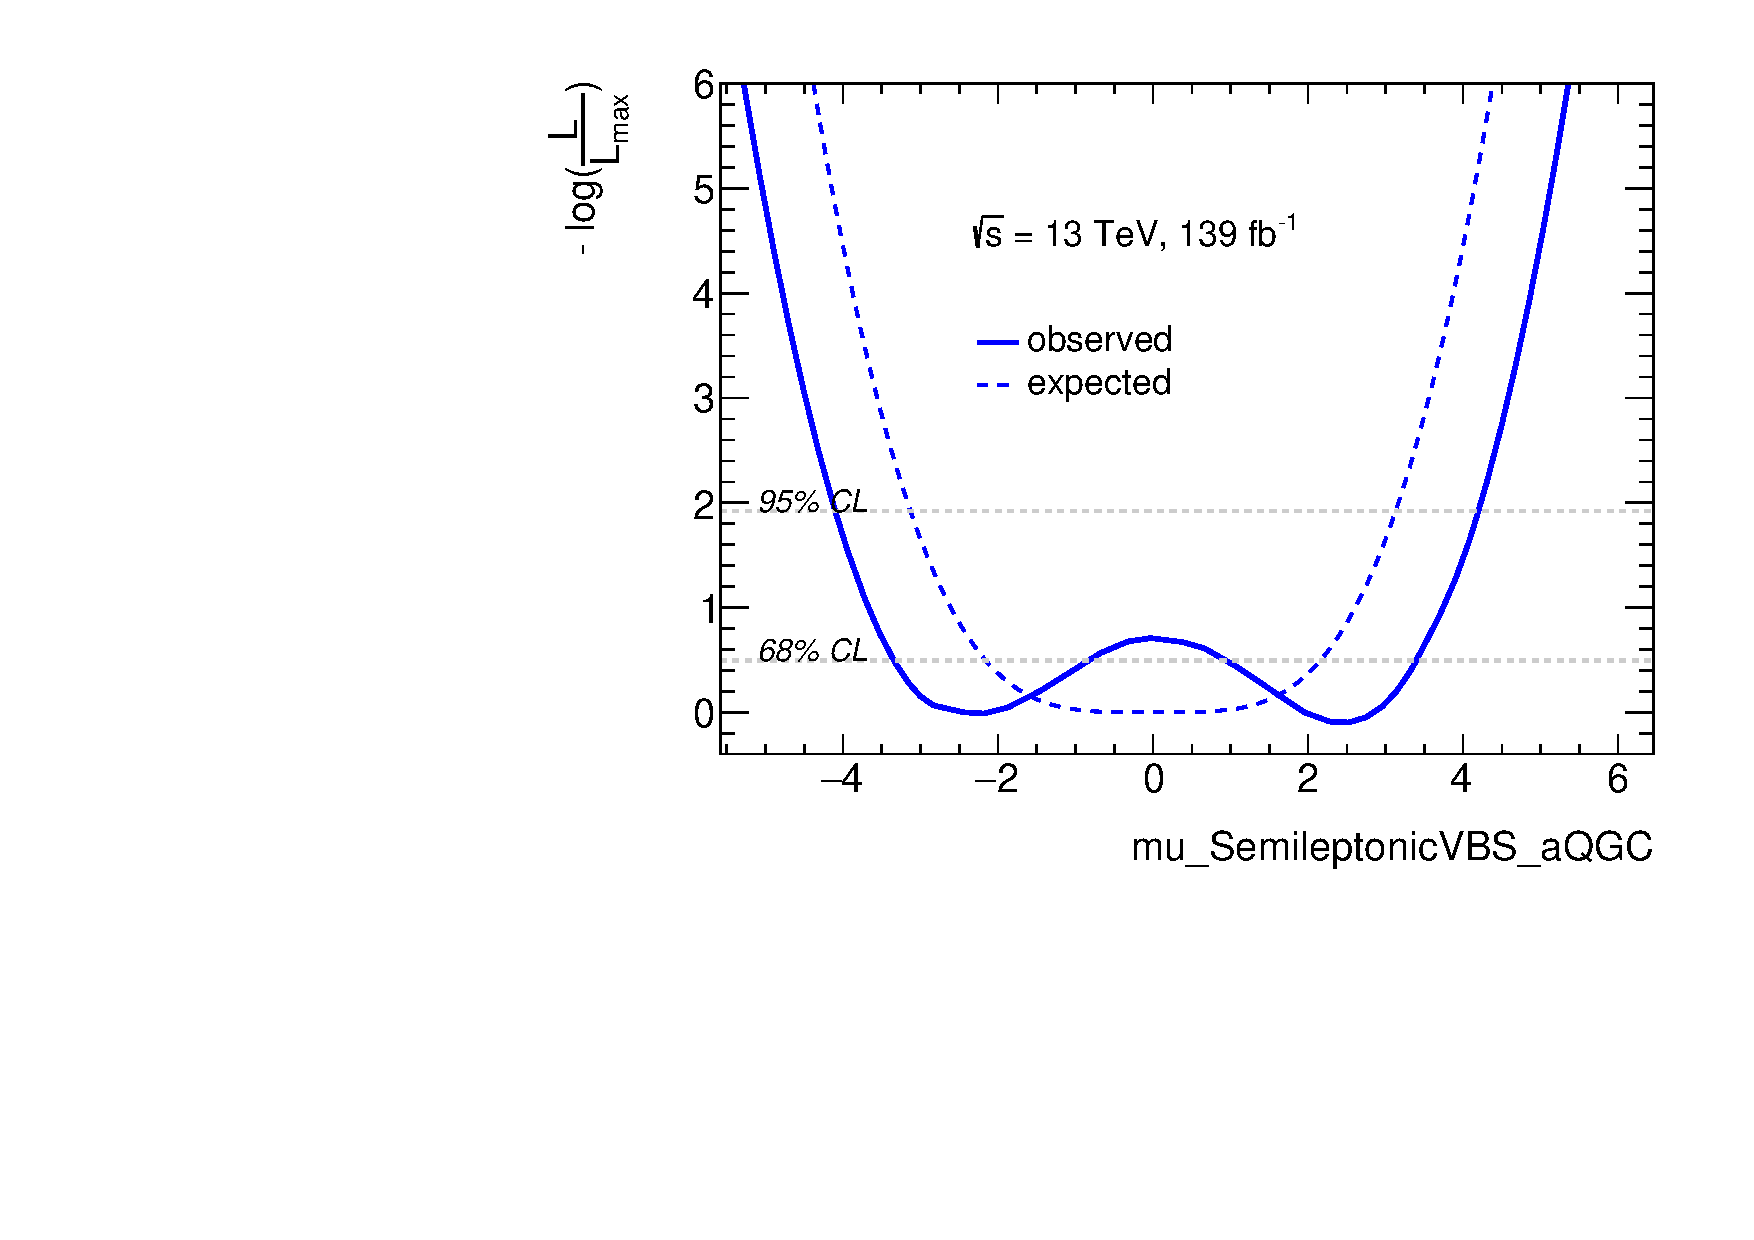
\includegraphics[width=0.32\textwidth]{figures/aQGC/profileFS02inf}
        \caption{The observed log-likelihood curves of FS02 Wilson coefficient where the clipping energy is 1.5~TeV (left), 2.0~TeV (middle), $\infty$ (right).}
        \label{fig:ProfileLL}
\end{figure}
\begin{figure}[ht]
    \centering
    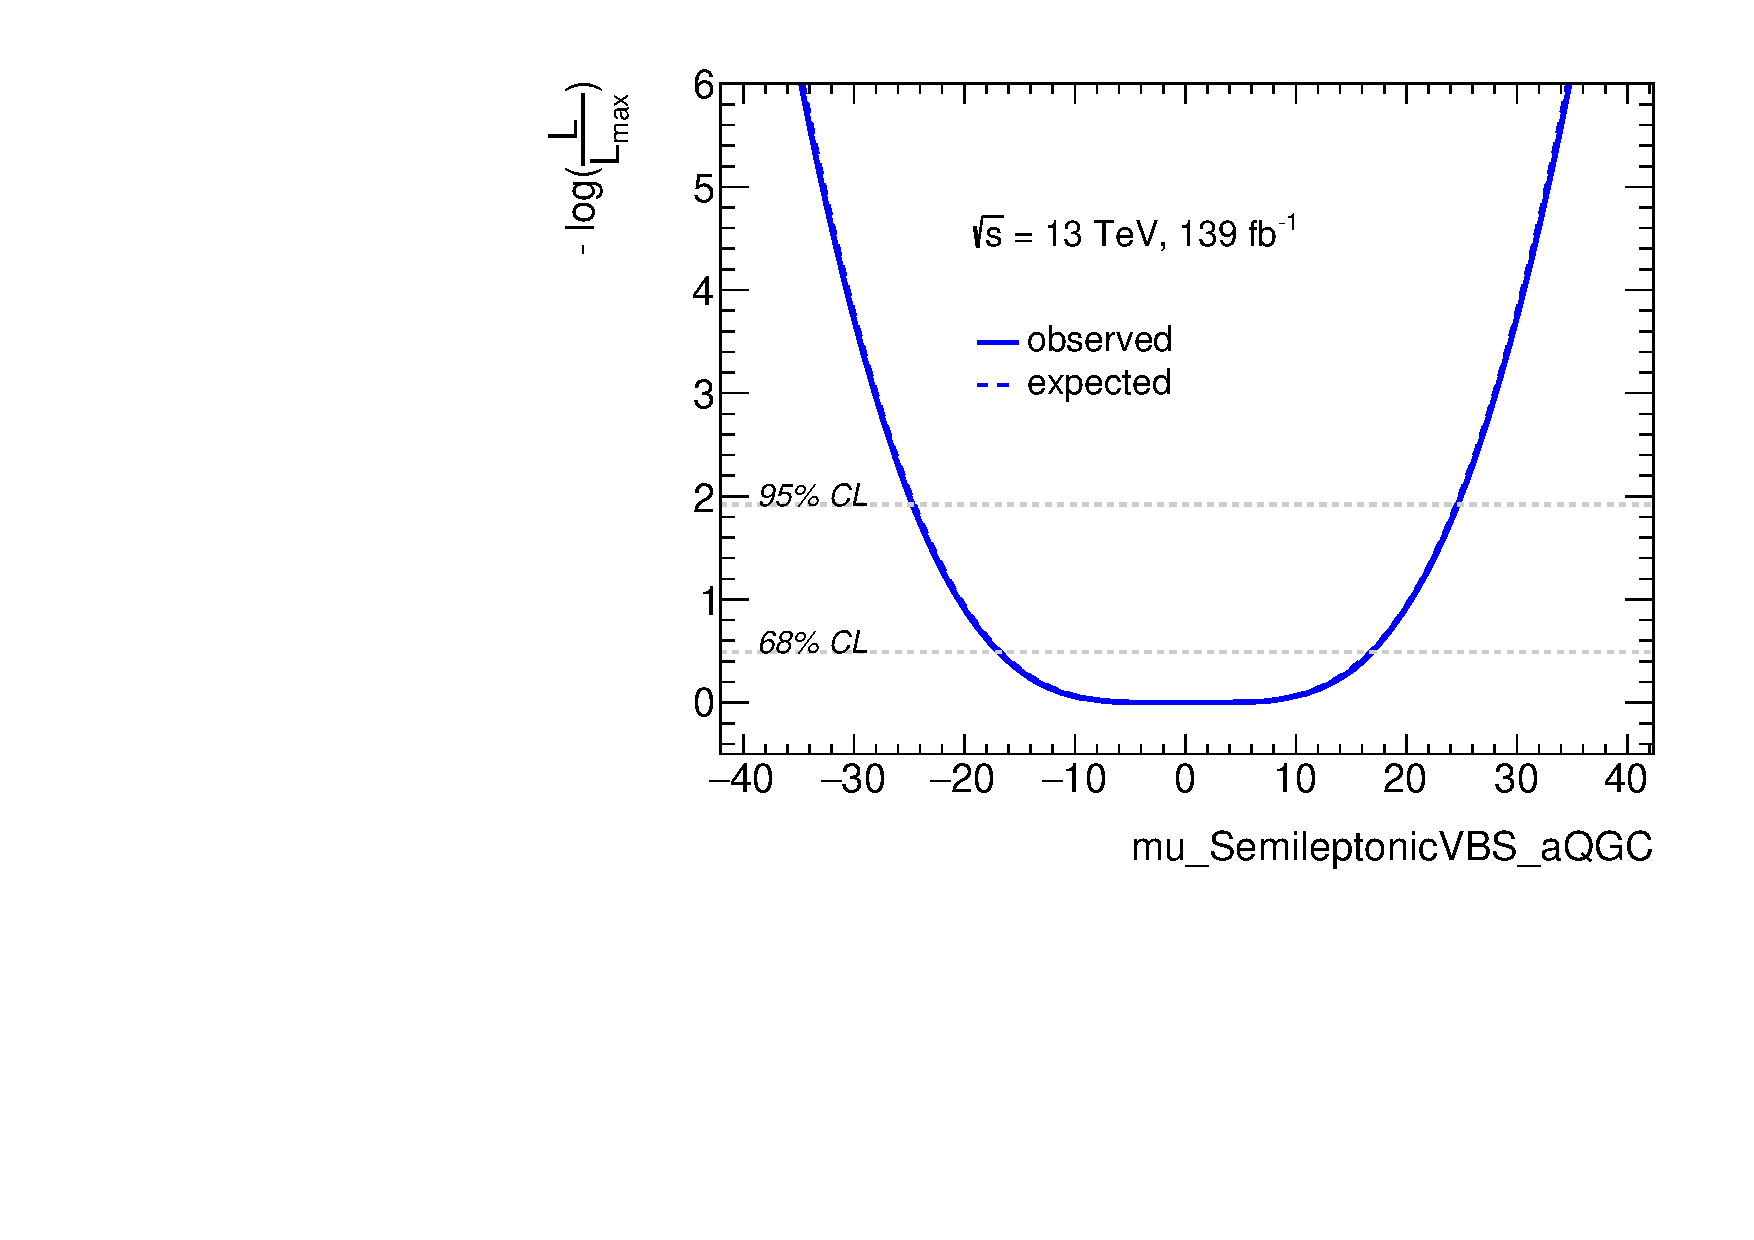
\includegraphics[width=0.32\textwidth]{figures/aQGC/profileFS11500}
    	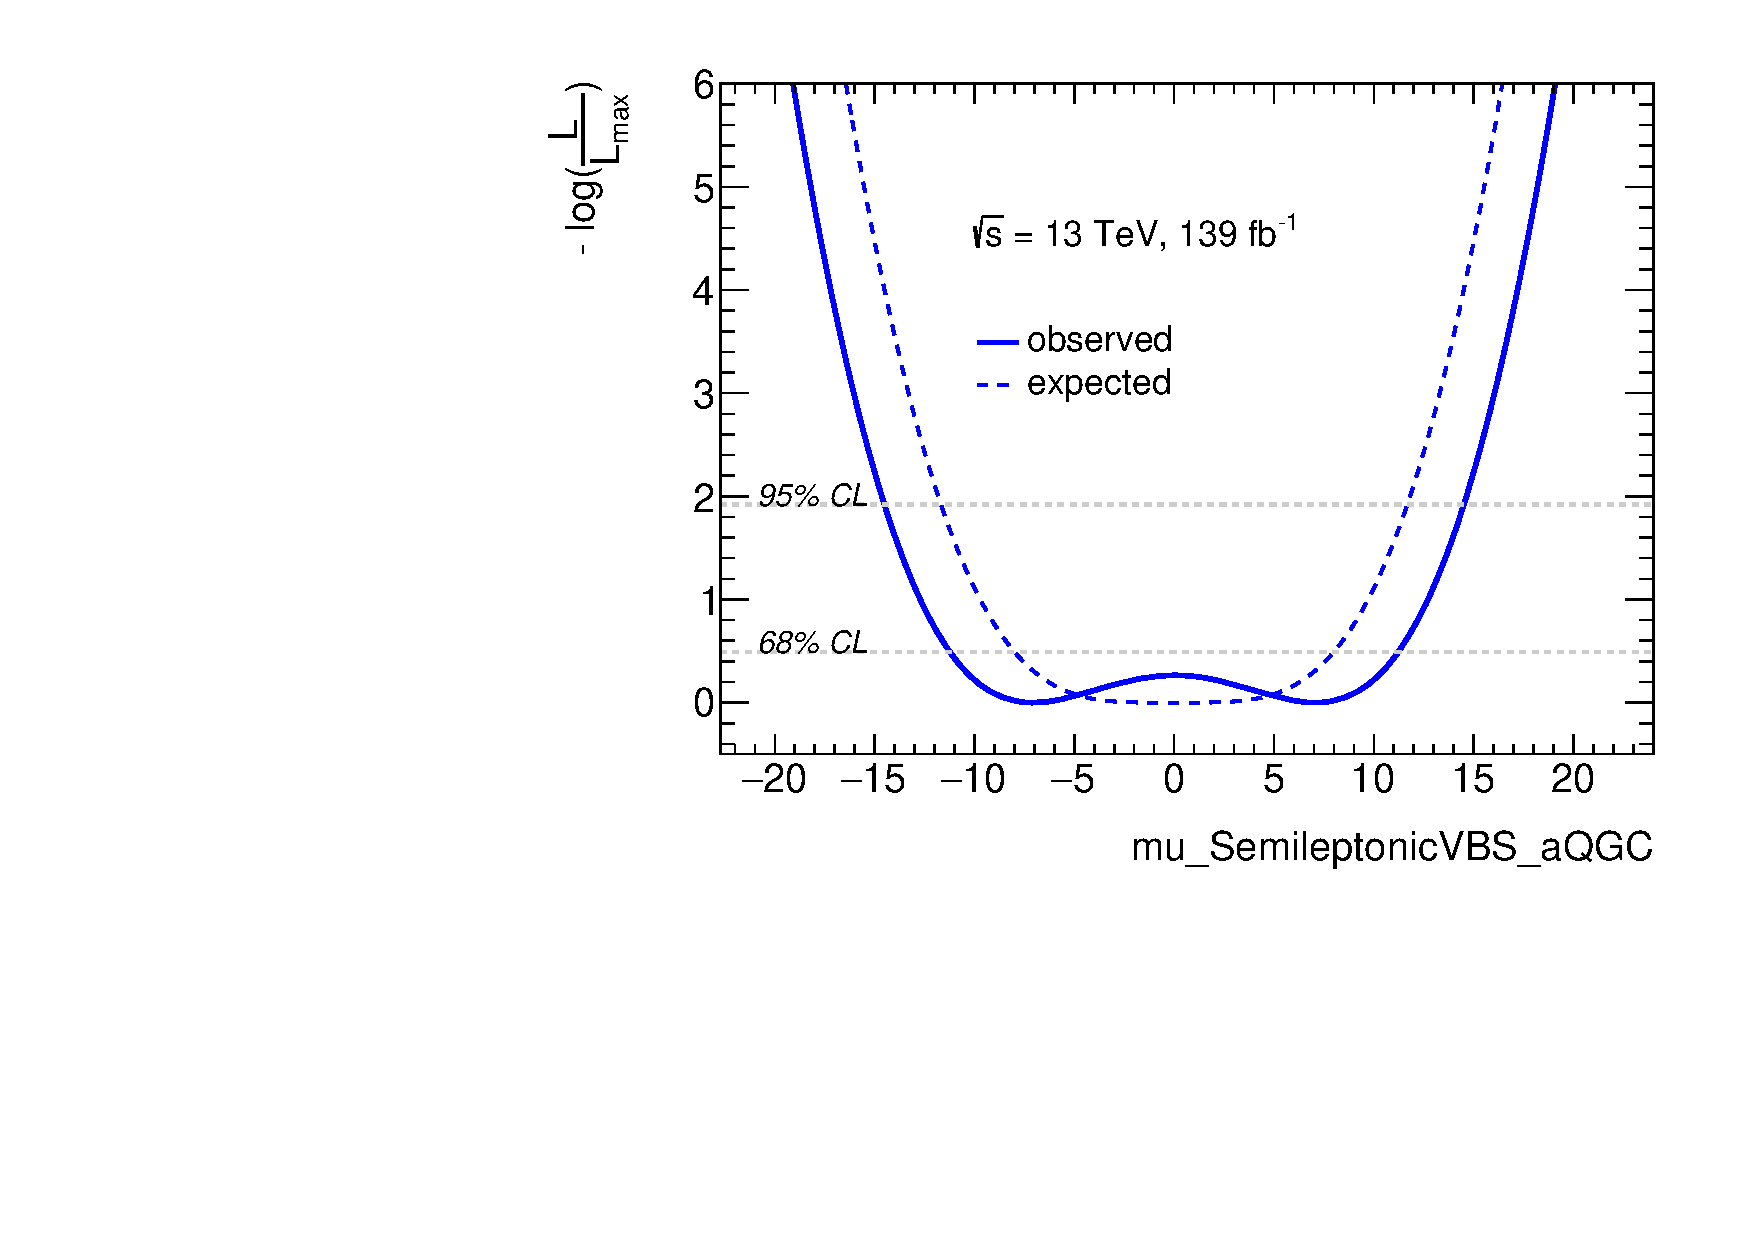
\includegraphics[width=0.32\textwidth]{figures/aQGC/profileFS12000}
    	%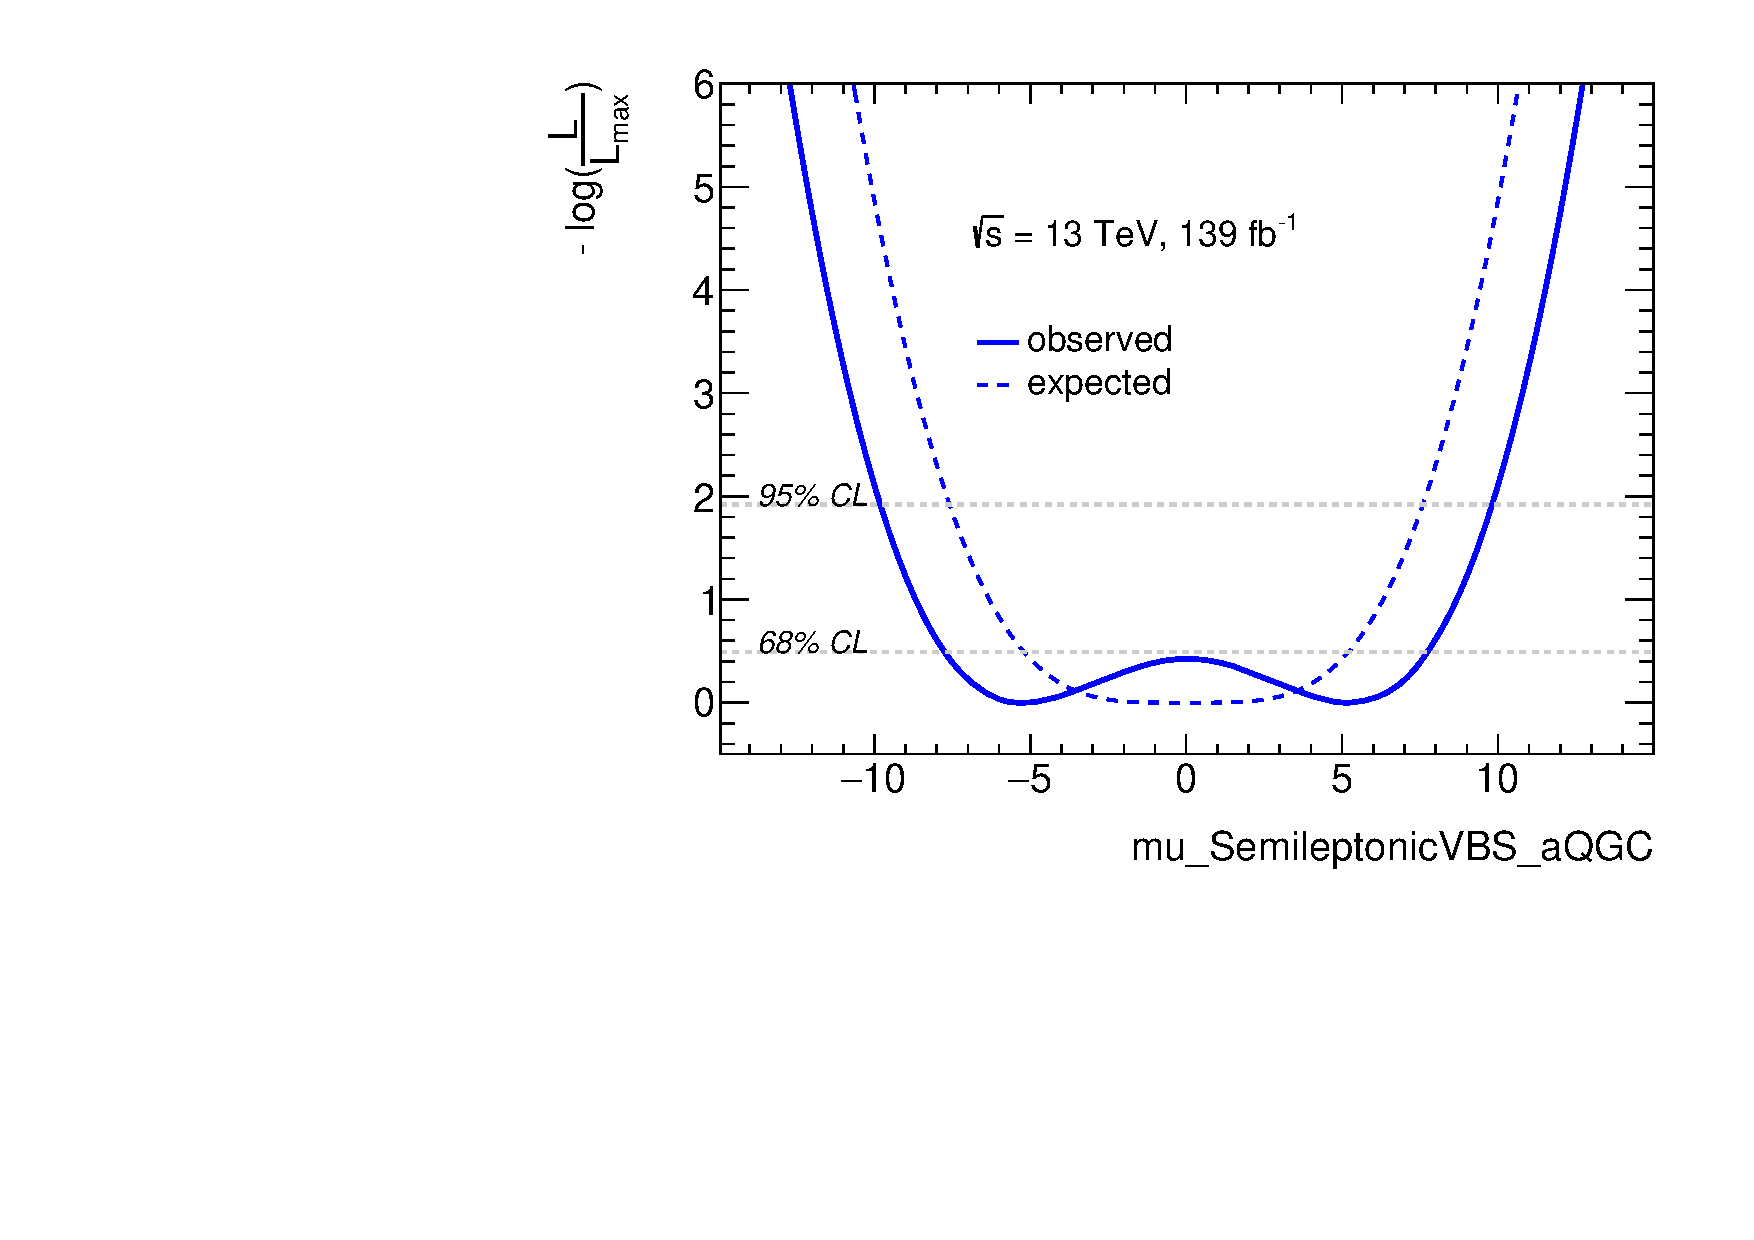
\includegraphics[width=0.38\textwidth]{figures/aQGC/profileFS13000}
        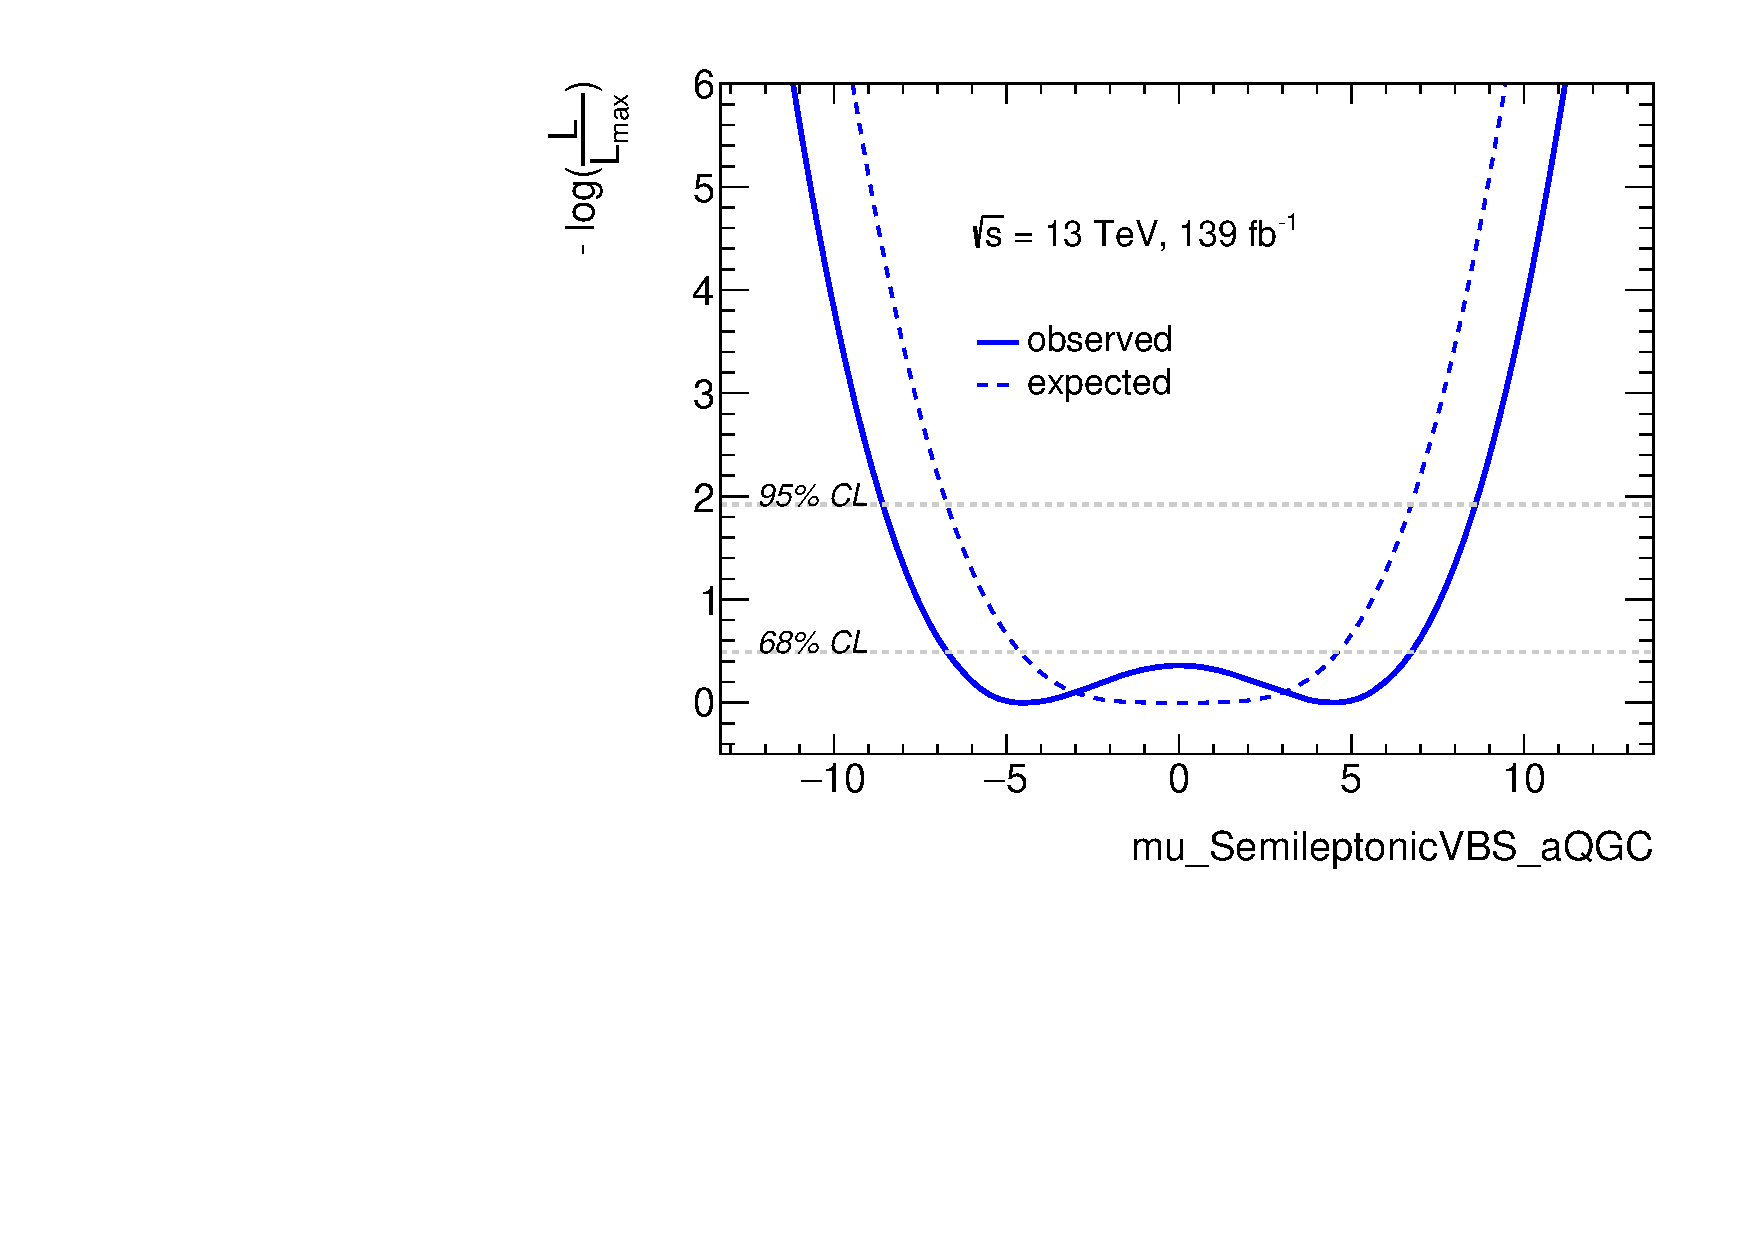
\includegraphics[width=0.32\textwidth]{figures/aQGC/profileFS1inf}
        \caption{The observed log-likelihood curves of FS1 Wilson coefficient where the clipping energy is 1.5~TeV (left), 2.0~TeV (middle), $\infty$ (right).}
        \label{fig:ProfileLL}
\end{figure}

%FM
\begin{figure}[ht]
    \centering
    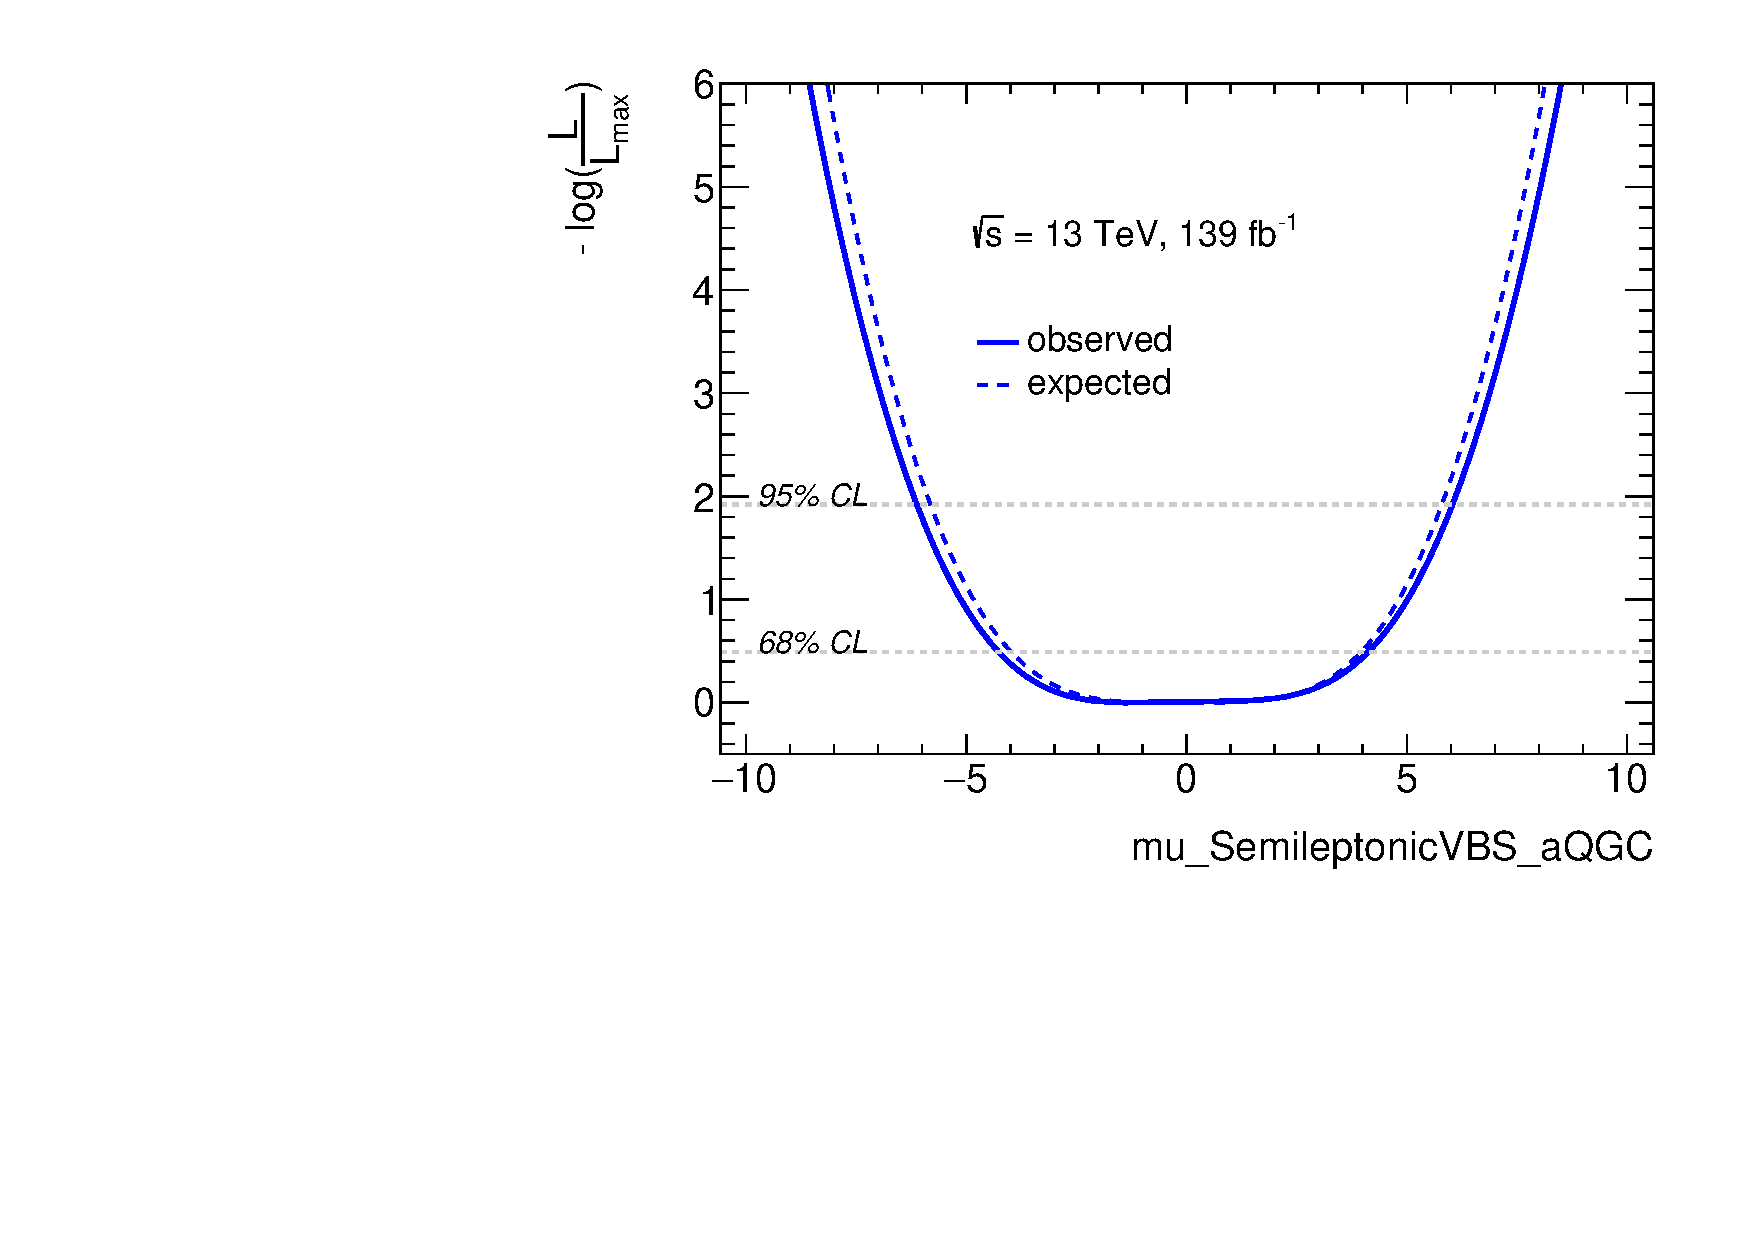
\includegraphics[width=0.32\textwidth]{figures/aQGC/profileFM01500}
    	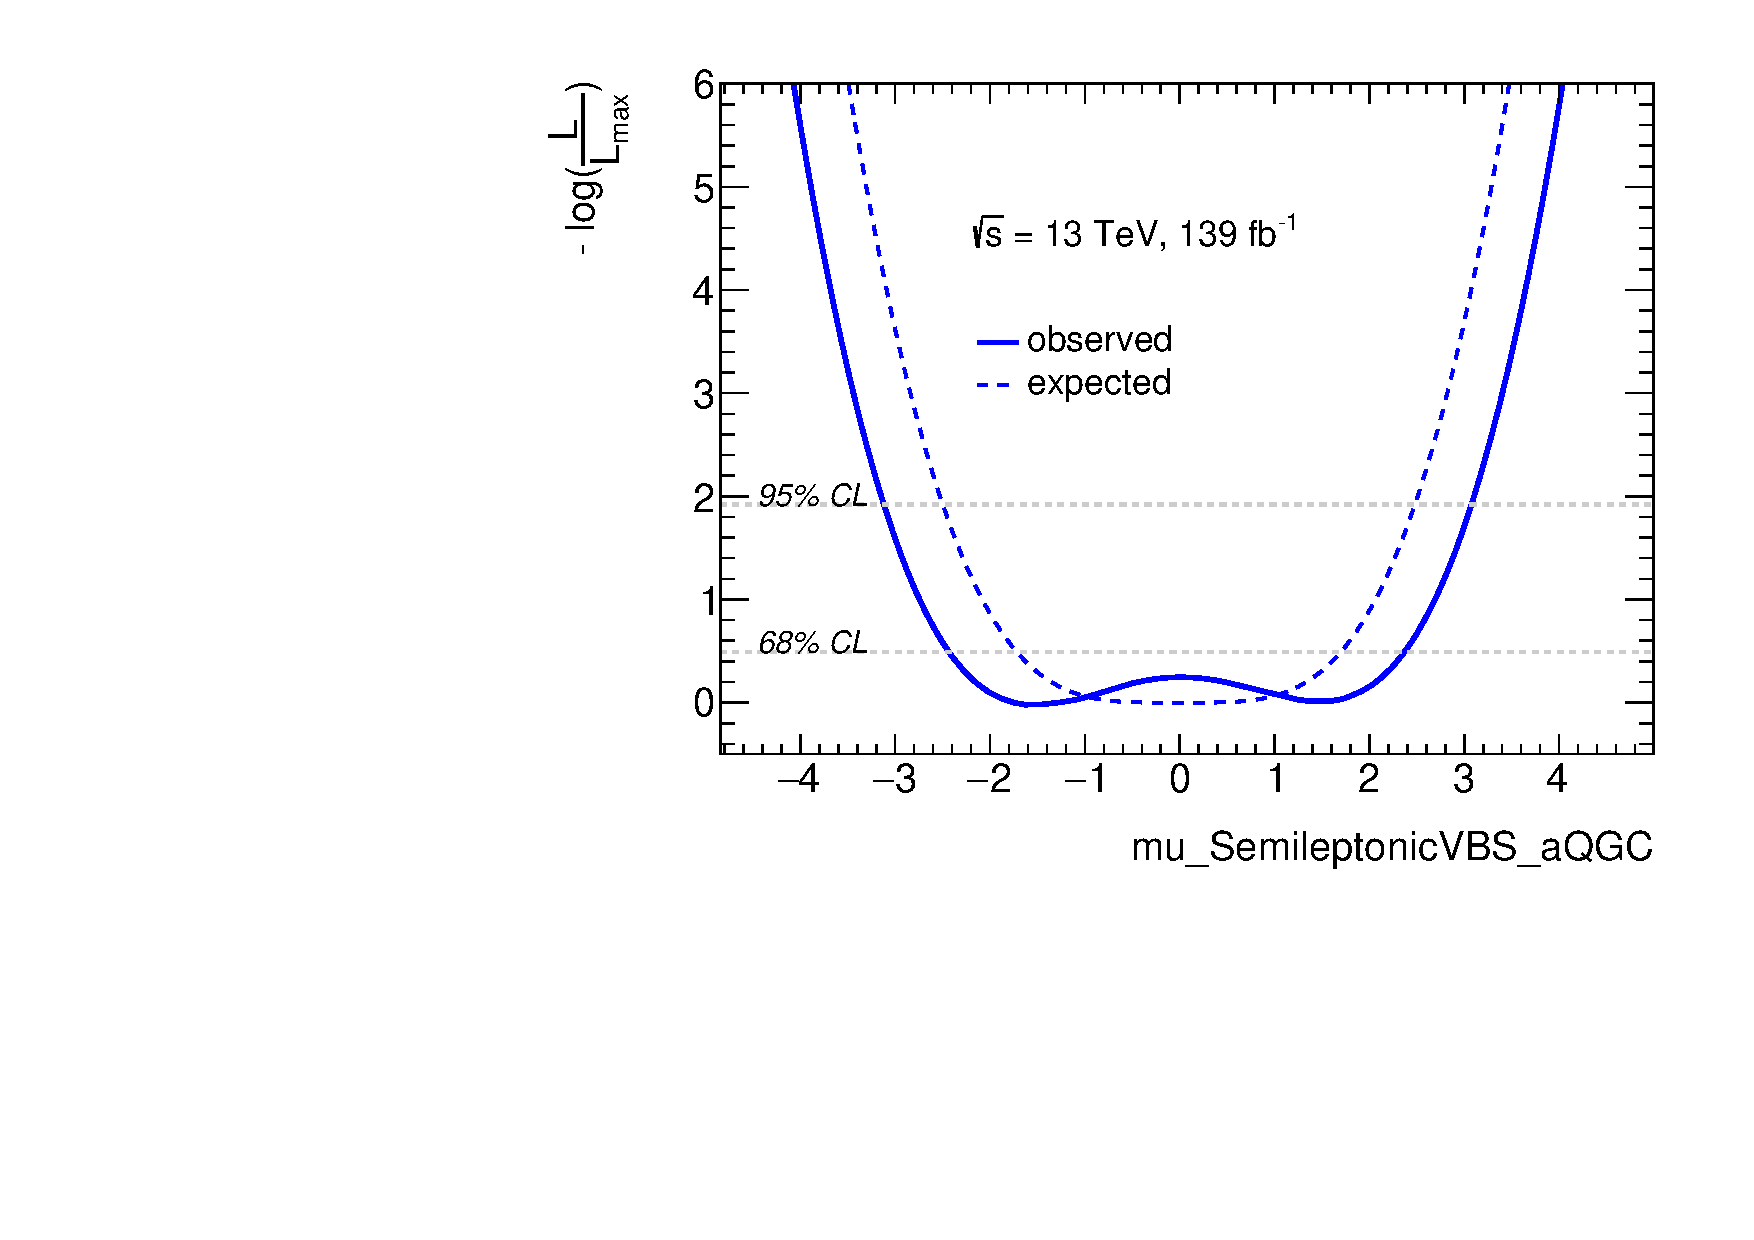
\includegraphics[width=0.32\textwidth]{figures/aQGC/profileFM02000}
    	%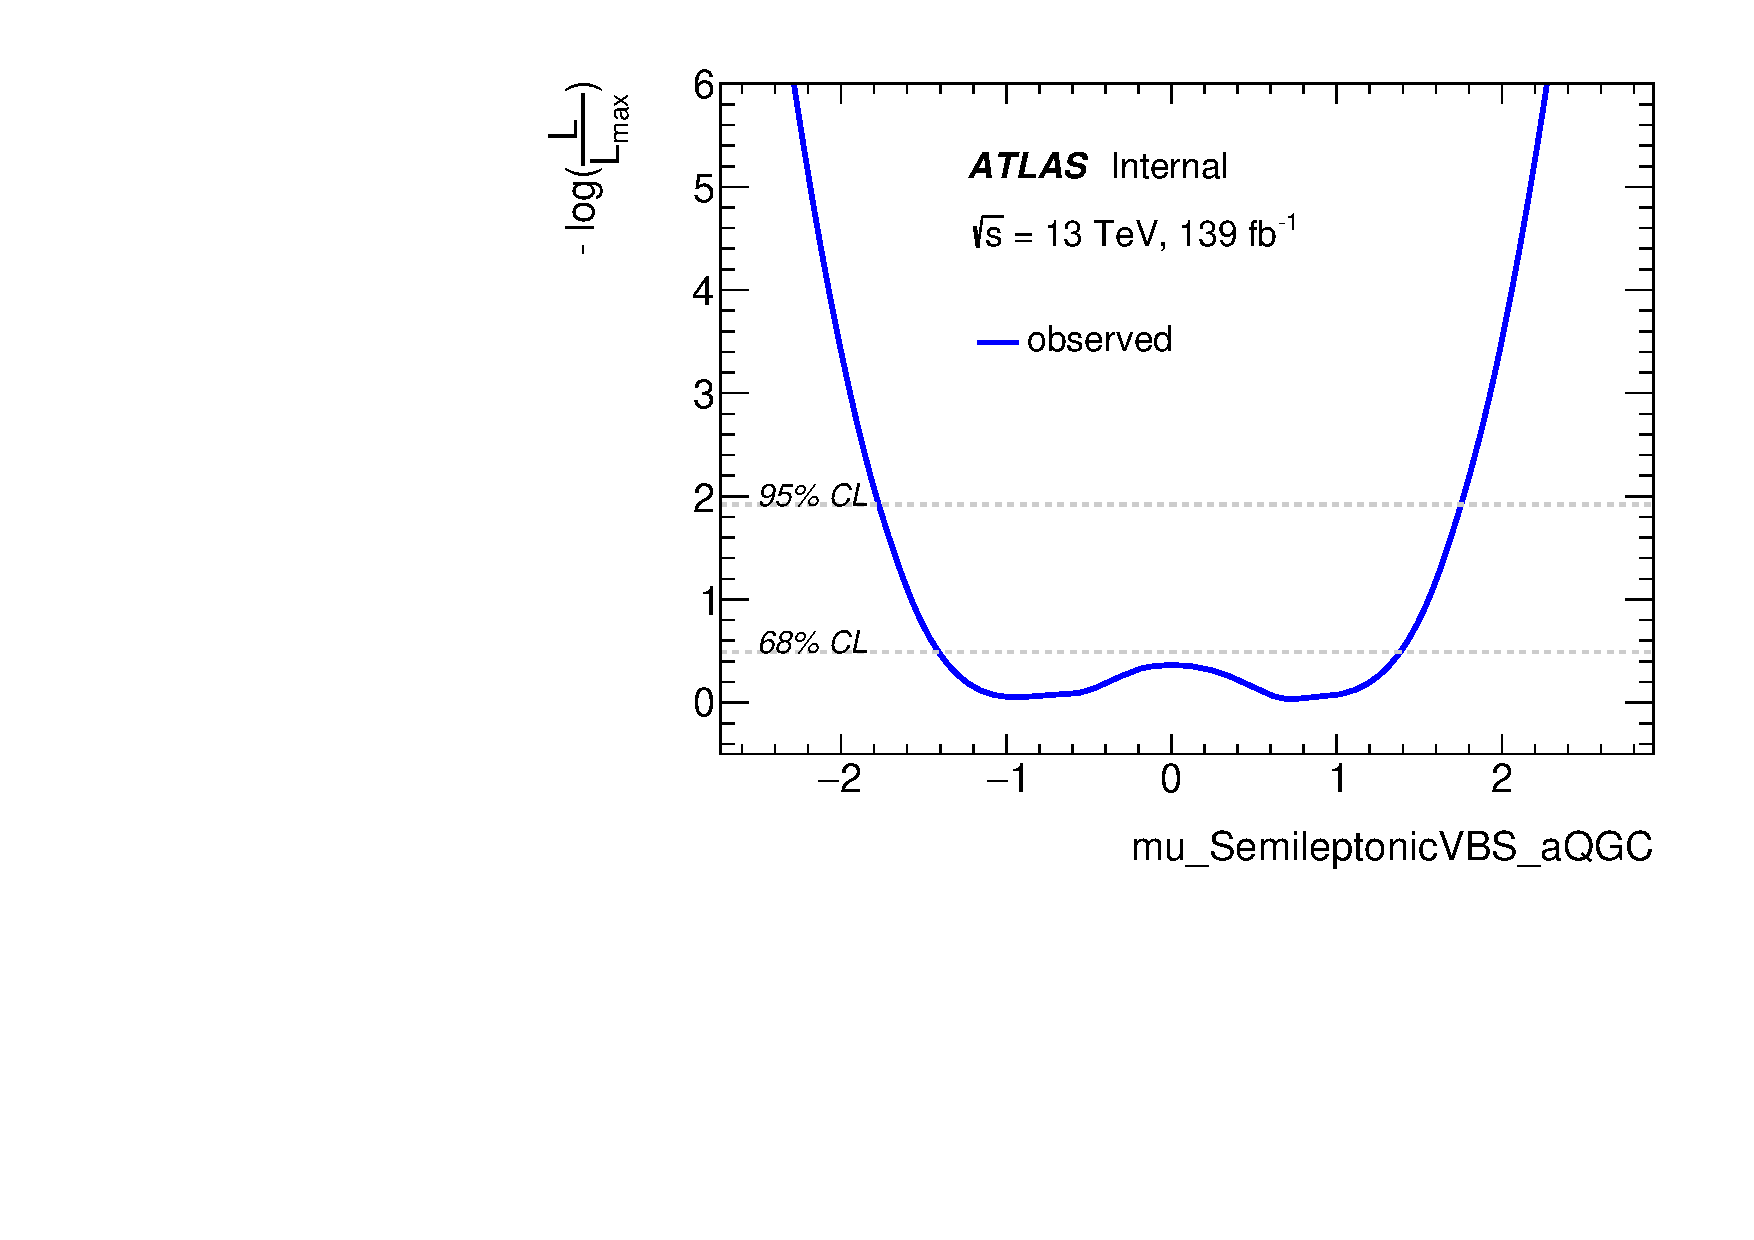
\includegraphics[width=0.38\textwidth]{figures/aQGC/profileFM03000}
        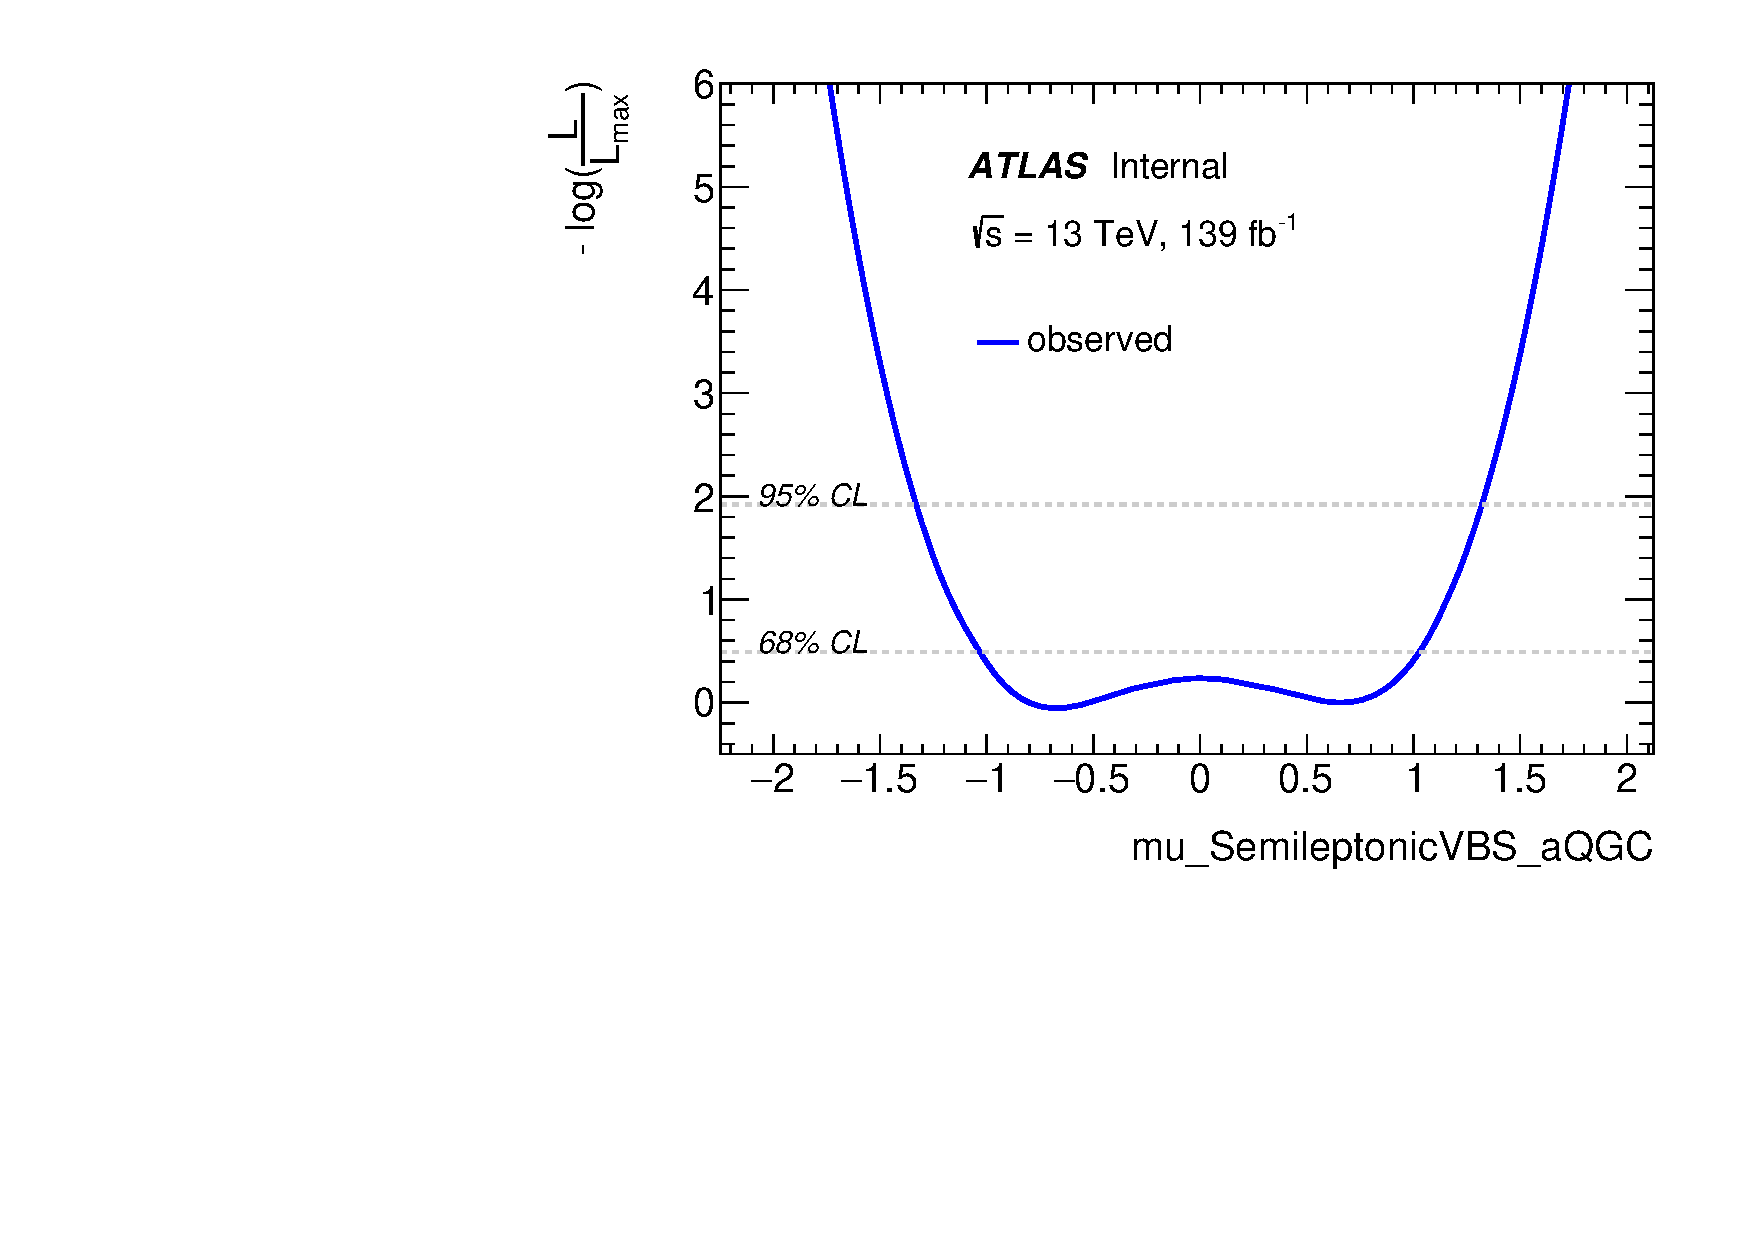
\includegraphics[width=0.32\textwidth]{figures/aQGC/profileFM0inf}
        \caption{The observed log-likelihood curves of FM0 Wilson coefficient where the clipping energy is 1.5~TeV (left), 2.0~TeV (middle), $\infty$ (right).}
        \label{fig:ProfileLL}
\end{figure}
\begin{figure}[ht]
    \centering
    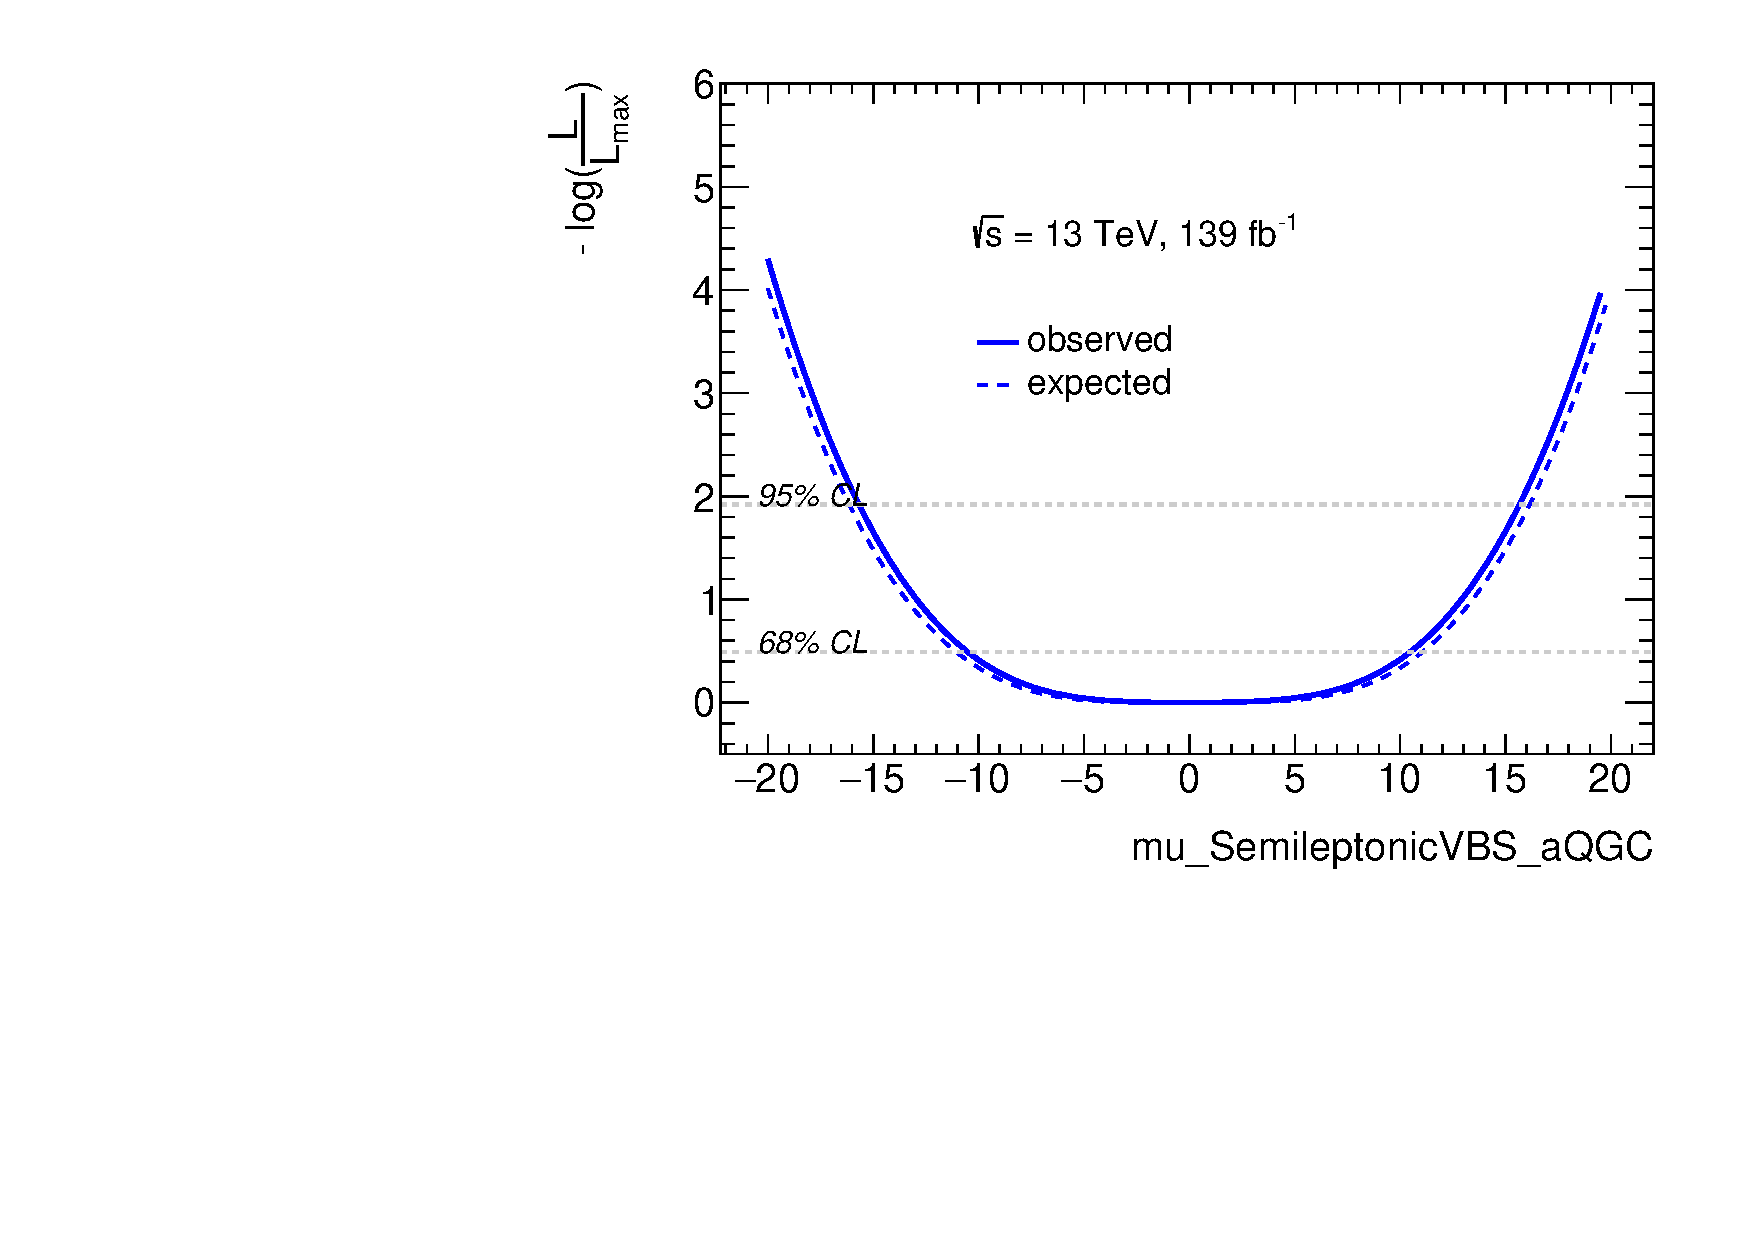
\includegraphics[width=0.32\textwidth]{figures/aQGC/profileFM11500}
    	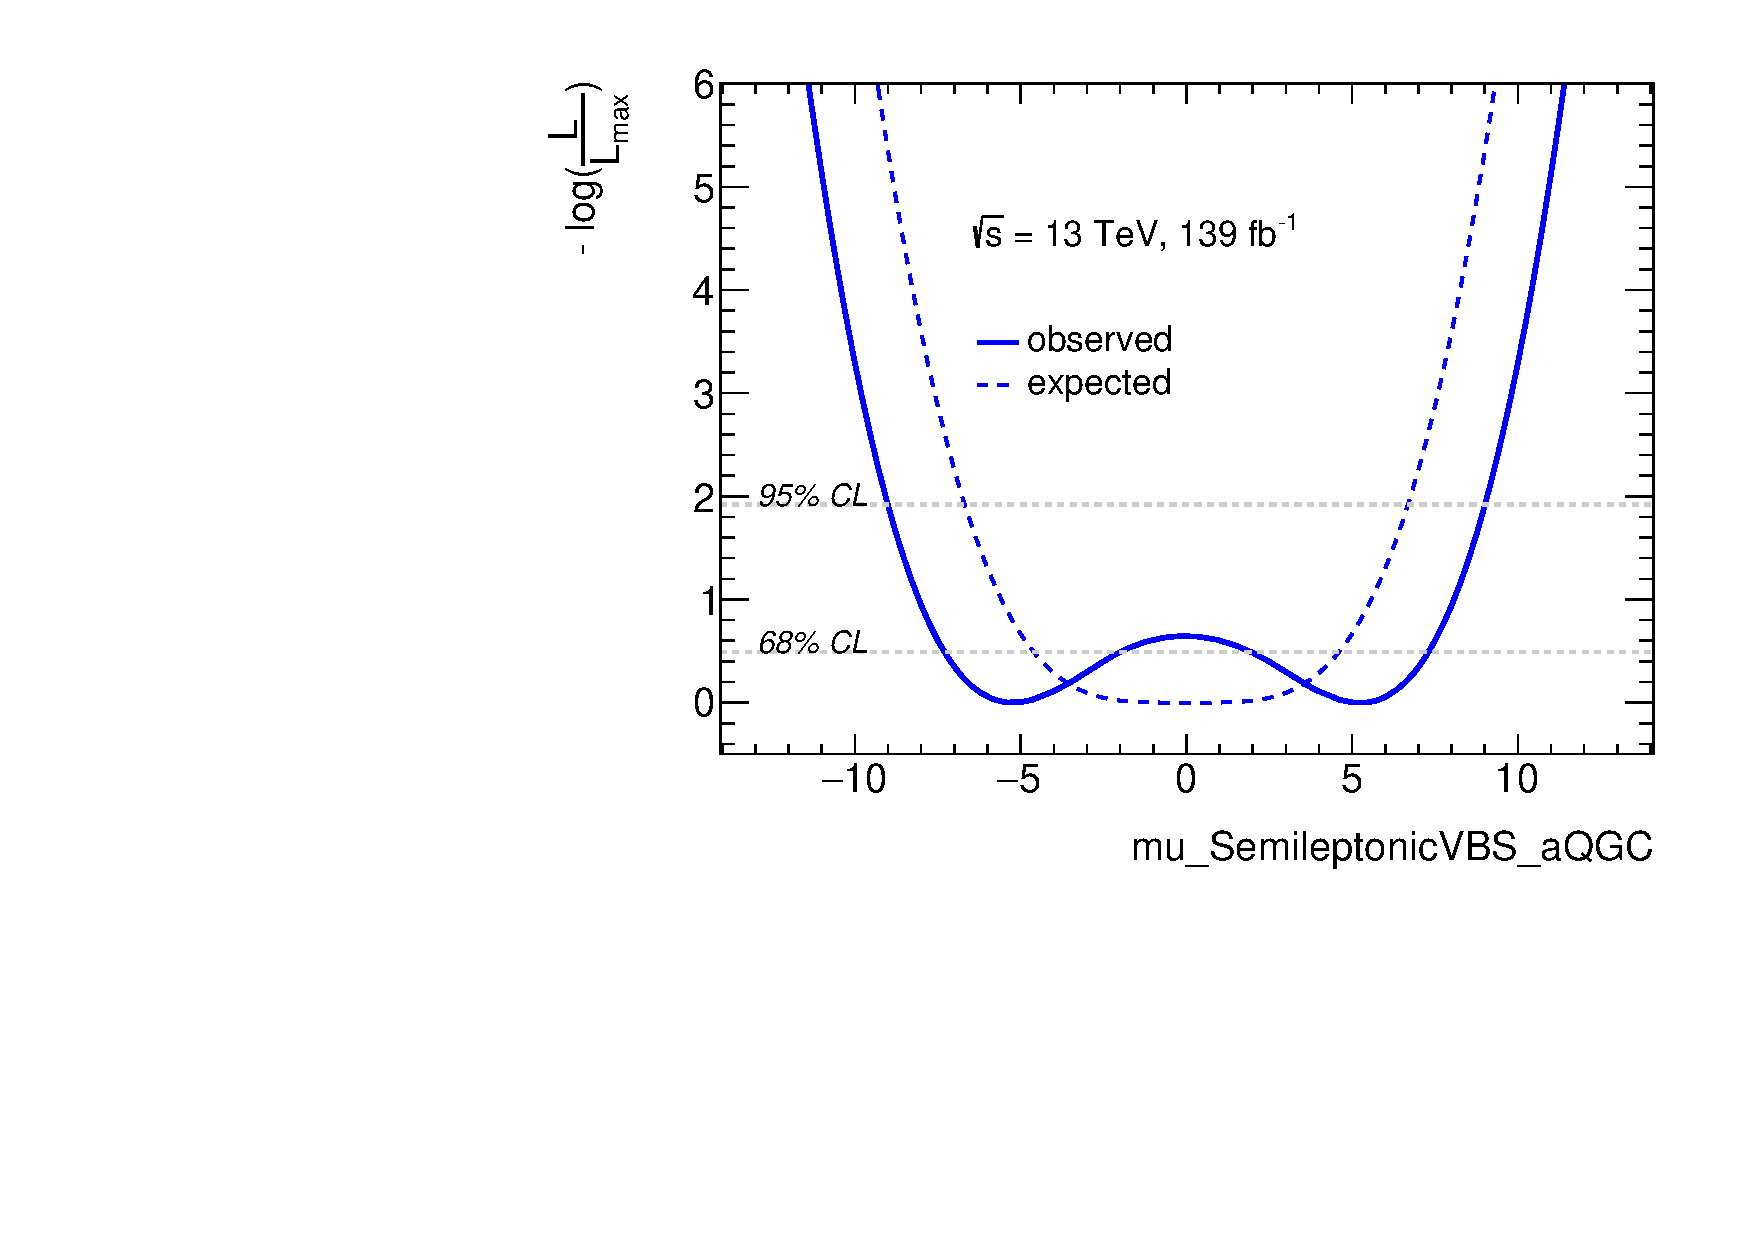
\includegraphics[width=0.32\textwidth]{figures/aQGC/profileFM12000}
    	%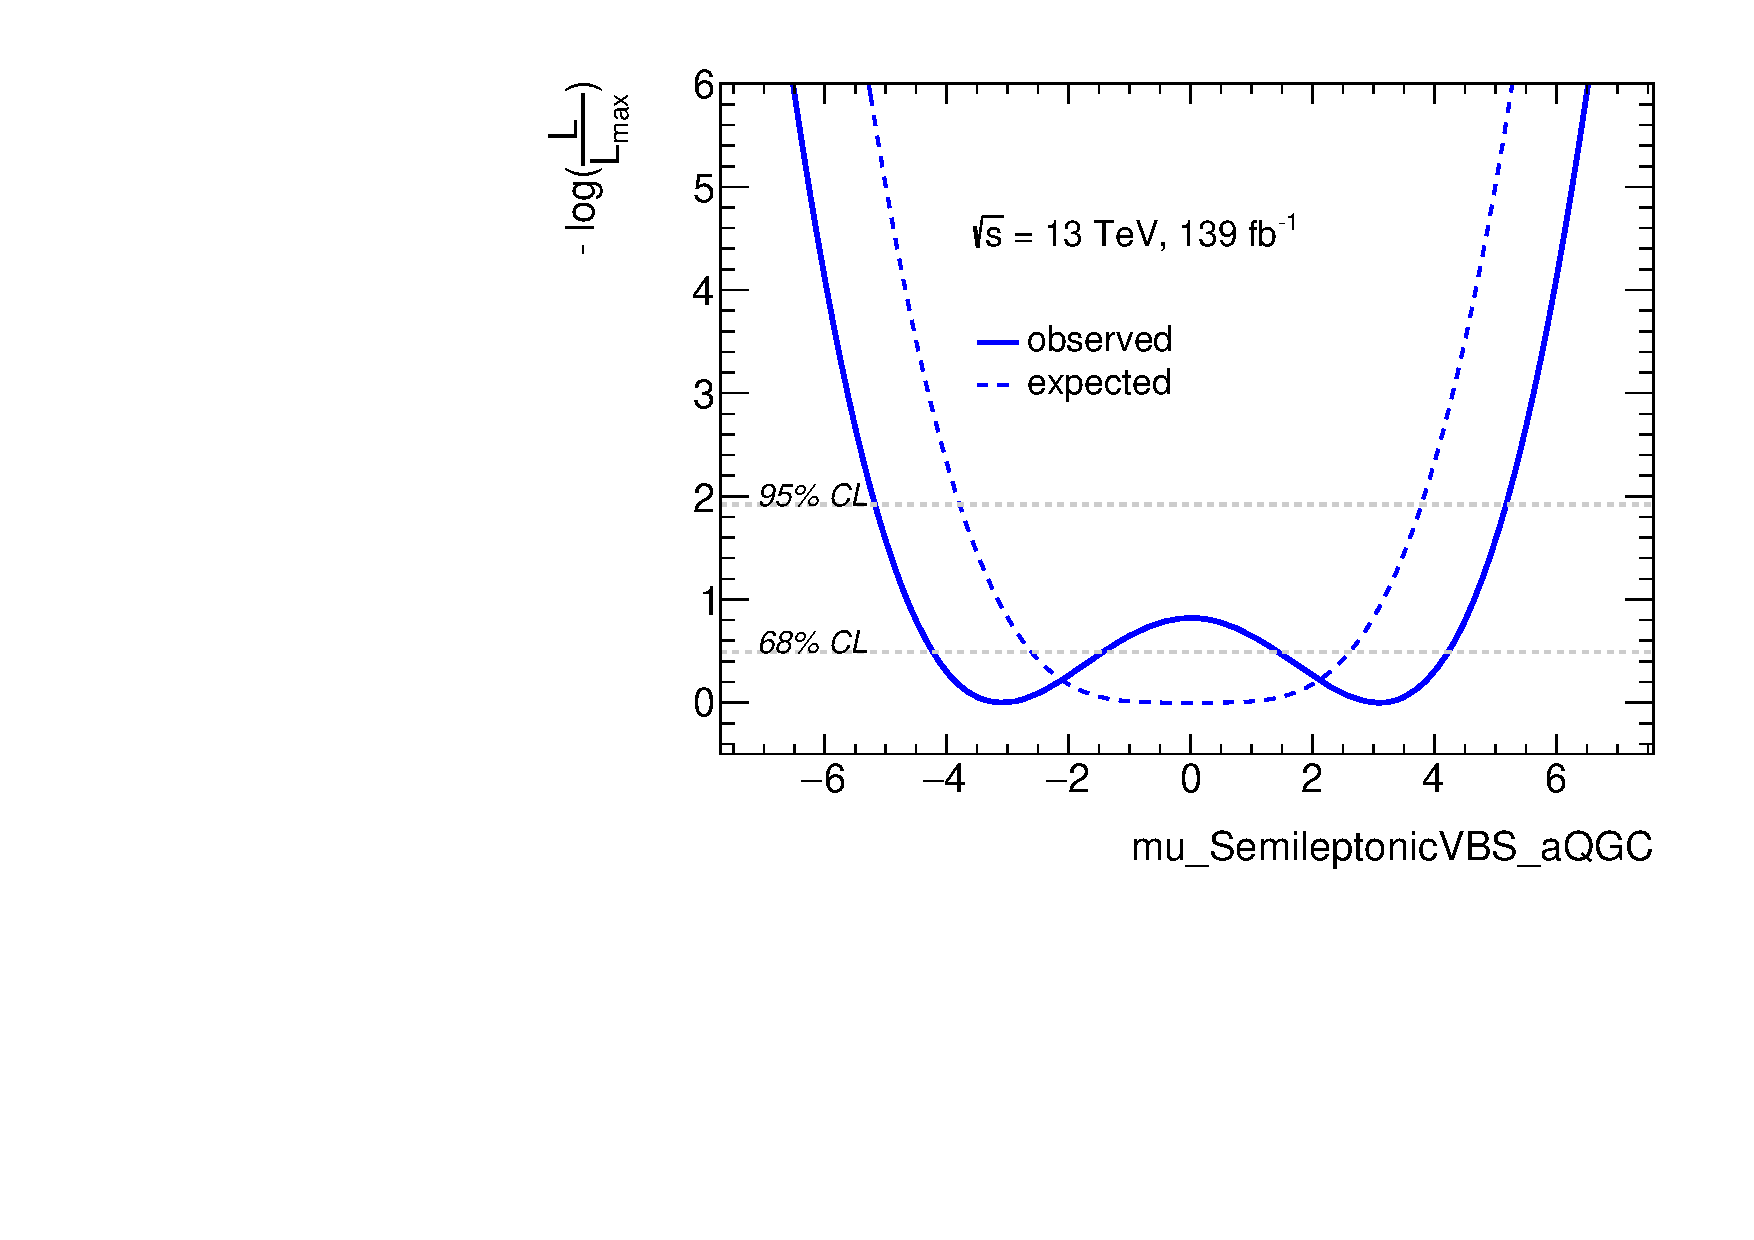
\includegraphics[width=0.38\textwidth]{figures/aQGC/profileFM13000}
        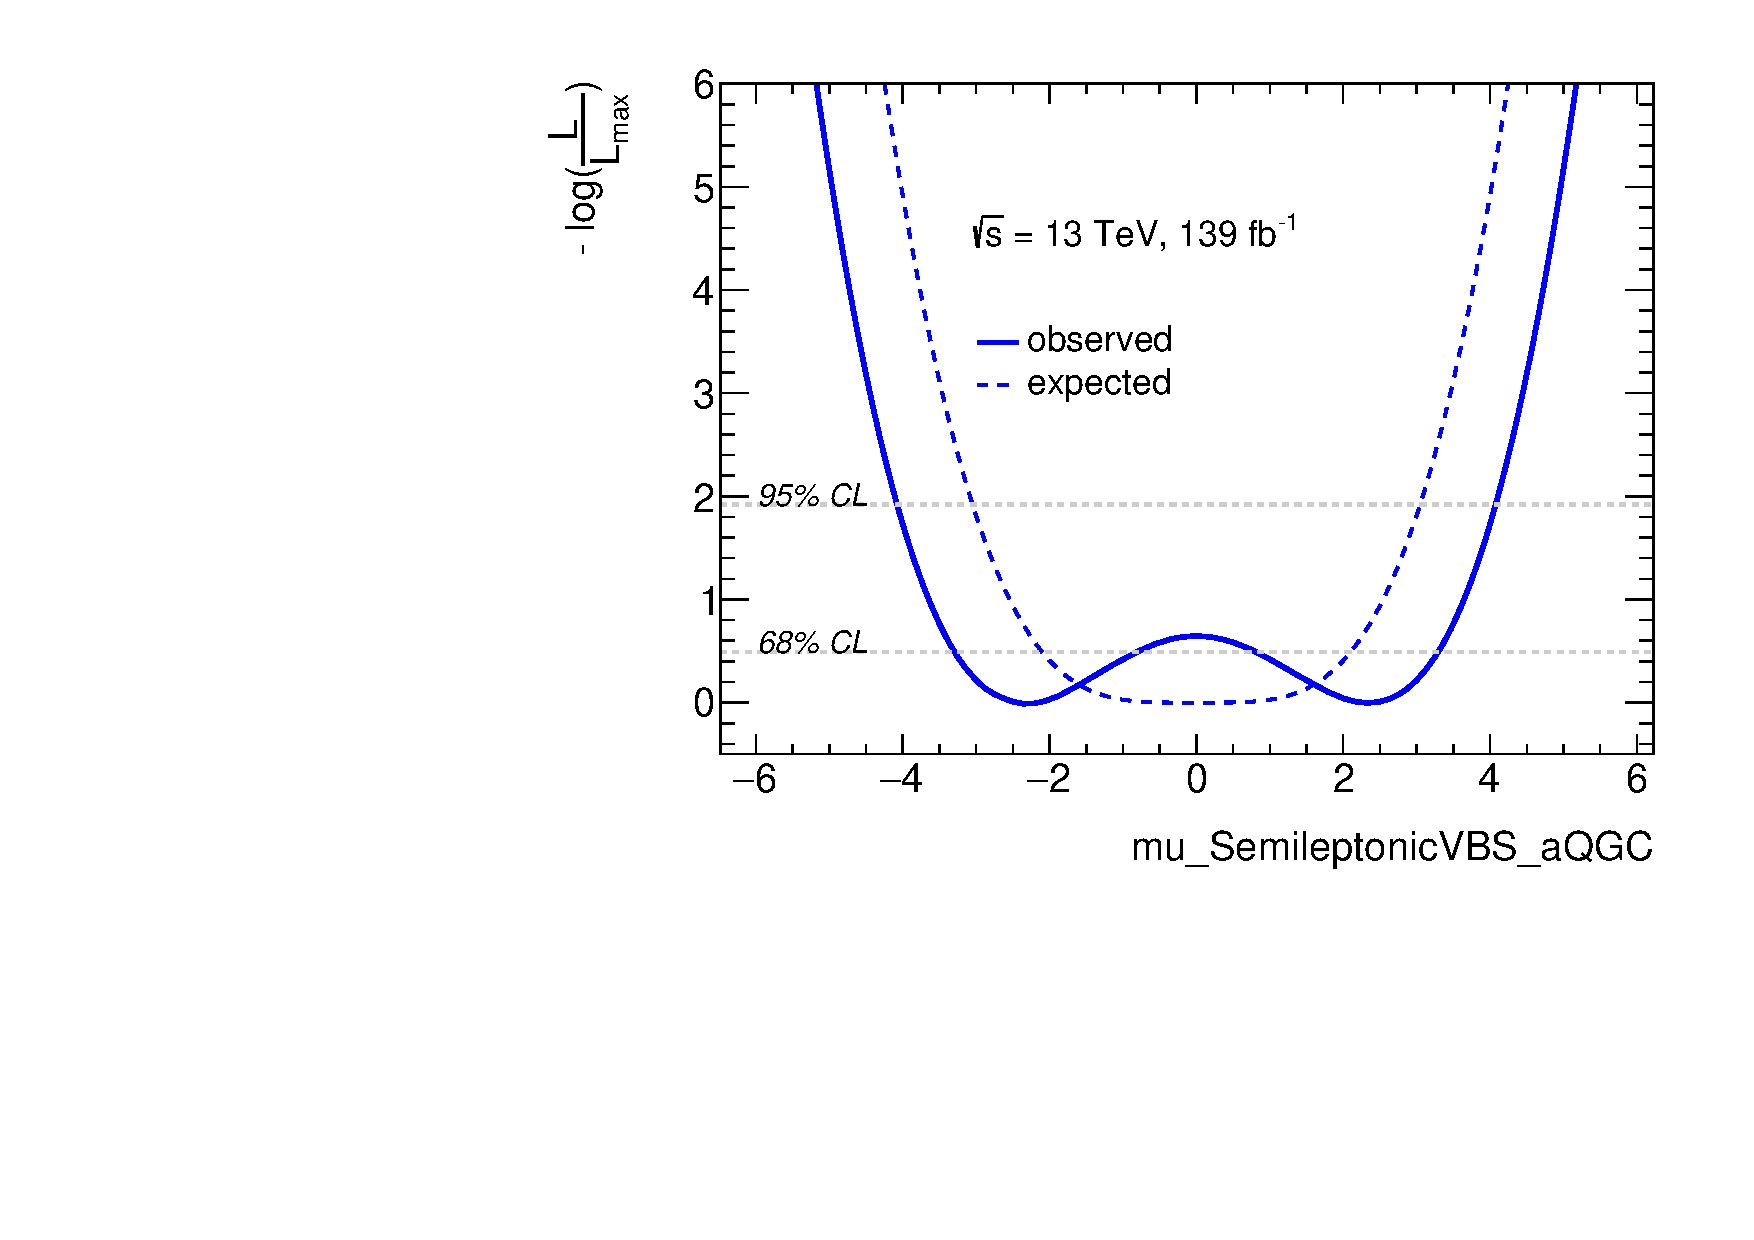
\includegraphics[width=0.32\textwidth]{figures/aQGC/profileFM1inf}
        \caption{The observed log-likelihood curves of FM1 Wilson coefficient where the clipping energy is 1.5~TeV (left), 2.0~TeV (middle), $\infty$ (right).}
        \label{fig:ProfileLL}
\end{figure}
\begin{figure}[ht]
    \centering
    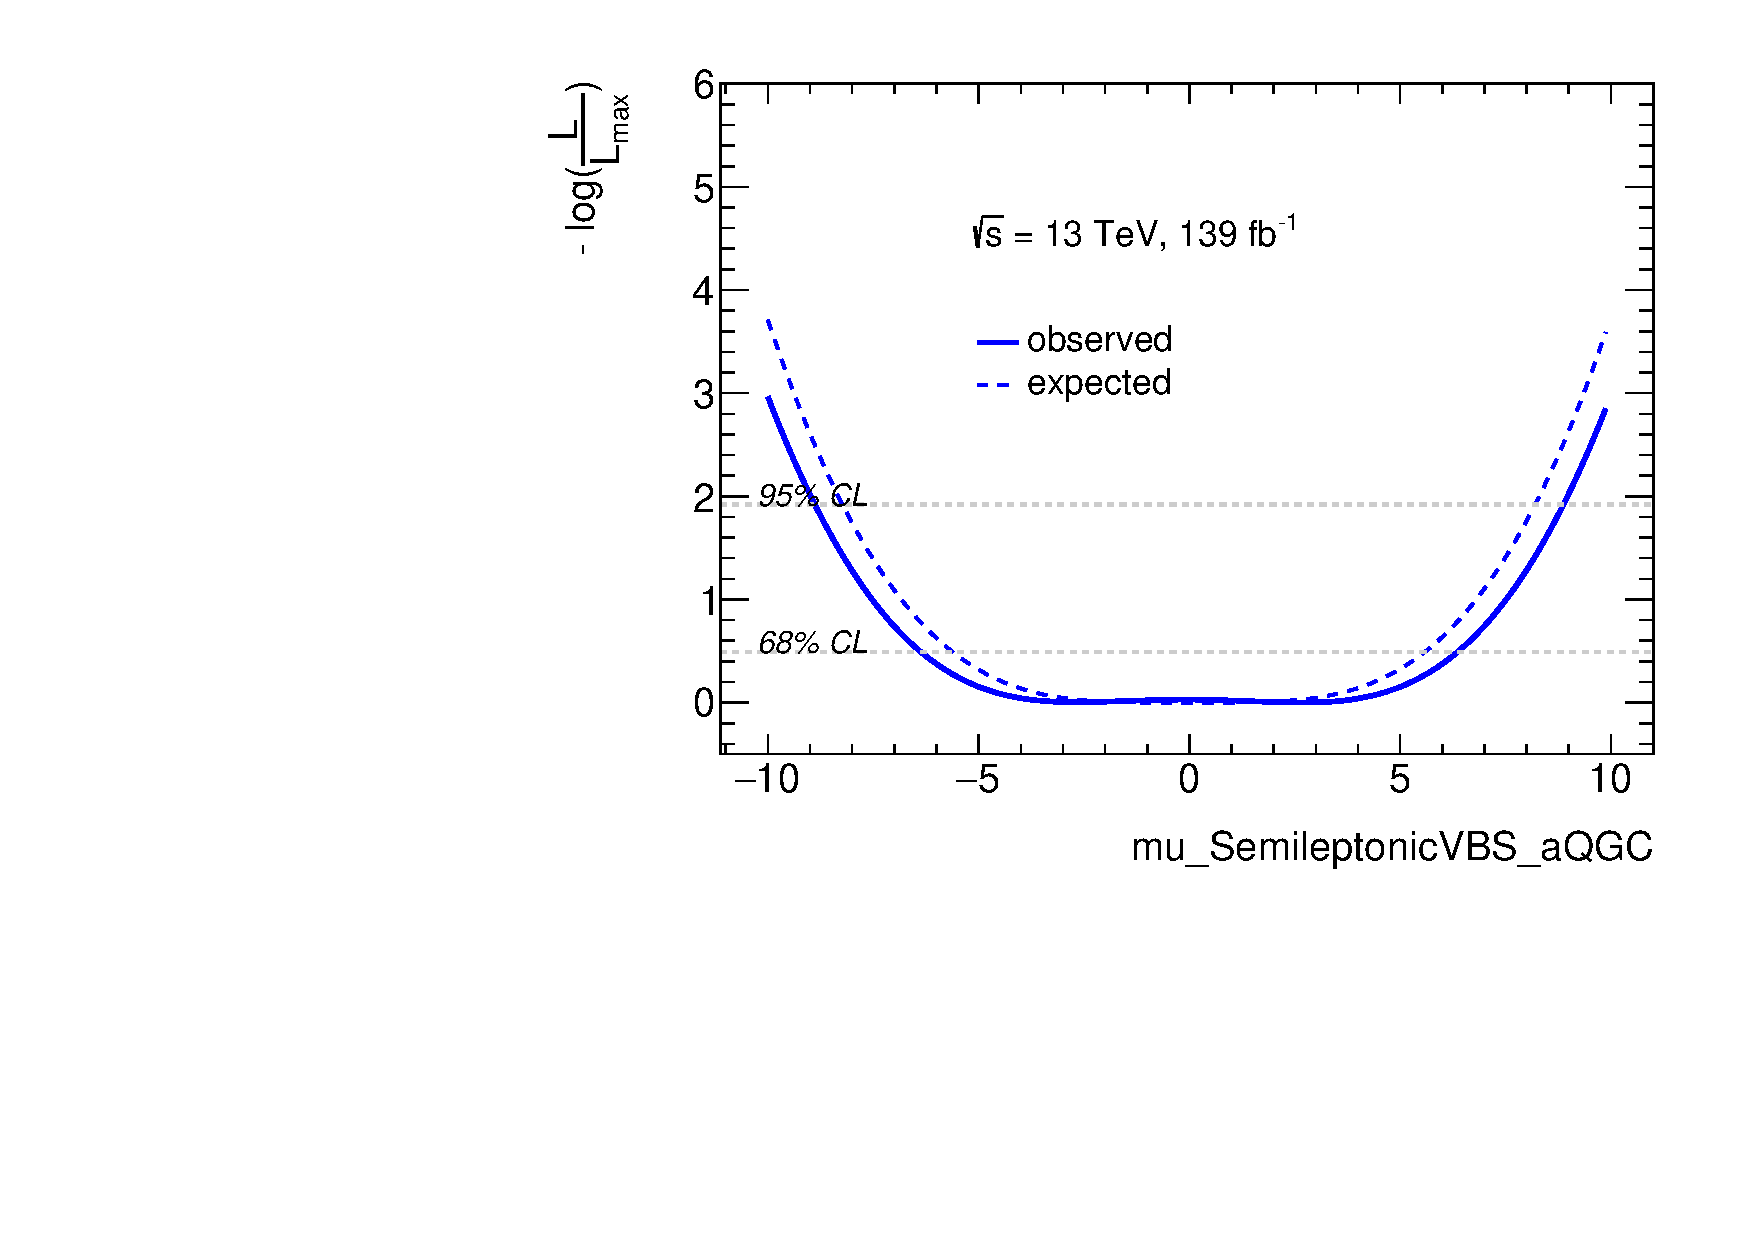
\includegraphics[width=0.32\textwidth]{figures/aQGC/profileFM21500}
    	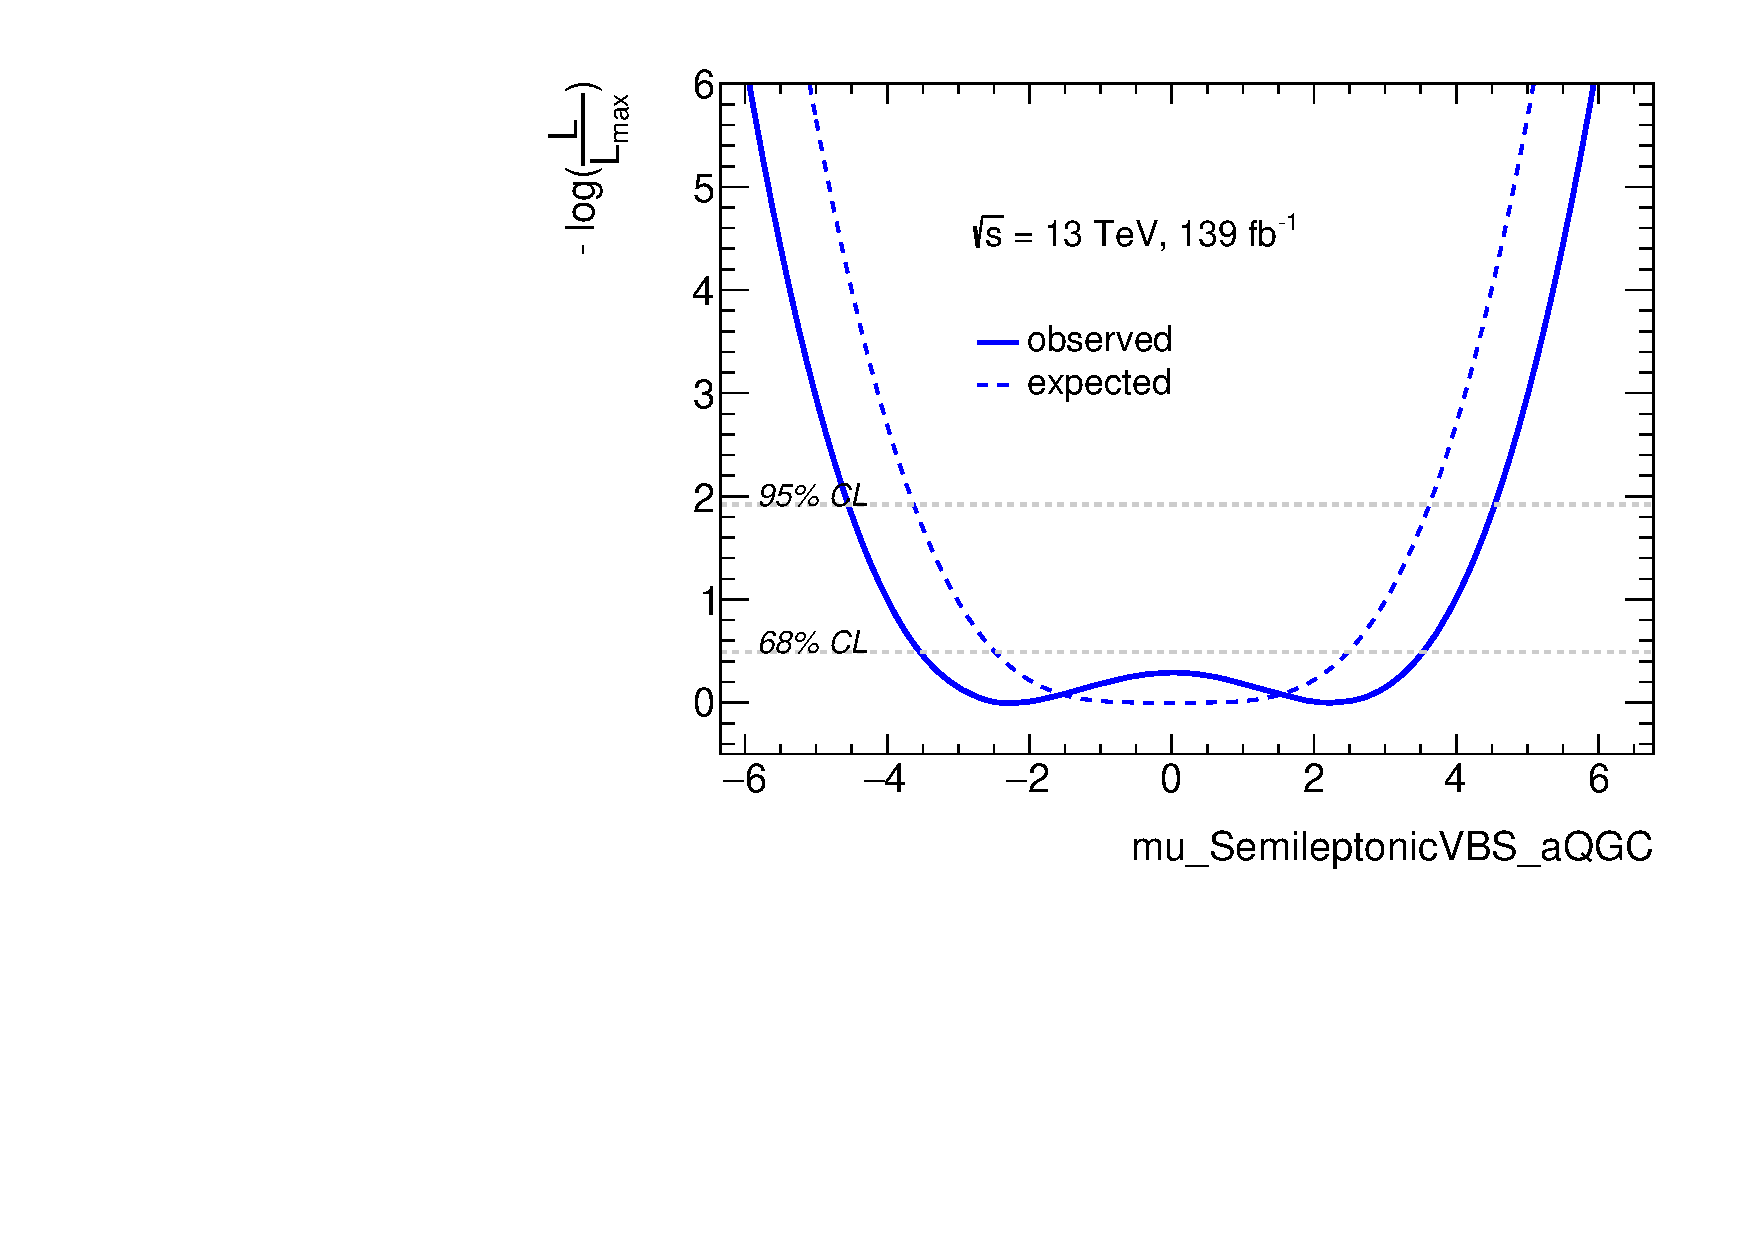
\includegraphics[width=0.32\textwidth]{figures/aQGC/profileFM22000}
    	%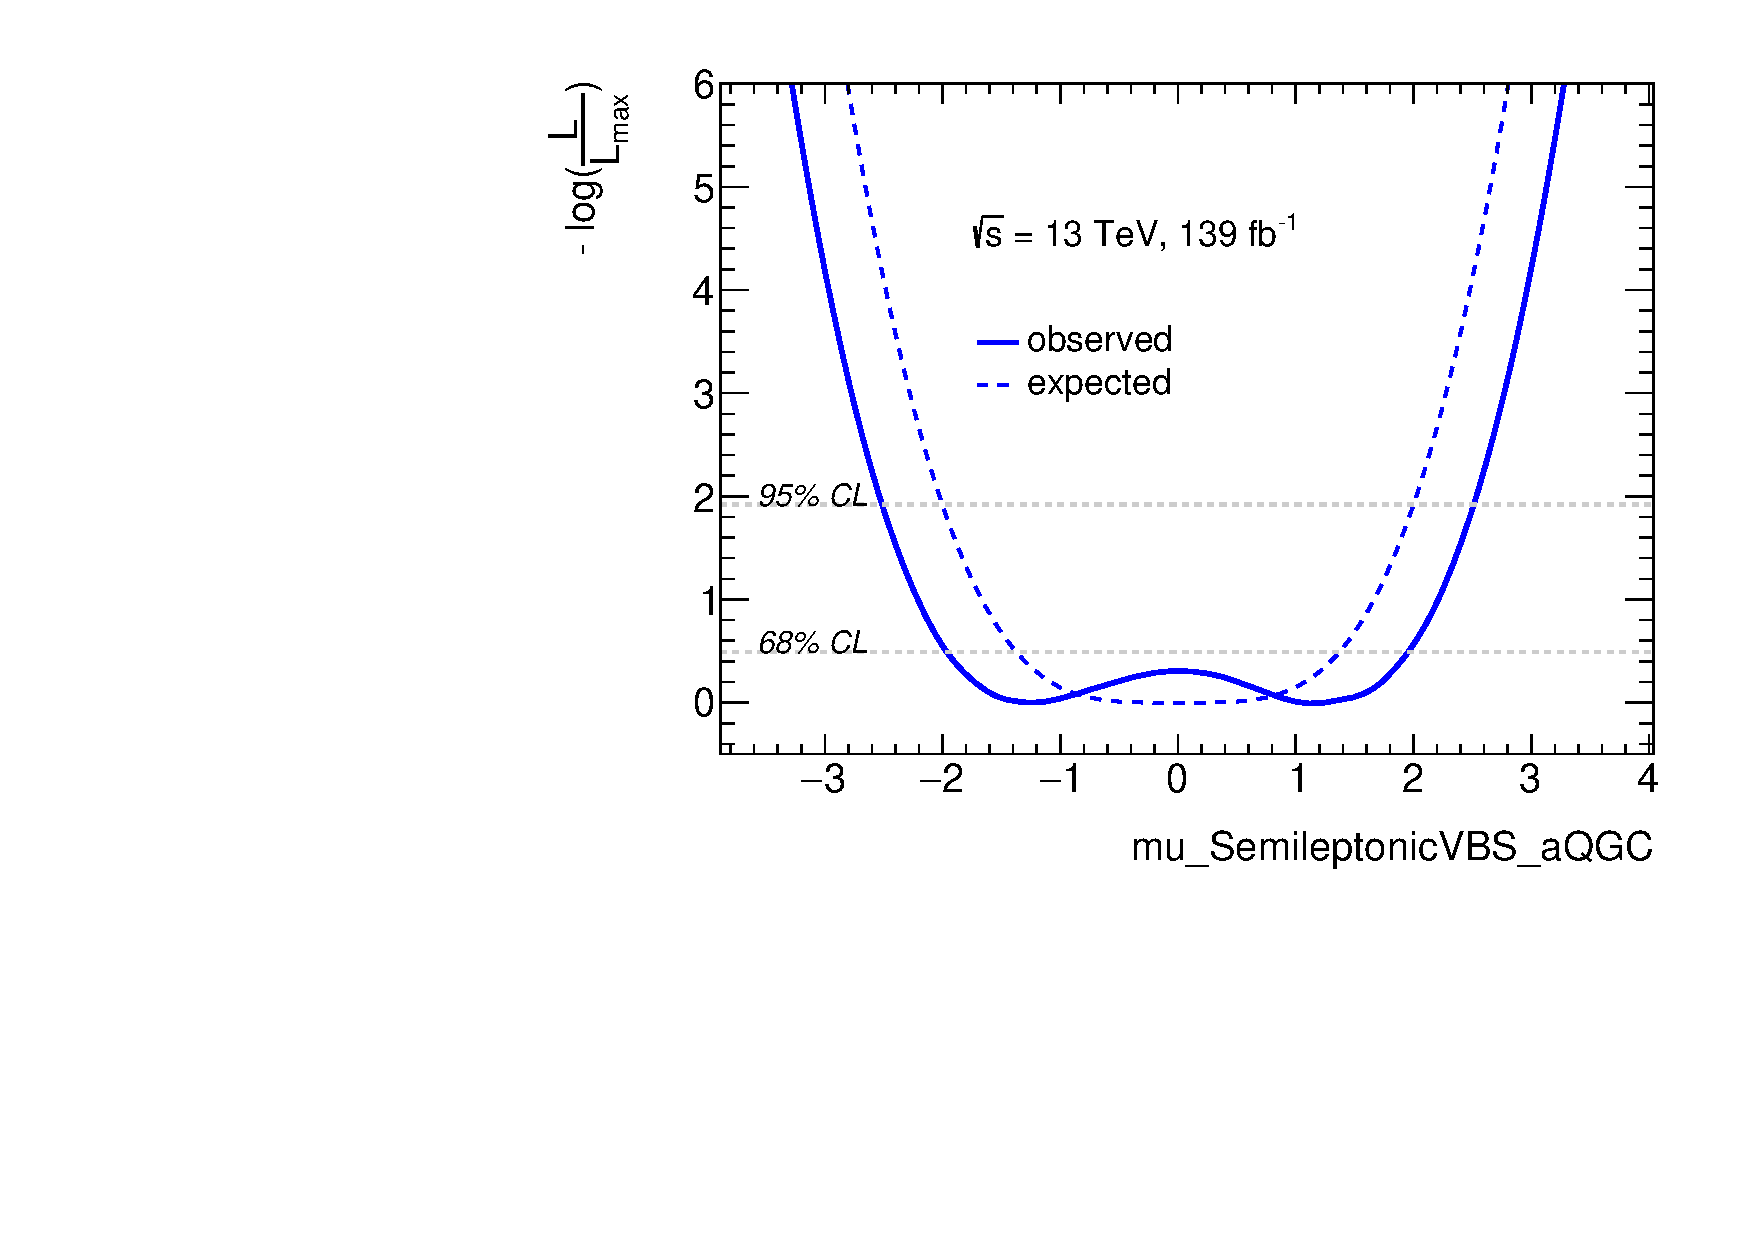
\includegraphics[width=0.38\textwidth]{figures/aQGC/profileFM23000}
        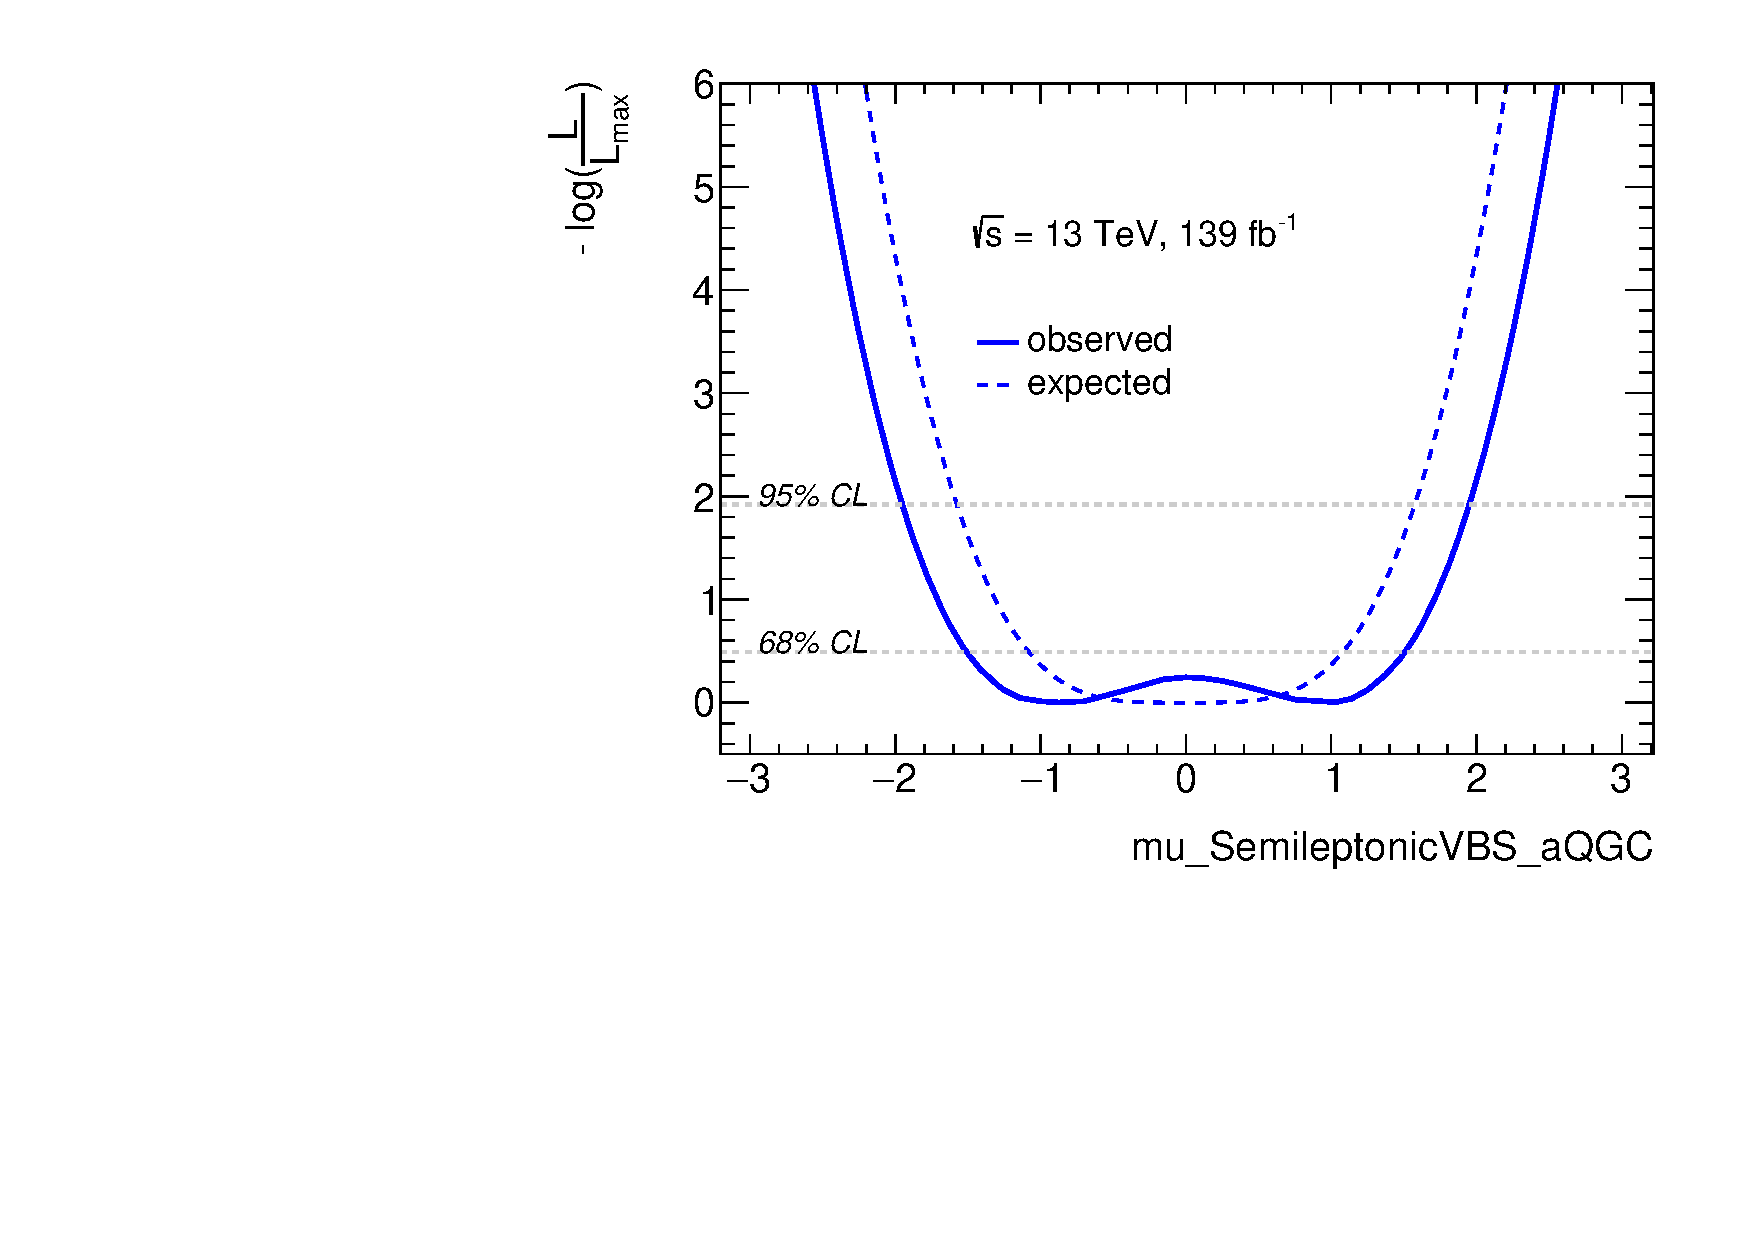
\includegraphics[width=0.32\textwidth]{figures/aQGC/profileFM2inf}
        \caption{The observed log-likelihood curves of FM2 Wilson coefficient where the clipping energy is 1.5~TeV (left), 2.0~TeV (middle), $\infty$ (right).}
        \label{fig:ProfileLL}
\end{figure}
\begin{figure}[ht]
    \centering
    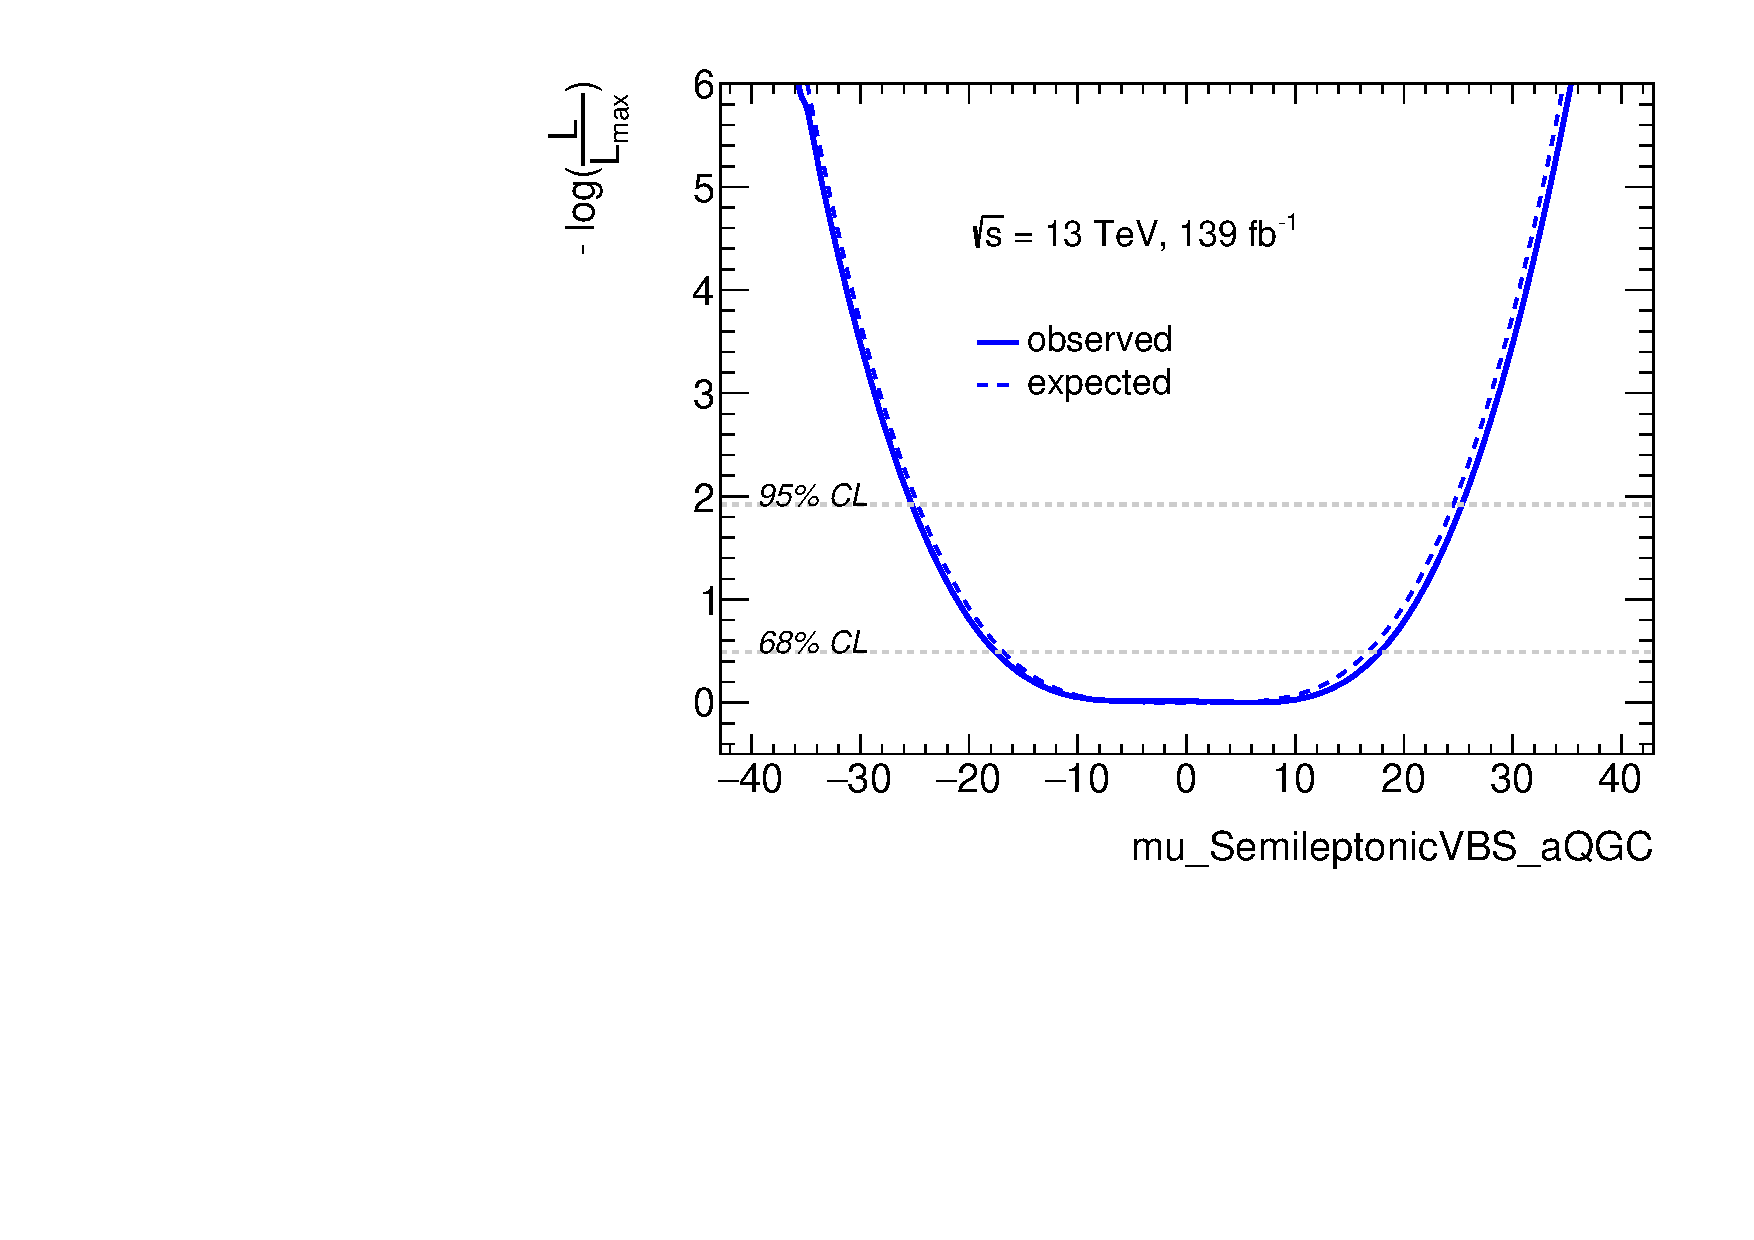
\includegraphics[width=0.32\textwidth]{figures/aQGC/profileFM31500}
    	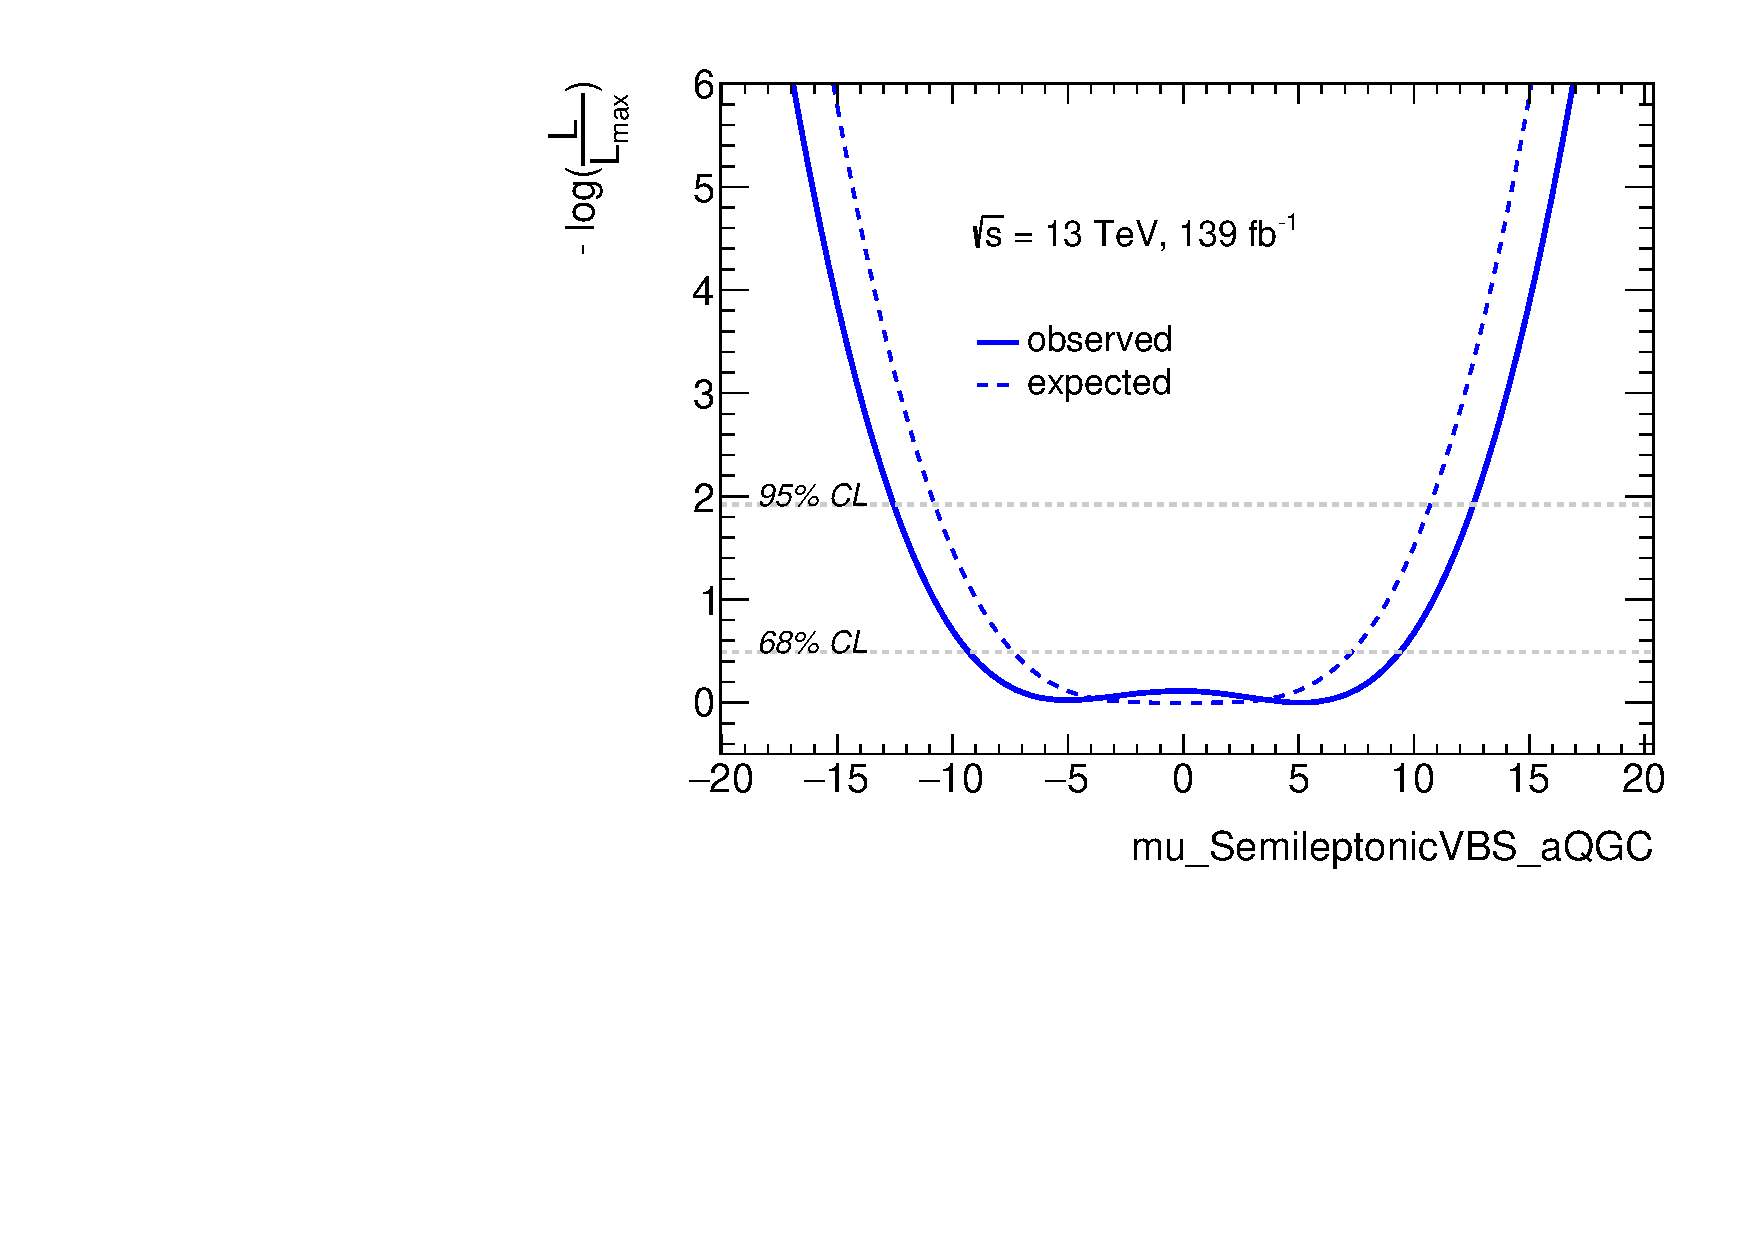
\includegraphics[width=0.32\textwidth]{figures/aQGC/profileFM32000}
    	%\includegraphics[width=0.38\textwidth]{figures/aQGC/profileFM33000}
        \includegraphics[width=0.32\textwidth]{figures/aQGC/profileFM3inf}
        \caption{The observed log-likelihood curves of FM3 Wilson coefficient where the clipping energy is 1.5~TeV (left), 2.0~TeV (middle), $\infty$ (right).}
        \label{fig:ProfileLL}
\end{figure}
\begin{figure}[ht]
    \centering
    \includegraphics[width=0.32\textwidth]{figures/aQGC/profileFM41500}
    	\includegraphics[width=0.32\textwidth]{figures/aQGC/profileFM42000}
    	%\includegraphics[width=0.38\textwidth]{figures/aQGC/profileFM43000}
        \includegraphics[width=0.32\textwidth]{figures/aQGC/profileFM4inf}
        \caption{The observed log-likelihood curves of FM4 Wilson coefficient where the clipping energy is 1.5~TeV (left), 2.0~TeV (middle), $\infty$ (right).}
        \label{fig:ProfileLL}
\end{figure}
\begin{figure}[ht]
    \centering
    \includegraphics[width=0.32\textwidth]{figures/aQGC/profileFM51500}
    	\includegraphics[width=0.32\textwidth]{figures/aQGC/profileFM52000}
    	%\includegraphics[width=0.38\textwidth]{figures/aQGC/profileFM53000}
        \includegraphics[width=0.32\textwidth]{figures/aQGC/profileFM5inf}
        \caption{The observed log-likelihood curves of FM5 Wilson coefficient where the clipping energy is 1.5~TeV (left), 2.0~TeV (middle), $\infty$ (right).}
        \label{fig:ProfileLL}
\end{figure}
\begin{figure}[ht]
    \centering
    \includegraphics[width=0.32\textwidth]{figures/aQGC/profileFM71500}
    	\includegraphics[width=0.32\textwidth]{figures/aQGC/profileFM72000}
    	%\includegraphics[width=0.38\textwidth]{figures/aQGC/profileFM73000}
        \includegraphics[width=0.32\textwidth]{figures/aQGC/profileFM7inf}
        \caption{The observed log-likelihood curves of FM7 Wilson coefficient where the clipping energy is 1.5~TeV (left), 2.0~TeV (middle), $\infty$ (right).}
        \label{fig:ProfileLL}
\end{figure}


All expected and observed limits are shown.

\begin{figure}[ht]
   \centering
   \includegraphics[width=0.45\textwidth]{figures/aQGC/ClippedFT0CI.pdf}
   \includegraphics[width=0.45\textwidth]{figures/aQGC/ClippedFT1CI.pdf}
   \includegraphics[width=0.45\textwidth]{figures/aQGC/ClippedFT2CI.pdf}
   \includegraphics[width=0.45\textwidth]{figures/aQGC/ClippedFT3CI.pdf}
   \includegraphics[width=0.45\textwidth]{figures/aQGC/ClippedFT5CI.pdf}
   \includegraphics[width=0.45\textwidth]{figures/aQGC/ClippedFT6CI.pdf}
   \includegraphics[width=0.45\textwidth]{figures/aQGC/ClippedFT7CI.pdf}
   \includegraphics[width=0.45\textwidth]{figures/aQGC/ClippedFT8CI.pdf}
   \caption{Expected limits (green) and observed limits (blue) for 5 clipping points are shown for each Wilson coefficient of FT-type. 
   The black line is the theoretical unitarity bound.}
        \label{fig:aQGClimitsFTs}
\end{figure}
\begin{figure}[ht]
   \centering
   \includegraphics[width=0.45\textwidth]{figures/aQGC/ClippedFS02CI.pdf}
   \includegraphics[width=0.45\textwidth]{figures/aQGC/ClippedFS1CI.pdf}
   \caption{Expected limits (green) and observed limits (blue) for 5 clipping points are shown for each Wilson coefficient of FS-type. 
   The black line is the theoretical unitarity bound.}
        \label{fig:aQGClimitsFSs}
\end{figure}
\begin{figure}[ht]
   \centering
   \includegraphics[width=0.45\textwidth]{figures/aQGC/ClippedFM0CI.pdf}
   \includegraphics[width=0.45\textwidth]{figures/aQGC/ClippedFM1CI.pdf}
   \includegraphics[width=0.45\textwidth]{figures/aQGC/ClippedFM2CI.pdf}
   \includegraphics[width=0.45\textwidth]{figures/aQGC/ClippedFM3CI.pdf}
   \includegraphics[width=0.45\textwidth]{figures/aQGC/ClippedFM4CI.pdf}
   \includegraphics[width=0.45\textwidth]{figures/aQGC/ClippedFM5CI.pdf}
   \includegraphics[width=0.45\textwidth]{figures/aQGC/ClippedFM7CI.pdf}
   \caption{Expected limits (green) and observed limits (blue) for 5 clipping points are shown for each Wilson coefficient of FT-type. 
   The black line is the theoretical unitarity bound.}
        \label{fig:aQGClimitsFMs}
\end{figure}
